\documentclass[a4paper,10pt]{scrbook}

% Seitenlayout
\usepackage[a4paper,top=1.5cm,right=2.0cm,bottom=2cm,left=2.0cm]{geometry}
\usepackage{lscape}
\usepackage{fancyhdr}

% Zeichen
\usepackage[ngerman]{babel}
\usepackage[utf8]{inputenc}
\usepackage{amsmath, amsthm, amssymb}
\usepackage{xcolor}
\usepackage{cancel}

% Zeichensatz
\usepackage[colorlinks,%
	    citecolor=black,%
	    filecolor=black,%
	    linkcolor=black,%
	    urlcolor=black,%
	    pdftitle = {Mitschrift - CG},%
	    pdfauthor = {Martin Lenders}%
	]{hyperref}
\usepackage{multicol}
\usepackage{listings}
\usepackage{empheq}
\usepackage{enumerate}
\usepackage{nicefrac}

% Grafik
\usepackage{graphicx}
\usepackage[usenames]{pstricks}
\usepackage{pst-node}
\usepackage{pst-plot}
\usepackage{pst-3d}
\usepackage{pst-3dplot}
\usepackage{pst-tree}
\usepackage{pst-func}
\usepackage{pst-text}
\usepackage{pstricks-add}

% Color definitions
\definecolor{lgray}{gray}{0.95}
\definecolor{save}{rgb}{0.498,0,0}
\definecolor{identifier}{rgb}{0,0,0.1}
\definecolor{string}{rgb}{0.192,0,1}
\definecolor{comment}{rgb}{0.25,0.5,0.37}
\definecolor{yellow}{rgb}{1,1,0}
\definecolor{sand}{rgb}{1,1,.75}
\definecolor{red}{rgb}{1,0,0}
\definecolor{melon}{rgb}{1,0.6,.5}
\definecolor{green}{rgb}{0,1,0}
\definecolor{lime}{rgb}{.75,1,.75}
\definecolor{blue}{rgb}{0,0,1}
\definecolor{azure}{rgb}{.75,.75,1}

\makeatletter
\pst@addfams{pst-HSB}
\define@key[psset]{pst-HSB}{HueBegin}{% Between 0 and 1
  \def\PstParametricplotHSB@HueBegin{#1}}
\define@key[psset]{pst-HSB}{HueEnd}{% Between 0 and 1
  \def\PstParametricplotHSB@HueEnd{#1}}
\define@boolkey[psset]{pst-HSB}[Pst@]{HSB}[true]{}
% Default values
\psset[pst-HSB]{HueBegin=0,HueEnd=1,HSB=true}
\psset{dimen=outer}

% Einstellungen für Pakete
\lstset{
	tabsize=8,
	frame=,
	basicstyle=\footnotesize\changefont{pcr}{m}{n},
	emphstyle=\textit,
	language=Java,
	numberstyle=\tiny\textsf,
	numbersep=5pt,
	numbers=none,
	keywordstyle=\color{save}\textbf,
	identifierstyle=\color{identifier},
	stringstyle=\color{string},
	backgroundcolor=\color{lgray},
	showstringspaces=false,
	commentstyle=\color{comment},
	extendedchars=true,
	xleftmargin=1em,
	inputencoding=utf8,
	mathescape=true;
}

\psset{%
	algebraic=true,
	angleA=0,%
	angleB=180,%
	unit=1cm,%
	subgriddiv=0,%
	griddots=5,%
	gridlabels=7pt%
}

\renewcommand{\chaptermark}[1]{markboth{#1}{}}
\renewcommand{\sectionmark}[1]{\markright{\thesection\ #1}}
\pagestyle{fancy}
\fancyhf{}
\fancyfoot[LE,RO]{\sffamily\thepage}
\fancyhead[LE]{\footnotesize\sffamily\bfseries\leftmark}
\fancyhead[RO]{\footnotesize\sffamily\rightmark} 

% Eigene Befehle
\newcommand{\changefont}[3]{\fontfamily{#1} \fontseries{#2} \fontshape{#3} \selectfont}
\newcommand{\Defi}{\paragraph*{Definition}}
\newcommand{\Lemma}{\paragraph*{Lemma}}
\newcommand{\Satz}{\paragraph*{Satz}}
\newcommand{\Bew}{\paragraph*{Beweis}}
\newcommand{\Bsp}{\paragraph*{Beispiel}}
\newcommand{\rg}{\operatorname{rg}}
\newcommand{\vtwo}[2]{\begin{pmatrix}#1\\#2\end{pmatrix}}
\newcommand{\vthree}[3]{\begin{pmatrix}#1\\#2\\#3\end{pmatrix}}
\newcommand{\xyz}{\vthree{x}{y}{z}}
\newcommand{\vfour}[4]{\begin{pmatrix}#1\\#2\\#3\\#4\end{pmatrix}}

% Neudefinitionen
\renewcommand{\texttt}{\changefont{pcr}{m}{n}}
\renewcommand{\thepart}{\Alph{part}}
\renewcommand{\sectionmark}[1]{\markright{\thesection\ #1}}

\title{Mitschrift\\{\LARGE Computergrafik}}
\author{gehalten von Prof. Dr. Günther Rote}
\subject{Achtung: Dieses Dokument ist \emph{nur} eine Mitschrift der Vorlesung "Computergrafik" SoSe2010.
	Sie wurde während der Vorlesung angefertigt. Es wird aber seitens des Autors keine Garantie auf
	Vollständigkeit und Richtigkeit des Inhalts gegeben.}

\begin{document}
\maketitle
\tableofcontents
\chapter{Einführung}
\section{Organisatorisches}
\subsection{Übungsblätter:}
\begin{itemize}
 \item Ausgabe: Mittwoch, Abgabe: Freitag
 \item Abgabe in Zweiergruppen
 \item 60\% der Punkte müssen erreicht werden
 \item min. einmal Vorrechnen
\end{itemize}

\subsection{Programmierung}
\begin{itemize}
 \item Aufgaben in Java gestaltet
 \item mit OpenGL-Interface
 \item auf Nachfrage kann auch C/C++ verwendet werden
\end{itemize}

\section{Übersicht}
\begin{center}
\begin{psmatrix}
 \rnode{GM}{
 \begin{minipage}{3cm}
  \centering
  Geometrisches Modell\\(im Computer)
 \end{minipage}
 } & \rnode{B1}{Bild} & \\
 \rnode{PH}{Punkthaufen} && \rnode{A}{Auge} & \rnode{G}{Gehirn}\\
 \rnode{W}{Wirklichkeit} & \rnode{B2}{Bild}
 \ncline{GM}{B1}
 \ncline{PH}{GM}
 \ncline{W}{PH}\naput[nrot=90]{\textit{\footnotesize Laserscanner}}
 \ncline{W}{B2}\nbput{\textit{\footnotesize Kamera}}
 \ncline{B2}{GM}
 \ncline{B2}{A}
 \ncline{B1}{A}
 \ncline{W}{A}
 \ncline{A}{G}
 \ncbox[linearc=0.3,boxsize=1cm,nodesep=5pt,linecolor=red]{1,1}{1,2}
 \ncbox[linearc=1.5,boxsize=1.5cm,nodesep=10pt,linecolor=green]{1,1}{3,2}
 \ncbox[linearc=0.3,boxsize=1.5cm,nodesep=5pt,linecolor=blue]{1,1}{2,1}
\end{psmatrix}
\end{center}

\begin{itemize}
 \item \textsc{\color{red}Computergrafik}
 \item \textsc{\color{green}Bildbearbeitung / Bilderkennung}
 \item \textsc{\color{blue}Geometrisches Rechnen / Geometrische Modellierung}
\end{itemize}

\subsection{Fahrplan}
\begin{itemize}
 \item Koordinatiensysteme, geometrische Transformationen
 \item Licht und Farben
 \item Rasterung
 \item Beleuchtung und Schattierung
 \item rendering-pipeline: vom Modell bis zum gerasterten Bildbearbeitung
 \item geometrische Modellierung: Kurven, Flächen und Splines
 \item {\color{red}\large Kein Anwendungskurs für OpenGL, JOGL, Javaview etc.!}
\end{itemize}


\chapter{Koordinatensysteme, geometrische Transformationen}
\section{kartesische Koordinaten}
\begin{center}
\begin{pspicture}[unit=0.5cm](0,0)(5,3)
	\psaxes[Dx=2,Dy=2](0,0)(0,0)(10,6)[$x$,0][$y$,0]
	\psdot(5,3)\rput[bl](5,3){$p = \vtwo{x}{y} = \vtwo{5}{3}$}
\end{pspicture}
\end{center}

\section{Geometrische Transformationen}
\begin{itemize}
 \item \emph{Tranlation}: $p \mapsto p + t \qquad t \in \mathbb{R}^2$,  Translationsvektor
	\begin{center}
	 \begin{pspicture}[unit=0.5cm](0,0)(4,4)
	  \psaxes[labels=none,ticks=none](0,0)(0,0)(8,8)
	  \pspolygon[linestyle=dotted](6,5)(7,7.5)(2,8)(3,3)
	  \rput[lb](5,3){\psline[linecolor=red](0,0)(1,2)\uput{3pt}[r]{0}(0.5,1){\color{red}$t$}}
	  \rput[lb](6,5.5){\psline[linecolor=red](0,0)(1,2)\uput{3pt}[r]{0}(0.5,1){\color{red}$t$}}
	  \rput[lb](1,6){\psline[linecolor=red](0,0)(1,2)\uput{3pt}[r]{0}(0.5,1){\color{red}$t$}}
	  \rput[lb](2,1){\psline[linecolor=red](0,0)(1,2)\uput{3pt}[r]{0}(0.5,1){\color{red}$t$}}
	  \pspolygon(5,3)(6,5.5)(1,6)(2,1)
	  \psdot(5,3)
	  \psdot(6,5.5)
	  \psdot(1,6)
	  \psdot(2,1)
	 \end{pspicture}
	\end{center}

 \item \emph{Rotation} (um den Ursprung $\vtwo{0}{0}$):
	\[p \mapsto M \cdot p \qquad M = \begin{pmatrix}
	                                  \cos{\alpha} & -\sin{\alpha} \\
	                                  \sin{\alpha} & \cos{\alpha}
	                                 \end{pmatrix}\text{, Rotationsmatrix}\]
	\begin{center}
	 \begin{pspicture}[unit=0.5cm](-2,-2)(2,2)
	  \psaxes[labels=none,ticks=none](0,0)(-4,-4)(4,4)
	  \SpecialCoor
	  \rput[tl](-4,4){\color{red}$\alpha = 20^\circ$}
	  \psarc[linecolor=red](0,0){3}{30}{50}\uput{3pt}[40]{0}(3;40){\color{red}$\alpha$}
	  \psarc[linecolor=red](0,0){4}{135}{155}\uput{3pt}[145]{0}(4;145){\color{red}$\alpha$}
	  \psarc[linecolor=red](0,0){2}{-70}{-50}\uput{3pt}[-60]{0}(2;-60){\color{red}$\alpha$}
	  \pspolygon(3;30)(4;135)(2;-70)
	  \pspolygon[linestyle=dotted](3;50)(4;155)(2;-50)
	 \end{pspicture}
	\end{center}
 \item \emph{Rotation} um den Punkt $c$: $p \mapsto M(p -c) + c = Mp + (c - Mc), \qquad c \mapsto c$
 \item \emph{gleichförmige Skalierung}:
	\begin{align*}
	&&p &\mapsto \lambda \cdot p = \begin{pmatrix}
	                               \lambda & 0 \\
	                               0 & \lambda
	                              \end{pmatrix} \cdot p, \qquad \lambda \neq 0\\
	&\lambda = 1& p &\mapsto -p = \begin{pmatrix}
	                                     -1 & 0 \\
	                                     0 & -1
	                                    \end{pmatrix} \cdot p = \text{Spiegelung am Ursprung $=$ Rotation um $180^\circ$}
	\end{align*}
 \item \emph{Ungleichförmige Skalierung}:
	\[M = \begin{pmatrix}
	       \lambda_1 & 0 \\
	       0 & \lambda_2
	      \end{pmatrix} \qquad p \mapsto M \cdot p\]
	\[\vtwo{x}{y} = \vtwo{\lambda_1 x}{\lambda_2 y}\]
	\[M = \begin{pmatrix}
	       -1 & 0 \\
	       0 & 1
	      \end{pmatrix} \text{resultiert in der Spiegelung an der $x$-Achse}\]
	\[M = \begin{pmatrix}
	       1 & 0 \\
	       0 & -1
	      \end{pmatrix} \text{resultiert in der Spiegelung an der $y$-Achse}\]
 \item \emph{Scherung}
	\[M = \overset{\text{Scherung auf der $x$-Achse}}{\begin{pmatrix}
		1 &  \lambda \\
		0 & 1
	      \end{pmatrix}} \left(\text{oder } \overset{\text{Scherung auf der $y$-Achse}}{\begin{pmatrix}
		1 & 0 \\
		\lambda & 1 \\
	      \end{pmatrix}}
	      \right)\]
	      \[\vtwo{x}{y} \mapsto \begin{pmatrix}
		1 &  \lambda \\
		0 & 1
	      \end{pmatrix} \vtwo{x}{y} = \vtwo{x+ \lambda y}{y}\]
	 \begin{center}
	 \begin{pspicture}[unit=0.5cm](0,0)(4,2.1)
	  \rput[tl](0.1,4){\color{red}$\lambda = 0{,}5$}
	  \psaxes[labels=none,ticks=none](0,0)(0,0)(8,4.2)
	  \psline[linecolor=red](4,1)(4.5,1)
	  \psline[linecolor=red](4,2)(5,2)
	  \psline[linecolor=red](4,3)(5.5,3)
	  \psline[linecolor=red](4,4)(6,4)
	  \psdot(4,1)\psdot[dotstyle=o](4.5,1)
	  \psdot(4,2)\psdot[dotstyle=o](5,2)
	  \psdot(4,3)\psdot[dotstyle=o](5.5,3)
	  \psdot(4,4)\psdot[dotstyle=o](6,4)
	 \end{pspicture}
	\end{center}
\end{itemize}
Flächeninhalt:
\begin{itemize}
 \item Translationen, Rotationen, Scherungen und Spiegelungen ändern den Flächeninhalt \underline{nicht}.
 \item Skalierung ändert den Flächeninhalt um den Faktor $\lambda_1 \cdot \lambda_2$
\end{itemize}

\Defi Eine Verknüpfung mehrerer dieser Transformationen bildet eine \textbf{affine Transformation}.
	Allgemein ist diese:
	\[ p \mapsto M \cdot p = b, \qquad M \in \mathbb{R}^{2 \times 2}, b \in \mathbb{R}^2, \det M \neq 0 \]
	Der Flächeninhalt ändert sich um den Faktor $\det M$

\Defi Die Verknüpfung von Translation, Rotation und Spiegelung heißt \textbf{starre Bewegung} oder \textbf{Isometrie}.
	Allgemein ist diese:
	\[ p \mapsto Mp + t \text{ mit \textbf{orthogonaler Matrix} $M$ (d. h. $\det M = \pm 1$)}\]
	die Isometrien zerfallen:
	\begin{itemize}
	 \item \textbf{orientierungserhaltende} ($\det M = 1$) und
	 \item \textbf{orientierungsumkehrende} ($\det M = -1$) Isometrien
	\end{itemize}

\section{Homogene Koordinaten}
\Defi \textbf{Homogene Koordinaten}: Statt $p = \vtwo{x}{y}$ verwendet man eine dritte Koordinate
	$p = \vthree{x}{y}{1}$

\paragraph*{Konvention} Die Koordinaten $\vthree{x}{y}{z}$ und
	$\vthree{\lambda x}{\lambda y}{\lambda z}$ stellen denselben Punkt dar ($\lambda \neq 0$)

Der Punkt $\vthree{x}{y}{z}$ mit $z \neq 0$ hat die kartesischen Koordinaten $\vtwo{\frac{x}{z}}{\frac{y}{z}}$

\subsection{Allgemeine affine Transformation in homogenen Koordinaten}
\[\vthree{x}{y}{z} \mapsto \underbrace{\begin{pmatrix}
				m_{11} & m_{12} & b_1\\
				m_{21} & m_{22} & b_2\\
				0 & 0 & 1
                           \end{pmatrix}}_{M'} \cdot \vthree{x}{y}{z}\]
\[\vthree{x}{y}{1} \mapsto \vthree{m_{11}x + m_{12}y + b_1}{m_{21}x + m_{22}y + b_2}{1}\]

Die Matrizen $M'$ und $\lambda M'$ beschreiben dieselbe Transformation $(\lambda \neq 0)$

\[p \mapsto M' p \text{ mit } M' = \begin{pmatrix}
                                    m_{11} & m_{12} & m_{13} \\
                                    m_{21} & m_{22} & m_{23} \\
                                    0 & 0 & m_{33}
                                   \end{pmatrix} \text{ und $\det M' \neq 0$}
\]
\[\det M' \neq 0 \Leftrightarrow m_{33} \neq 0 \land \begin{vmatrix}
                                                    m_{11} & m_{12} \\
                                                    m_{21} & m_{22}
                                                   \end{vmatrix} \neq 0
\]
$\Rightarrow$ o. B. d. A. kann man auch $m_{33} = 1$ annehmen (Dann kann man die dritte Zeile auch weglassen).

\section{Die projektive Ebene}
\Defi Die (reelle) \textbf{projektive Ebene} $P^2$ besteht aus den Äquivalenzklassen von Punkten
	$\vthree{x}{y}{z} \neq \vthree{0}{0}{0}$, wobei $\vthree{x}{y}{z}$ und $\vthree{\lambda x}{\lambda y}{\lambda z}$
	denselben Punkt darstellen ($\lambda \neq 0$)

\subsection{Geraden in der projektiven Ebene}
Gerade in $\mathbb{R}^2$ (karthesische Koordinaten):
 \[y = ax + b \text{(Gerade darf nicht senkrecht sein)}\]
 \[ax + by = -c\]

\[\Updownarrow\]
Gerade in Homogenen Koordinaten
\[\vtwo{x}{y} \longrightarrow \vthree{x}{y}{1}\]
\[ax + by + c = 0 \Leftrightarrow \vthree{a}{b}{c} \cdot \vthree{x}{y}{1} = 0\]
Allgemeine Gleichung einer Geraden in $P^2$
\[\vthree{a}{b}{c} \cdot \vthree{x}{y}{z} = 0 \Leftrightarrow ax + by + cz = 0 \qquad \vthree{a}{b}{c} \neq \vthree{0}{0}{0}\]
Wenn $\vthree{x}{y}{z}$ die Gleichung erfüllt, dann erfüllt auch $\vthree{\lambda x}{\lambda y}{\lambda z}$ die Gleichung.
$\vthree{a}{b}{c}$ und $\vthree{\lambda a}{\lambda b}{\lambda c}$ stellen dieselbe Gerade dar.

\begin{description}
 \item[projektive Punkte] $\vthree{x}{y}{z} \neq \vthree{0}{0}{0}$ Skalierung egal.
 \item[projektive Gerade] $\vthree{a}{b}{c} \neq \vthree{0}{0}{0}$ Skalierung egal
\end{description}
\Satz Punkt $\vthree{x}{y}{z}$ liegt auf der Geraden $\vthree{a}{b}{c}$:
\[\vthree{a}{b}{c} \cdot \vthree{x}{y}{z} = 0\]

\Satz	Zwei verschiedene Geraden schneiden sich in genau einem Punkt.
\Bew	Gerade $\forall \lambda: \vthree{a_1}{b_1}{c_1}, \vthree{a_2}{b_2}{c_2} \neq \lambda \vthree{a_1}{b_1}{c_1}$.
Schnittpunkt:
\begin{align*}
 a_1 x + b_1 y + c_1 z &= 0\\
 a_2 x + b_2 y + c_2 z &= 0
\end{align*}
Koeffizientenmatrix $A = \begin{pmatrix}
                          a_1 & b_1 & c_1 \\
                          a_2 & b_2 & c_2
                         \end{pmatrix}, \rg A = 2$\\
$\Rightarrow$ Lösungsmenge ist eindimensional
\[ L = \left\{\left.\lambda \vthree{x_0}{y_0}{z_0} \right| \lambda \in \mathbb{R}\right\} \text{ist ein projektiver Punkt}\]
$\vthree{x_0}{y_0}{z_0}$ kann als $\vthree{a_1}{b_1}{c_1} \times \vthree{a_2}{b_2}{c_2} = \vthree{
		\begin{vmatrix}
		 b_1 & b_2 \\
		 c_1 & c_2
		\end{vmatrix}\\}{
		\begin{vmatrix}
		 c_1 & c_2 \\
		 a_1 & a_2
		\end{vmatrix}\\}{
		\begin{vmatrix}
		 a_1 & a_2 \\
		 b_1 & b_2
		\end{vmatrix}}
$ berechnet werden (Kreuzprodukt)

\begin{center}
	\psset{Alpha=150,Beta=20,unit=1.5cm,arrows=->}
	\begin{pspicture}(-1,0)(3,2.8)
		\rput[bl]{15}(0,0){
		\pstThreeDSquare[fillstyle=hlines,hatchcolor=gray,linecolor=gray,arrows=-](0,0,0)(1.3,0,0)(0,1.8,0)
		\pstThreeDSquare[arrows=-](0,0,0)(0.5,0,0)(0,0,0.5)
		\pstThreeDDot(0.25,0,0.25)
		\pstThreeDSquare[arrows=-](0,0,0)(0,0.5,0)(0,0,0.5)
		\pstThreeDDot(0,0.25,0.25)
		\pstThreeDLine(0,0,0)(1.5,0,0)\pstThreeDPut(1.6,0,0){$\vec u$}
		\pstThreeDLine(0,0,0)(0,2,0)\pstThreeDPut(0,2.1,0){$\vec v$}
		\pstThreeDLine(0,0,3)\pstThreeDPut(0,0,3.1){$\vec u \times \vec v$}
		}
	\end{pspicture}
\end{center}


\Satz Durch zwei verschiedene Punkte gibt es genau eine Geraden

\Bew gleich wie oben: $\vthree{a}{b}{c}$ mit $\vthree{x}{y}{z}$ vertauschen.

\paragraph*{Dualitätsprinzip} Man kann in einem Satz der projektiven Geometrie der Ebene "`Punkte"' und "`Geraden"'
	vertauschen und es bleibt ein gültiger Satz.
	
\pagebreak
\subsection{Modelle der projektiven Ebene}
\begin{enumerate}
 \item \emph{Räumliches Modell der projektiven Ebene}
	$\left\{\left.\lambda \vthree{x_0}{y_0}{z_0}\right| \lambda \in \mathbb{R}\right\}$...
		Geraden durch den Ursprung im $\mathbb{R}^3$ entsprechen den projektiven Punkten.
	\begin{center}
	 \begin{pspicture}(-5,-2)(5,4)
	  \pstThreeDCoor[xMin=-4,xMax=4,yMin=-4,yMax=4]
	  \pstThreeDLine{-}(-4,2,0)(4,-2,0)
	  \pstThreeDLine{-}(-2,-4,0)(2,4,0)
	  \pstThreeDLine{-}(3,-1.5,0)(-1.5,-3,0)(-3,1.5,0)(1.5,3,0)(3,-1.5,0)
	 \end{pspicture}
	\end{center}
	\begin{center}
	 projektive Gerade $\equiv$ Ebene durch den Ursprung
	\end{center}

\item \emph{Kugelmodell der projektiven Ebene}
	entsteht durch Schnitt des räumlichen Modells mit der Einheitskugel $S^2 =
		\left\{\left.\vthree{x}{y}{z}\right| x^2 + y^2 + z^2 = 1\right\}$
	
	\begin{center}
	 \begin{pspicture}(-5,-3)(5,3)
	  \psset{arrows=-}
	  \psellipticarc[linestyle=dashed]{-}(0,0)(2,1){0}{180}
	  \pstThreeDCoor[xMin=-4,yMin=-4,zMin=-3]
	  \pstThreeDLine{-}(-4,2,0)(4,-2,0)
	  \pstThreeDLine{-}(-2,-4,0)(2,4,0)
	  
	  \pstThreeDLine{-}(4,2,0)(-4,-2,0)
	  \pstThreeDDot(1.8,0.9,0)
	  \pstThreeDDot(-1.8,-0.9,0)

	  \pstThreeDCircle[Alpha=55,Beta=10](1.153,1.153,-1.153)(-.2,.2,0)(.231,.231,.231)
	  
	  \pscircle(0,0){2}
	  \psellipticarc{-}(0,0)(2,1){180}{0}

	  \pstThreeDNode(0,-2,0){GK}
	  \rput[tl](-3,2){\rnode{GK_label}{Großkreis}}
	  \ncline{->}{GK_label}{GK}
	  \pnode(1.4,1.4){EK}
	  \rput[tl](3,3){\rnode{EK_label}{Einheitskugel}}
	  \ncline{->}{EK_label}{EK}

	  \pstThreeDNode[Alpha=55,Beta=10](1.153,1.153,-1.153){kGK}
	  \rput[tl](3,-2){\Rnode[href=-0.9]{kGK_label}{kein Großkreis}}
	  \ncline[nodesepB=5px]{->}{kGK_label}{kGK}
	 \end{pspicture}
	\end{center}
	\begin{align*}
	 \text{projektiver Punkt} &\equiv \text{Paar gegenüberliegender Punkte auf der Einheitskugel}\\
	 \text{projektive Gerade} &\equiv \text{Großkreise}
	\end{align*}
\end{enumerate}


\subsection{Projektive Punkte zu karthesische Koordinaten}
\begin{center}
	 \begin{pspicture}(-5,-2)(5,4)
	  \psset{arrows=-}
	  \psellipticarc[linestyle=dashed]{-}(0,0)(2,1){0}{180}
	  \pstThreeDCoor[xMin=-4,yMin=-4,zMin=-3]

	  \pstThreeDSquare(-2,-2,2)(6,0,0)(0,6,0)

	  \pstThreeDLine(0.2,1,-2)(-0.4,-2,4)
	  \pstThreeDLine(-3,-9,-6)(3,9,6)
	  
	  \pstThreeDDot(0,0,2)
	  \pstThreeDDot[drawCoor=true](-0.2,-1,2)
	  \pstThreeDDot[drawCoor=true](1,3,2)

	  \pstThreeDPut(-3,2,2){$\vthree{\frac{x}{z}}{\frac{y}{z}}{1}$}
	  
	  \pscircle(0,0){2}
	  \psellipticarc{-}(0,0)(2,1){180}{0}

	  \pstThreeDNode[Alpha=75](1.4,1.4,0){aq}
	  \rput[tl](3,-2){\Rnode[href=-0.9]{aq_label}{Äquator = Ferngerade}}
	  \ncline[nodesepB=5px]{->}{aq_label}{aq}
	 \end{pspicture}
\end{center}
Schnitt der Geraden $\vthree{x}{y}{z} \cdot \lambda$ im $\mathbb{R}^3$ mit Ebene $z = 1$:
$z \cdot \lambda = 1 \Rightarrow \lambda = \dfrac{1}{z}$\\
$\rightarrow \vthree{x \cdot \frac{1}{z}}{y \cdot \frac{1}{z}}{1}$

\Satz Die Punkte $\vthree{x}{y}{z}$ mit $z = 0$ haben \emph{keine} Entsprechung in der euklidischen Ebene:
Jede projektive Gerade hat als Bild in der euklidischen Ebene eine Gerade, mit einer Ausnahme: die Gerade
$\vthree{0}{0}{1}$

\Defi Die Punkte des projektiven Raumes, die keine euklidische Entsprechung haben, heißen \textbf{Fernpunkte}.
	Die Gerade $\vthree{0}{0}{1}$ \textbf{Ferngerade}.

\Satz Zwei Geraden der euklidischen Ebene sind genau dann \emph{parallel}, wenn ihr Schnittpunkt ein Fernpunkt ist.

\Satz Die Punkte, die auf der Ferngeraden liegen, sind genau die Fernpunkte

\Satz Es gibt zu jeder Schaar paralleler Geraden genau einen Fernpunkt.
\begin{center}
 \begin{pspicture}(0,0)(5,4)
	\psset{arrows=-}
	\rput[lb](0.5,1.75){\psline(0,0)(2.25,2.25)}
	\rput[lb](1,1.5){\psline(0,0)(2.25,2.25)}
	\rput[lb](1.5,1.25){\psline(0,0)(2.25,2.25)}
	\rput[lb](2,1){\psline(0,0)(2.25,2.25)}
	\rput[lb](2.5,0.75){\psline(0,0)(2.25,2.25)}
	\psbrace[nodesepB=2pt,ref=rC](0.25,1.75)(2.65,0.5){\psdot[dotsize=4pt](0,0)}
 \end{pspicture}
\end{center}

Anschaulich ist ein Fernpunkt äquivalent zu perspektivischen Sammelpunkten:
\begin{center}
 \begin{pspicture}(-3,-2)(0,0)
	\psset{arrows=-}
	\psdot(0,0)
	\rput[bl](0.1,0){Fernpunkt}
	\psline[linestyle=dotted](0,0)(-2,-2)
	\psline[linestyle=dotted](0,0)(-3,-2)
	\pspolygon(-2,-2)(-0.5,-0.5)(-0.75,-0.5)(-3,-2)
 \end{pspicture}
\end{center}

\section{Allgemeine projektive Transformationen}
$\xyz \mapsto M \cdot \xyz$ mit $M = \mathbb{R}^{3 \times 3}, \det M \neq 0$\\
(Punkte bleiben Punkte, Geraden bleiben Geraden, Inzidenz bleibt erhalten)

\Defi Affine Transformationen sind jene Transformationen, bei denen die Fernpunkte Fernpunkte bleiben.
\[ \vthree{x}{y}{z} \mapsto M \vthree{x}{y}{0} = \vthree{x'}{y'}{z'} \stackrel{!}= \vthree{x'}{y'}{0}\]
\[M = \begin{pmatrix}
       m_{11} & m_{12} & m_{13} \\
       m_{21} & m_{22} & m_{23} \\
       \cancel{m_{31}}{0} & \cancel{m_{32}}{0} & m_{33}
      \end{pmatrix}
\]
\begin{align*}
 \forall x, y: m_{31} x + m_{32} y + m_{33} \cdot 0 = 0 &\Rightarrow m_{31} = m_{32} = 0
\end{align*}

\begin{align*}
 \det M &\neq 0\\
 \det M &= \underbrace{m_{33}}_{\neq 0} \cdot \underbrace{\begin{vmatrix}m_{11}&m_{12}\\m_{21}&m_{22}\end{vmatrix}}_{0}
	&\Rightarrow \text{o. B. d. A. $m_33 = 1$}
\end{align*}

\[\vtwo{x}{y} \mapsto \overbrace{\begin{pmatrix}m_{11}&m_{12}\\m_{21}&m_{22}\end{pmatrix}
	\vtwo{x}{y}}^{\text{lineare Transformation}} + \overbrace{\vtwo{m_{13}}{m_{23}}}^{\text{+ Translation}}\]

Affine Transformation:
\begin{itemize}
 \item parallele Geraden bleiben parallel
	\begin{center}
	 \begin{pspicture}(0,-0.5)(12,3.5)
	  \psframe[fillstyle=hlines,linestyle=none](0,1)(1,2)
	  \psframe[fillstyle=hlines,linestyle=none](2,0)(3,1)
	  \psellipse[fillstyle=hlines](4,0.5)(0.5,0.5)
	  \psline{-}(0.5,1.8)(0.5,2.2)
	  \psline{-}(0,-0.2)(0,3.2)
	  \psline{-}(1,-0.2)(1,3.2)
	  \psline{-}(2,-0.2)(2,3.2)
	  \psline{-}(3,-0.2)(3,3.2)
	  \psline{-}(-0.2,0)(3.2,0)
	  \psline{-}(-0.2,1)(3.2,1)
	  \psline{-}(-0.2,2)(3.2,2)
	  \psline{-}(-0.2,3)(3.2,3)

	  \psline[linewidth=2px]{-}(1,3)(2,3)
	  \psline[linewidth=2px]{-}(0,0)(1,0)
	  
	  \psline[linewidth=3px](5,1.5)(7,1.5)

	  \pspolygon[fillstyle=hlines,linestyle=none,hatchangle=71.57](7.5,0.25)(7.5,1.25)(8.5,1.75)(8.5,0.75)
	  \pspolygon[fillstyle=hlines,linestyle=none,hatchangle=71.57](9.5,0.25)(9.5,1.25)(10.5,1.75)(10.5,0.75)
	  \rput{26.57}(11.5,1.75){\psellipse[fillstyle=hlines](0,0)(0.559,0.5)}
	  \psline{-}(8,1.3)(8,1.7)
	  \psline{-}(7.5,-0.95)(7.5,2.45)
	  \psline{-}(8.5,-0.45)(8.5,2.95)
	  \psline{-}(9.5,0.05)(9.5,3.45)
	  \psline{-}(10.5,0.55)(10.5,3.95)
	  \psline{-}(7.3,-0.85)(10.7,0.85)
	  \psline{-}(7.3,0.15)(10.7,1.85)
	  \psline{-}(7.3,1.15)(10.7,2.85)
	  \psline{-}(7.3,2.15)(10.7,3.85)

	  \psline[linewidth=2px]{-}(8.5,2.75)(9.5,3.25)
	  \psline[linewidth=2px]{-}(7.5,-0.75)(8.5,-0.25)
	 \end{pspicture}
	\end{center}
\psset{arrows=-}
 \item erhalten das Teilverhältnis auf parallelen Geraden
	\begin{center}
	 \begin{pspicture}(0,-0.5)(6,0.3)
	 \psline(0,0)(6,0)
	 \psline(1,-0.2)(1,0.2)\rput[t](1,-0.2){$A$}
	 \psline(3.2,-0.2)(3.2,0.2)\rput[t](3.2,-0.2){$B$}
	 \psline(5.6,-0.2)(5.6,0.2)\rput[t](5.6,-0.2){$C$}
	 \end{pspicture}
	\end{center}
	\[\frac{\overrightarrow{AB}}{\overrightarrow{AC}}\]
\end{itemize}
Starre Bewegungen (Isometrien, euklidische Transformationen):

$M = \begin{pmatrix}m_{11}&m_{12}\\m_{21}&m_{22}\end{pmatrix}$ ist orthogonal $M^T = M^{-1}$ erhalten Längen, Winkel und
	Flächen

\psset{arrows=-}
\paragraph*{Doppelverhältnis}
\[\boxed{\dfrac{\dfrac{\overrightarrow{AC}}{\overrightarrow{BC}}}{\dfrac{\overrightarrow{AD}}{\overrightarrow{BD}}}}
	= \text{Doppelverhältnis}\]

\paragraph*{Bemerkung} projektive Transformationen erhalten das sogenannte Doppelverhältnis
\begin{center}
 \begin{pspicture}(0,-0.5)(12,3.5)
	\pspolygon(0,0)(4,0)(4,3)(0,3)
	\psline(0,1)(4,1)\psline(0,2)(4,2)
	\psline(1,0)(1,3)\psline(2,0)(2,3)\psline(3,0)(3,3)\psline(4,0)(4,3)

	\psline(-0.5,-0.5)(3.5,3.5)

	\psdot(4,0)\uput{3pt}[r]{0}(4,0){$A$}
	\psdot(4,2)\uput{3pt}[r]{0}(4,2){$B$}
	\psdot(4,1)\uput{3pt}[r]{0}(4,1){$C$}
	\psdot(4,3)\uput{3pt}[r]{0}(4,3){$D$}

	\rput[bl]{-50}(7.5,0){
	\pstilt{100}{
	\rput[bl]{50}(0,0){
	\pstilt{60}{
	\pspolygon(0,0)(4,0.5)(4,2.5)(0,3)
	\psline(0,1)(4,1.167)\psline(0,2)(4,1.833)
	\psline(1,0.125)(1,2.875)\psline(2,0.25)(2,2.75)\psline(3,0.375)(3,2.625)\psline(4,0.5)(4,2.5)

	\psline(-0.5,-0.5)(3.5,3.0625)

	\psdot(4,0.5)\uput{3pt}[r]{0}(4,0.5){$A$}
	\psdot(4,1.833)\uput{3pt}[r]{0}(4,1.833){$B$}
	\psdot(4,1.167)\uput{3pt}[r]{0}(4,1.167){$C$}
	\psdot(4,2.5)\uput{3pt}[r]{0}(4,2.5){$D$}
	}}}}
 \end{pspicture}
\end{center}

\paragraph*{Ausblick} projektiver Raum; wird beschrieben durch homogene Koordinaten $\vfour{x}{y}{z}{u}
	\neq \vfour{0}{0}{0}{0}$. Karthesische Koordinaten $\vthree{x}{y}{z}$ entsprechen homogenen	
	Koordinaten $\vfour{x}{y}{z}{1}$ oder $\vfour{\lambda x}{\lambda y}{\lambda z}{\lambda}$ ($\lambda \neq 0$, bel.).

\paragraph*{Bemerkung 1} Transformation $x \mapsto Mx$ kann man auf zwei Arten interpretieren:
\begin{enumerate}
 \renewcommand{\labelenumi}{\alph{enumi})}
 \item Wende die transformation $M$ auf Objekte an. Objekte werden bewegt, Standpunkt/Koordinatensystem bleibt fest.
 \item Drücke die unveränderte Lage eine Objektes in einem neuen Koordinatensystem aus.
\end{enumerate}
\begin{center}
\vspace{1em}
\begin{psmatrix}
 \begin{pspicture}(-2,-1.5)(3,3)
  \psgrid
  \psaxes[labels=none,ticks=none]{->}(0,0)(0,0)(3,3)
  \pspolygon[fillstyle=vlines](0,0)(1,0)(1,1)(0.5,1.5)(0,1)
 \end{pspicture}&
 $x \mapsto M x$&
 \begin{pspicture}(-2,-1.5)(3,3)
  \psgrid
  \psaxes[labels=none,ticks=none]{->}(0,0)(0,0)(3,3)
  \rput[bl]{45}(2,1){
  \pspolygon[fillstyle=vlines](0,0)(1,0)(1,1)(0.5,1.5)(0,1)}
 \end{pspicture}\\&
 $x \mapsto M x$&
 \begin{pspicture}(-2,-1.5)(3,3)
  \psgrid
  \rput[bl]{-45}(-2.1,0.7){
  \psaxes[labels=none,ticks=none]{->}(0,0)(0,0)(3,3)
  \rput[bl]{45}(2,1){
  \pspolygon[fillstyle=vlines](0,0)(1,0)(1,1)(0.5,1.5)(0,1)}
  }
 \end{pspicture}
 \end{psmatrix}
 \vspace{1em}
\end{center}
Rechnerisch macht dies keinen Unterschied.

\paragraph*{Bemerkung 2} geometrische Transformationen können verknüpft; Reihenfolge ist wichtig!
\begin{align*}
 y &= M_1 x	& z &= M_2 y
		& z &= \underbrace{M_2 M_1}_{\text{Matrizenmultiplikation}} x
\end{align*}
Inverse Transformation wird dur die inverse Matrix ausgedrückt:
\[ x = M_1^{-1} y\]

\paragraph*{Bemerkung 3} \emph{Bei uns} stehen Koordinaten in \emph{Spaltenvektoren}
		$\vthree{x}{y}{z} \qquad \vfour{x}{y}{z}{w}$\\
		$\Rightarrow$ Transformation $\equiv$ Multiplikation mit einer Matrix \emph{von links}
		\[M x = y\]
Alternative: Zeilenvektoren\\
		$\Rightarrow$ Transformation $\equiv$ Multiplikation mit einer \emph{von rechts} mit der
		\emph{transponierten Matriz}
		\[y^t = x^t M^t = (M x)^t\]
Diese Schreibweise ist an sich intuitiver (da die Rechnung in der Reihenfolge der Anwendung aufgeschrieben wird),
aber mathematisch unüblich:
	\[M_2 M_1 x = z \Longleftrightarrow x^t M_1^t M_2^t = z^t \]


\section{Transformation im dreidimensionalen Raum}
\subsection{Affine Transformation im dreidimensionalen Raum}
\begin{itemize}
 \item allgemeine affine Transformationen:
	\[
		\begin{pmatrix}
		 m_{11} & m_{12} & m_{13} & m_{14} \\
		 m_{21} & m_{22} & m_{23} & m_{24} \\
		 m_{31} & m_{32} & m_{33} & m_{34} \\
		 0 & 0 & 0 & 1
		\end{pmatrix}
		\text{mit}
		\begin{vmatrix}
		 m_{11} & m_{12} & m_{13} \\
		 m_{21} & m_{22} & m_{23} \\
		 m_{31} & m_{32} & m_{33} 
		\end{vmatrix} \neq 0
	\]
\item Isometrien (starre Bewegungen):
	\[
	 \begin{pmatrix}
		 m_{11} & m_{12} & m_{13} \\
		 m_{21} & m_{22} & m_{23} \\
		 m_{31} & m_{32} & m_{33}
	 \end{pmatrix} \text{ist eine orthogonale Matrix}
	\]
	\begin{enumerate}
	 \renewcommand{\labelenumi}{\alph{enumi})}
	 \item orientierungserhaltende $\det M = +1$ [Rotation um eine Achse (+ Translation)]
	 \item orientierungsumkehrende $\det M = -1$ [Spiegelung an einer Ebene, Spiegelung an einem Punkt,
				Drehspiegelung ...]
	\end{enumerate}
\end{itemize}
\subsubsection{Beispiele}
\begin{itemize}
 \item Drehung um die $z$-Achse:
	\[M = \begin{pmatrix}
		 \cos \varphi & -\sin \varphi & 0 & 0 \\
		 \sin \varphi & \cos \varphi & 0 & 0 \\
		 0 & 0 & 1 & 0 \\
		 0 & 0 & 0 & 1
		\end{pmatrix}\]
	\begin{center}
	 \begin{pspicture}(2,-2)(2,4)
	  \pstThreeDCoor[linecolor=black]
	  \psellipticarc{->}(0,2)(0.5,.25){12}{8}
	 \end{pspicture}

	\end{center}

 \item Spiegelung an der $xy$-Ebene:
	\[M = \begin{pmatrix}
		 1 & 0 & 0 & 0 \\
		 0 & 1 & 0 & 0 \\
		 0 & 0 & -1 & 0 \\
		 0 & 0 & 0 & 1
		\end{pmatrix}\]
 \item Spiegelung am Nullpunkt:
	\[M = \begin{pmatrix}
		 -1 & 0 & 0 & 0 \\
		 0 & -1 & 0 & 0 \\
		 0 & 0 & -1 & 0 \\
		 0 & 0 & 0 & 1
		\end{pmatrix}\]
\end{itemize}

\subsection{projektive Transformationen im dreidimensionalen Raum}
$x \mapsto Mx, \qquad M \in \mathbb{R}^{4 \times 4}, \det M \neq 0$

\section{Projektionen und Perspektive}
\begin{itemize}
 \item Sehen mit dem menschlichen Auge
	\begin{center}
	\begin{pspicture}(0,0)(12,3)
	 \rput[b](1,0){
\includegraphics[height=3cm]{Broccoli-tree.eps}}
	 % http://commons.wikimedia.org/wiki/File:Broccoli-tree.svg
	 \rput[b]{180}(8.6,2.5){
\includegraphics[height=2cm]{Broccoli-tree.eps}}

	 \pscurve[linecolor=red](8.6,2.5)(9,2.3)(10,1.2)(10.5,1)
	 \pscurve[linecolor=red](8.6,0.5)(8.9,0.7)(9.8,0.6)(10.5,0.5)
	 \pscurve[linecolor=red](9,1.5)(9.2,1.5)(9.5,1)(10.3,0.75)
	 \psline[linecolor=red](10.5,1)(12,1)
	 \psline[linecolor=red](10.5,0.5)(12,0.5)
	 \psline{->}(11,0.75)(11.8,0.75)\rput[l](11.9,0.75){Gehirn}
	 
	 \pscircle(7.5,1.5){1.5}
	 \psarc(6,1.5){0.4}{-80}{80}
	 \psarc(6,1.5){0.2}{-85}{85}
	 \psarc(6,0.5){1.5}{41}{87}
	 \psarc(6,2.5){1.5}{-87}{-41}

	 \psline[linecolor=gray,linewidth=0.75pt](1,0)(6,1.3)(8.6,2.5)
	 \psline[linecolor=gray,linewidth=0.75pt](1,0)(6,1.7)(8.6,2.5)
	 \psline[linecolor=gray,linewidth=0.75pt](1,3)(6,1.3)(8.6,0.5)
	 \psline[linecolor=gray,linewidth=0.75pt](1,3)(6,1.7)(8.6,0.5)
	 \pnode(6,1.5){L}
	 \rput(5,0.5){\rnode{L_l}{Linse}}
	 \ncline{->}{L_l}{L}

	 \pnode(8.6,1.5){N}
	 \rput(10,2.7){\rnode{N_l}{Netzhaut}}
	 \ncline[linecolor=gray]{->}{N_l}{N}
	 
	 \rput(10,0.25){Nerven}
	\end{pspicture}
	\end{center}
 \item Lochkamera
	\begin{center}
	\begin{pspicture}(0,0)(12,3)
	 \rput[b](1,0){
\includegraphics[height=3cm]{Broccoli-tree.eps}}
	 \rput[b]{180}(9,2.5){
\includegraphics[height=2cm]{Broccoli-tree.eps}}

	 \psline{*-*}(6,1.6)(6,3)(9,3)(9,0)(6,0)(6,1.4)

	 \psline[linecolor=gray,linewidth=0.75pt](1,0)(6,1.4)(9,2.5)
	 \psline[linecolor=gray,linewidth=0.75pt](1,0)(6,1.6)(9,2.5)
	 \psline[linecolor=gray,linewidth=0.75pt](1,3)(6,1.4)(9,0.5)
	 \psline[linecolor=gray,linewidth=0.75pt](1,3)(6,1.6)(9,0.5)
	\end{pspicture}
	\end{center}
 \item Projektionen

	\begin{center}
	\begin{pspicture}(0,-1)(10,4)
	 \rput[b](1,0){
\includegraphics[height=3cm]{Broccoli-tree.eps}}

	 \psline[linestyle=dashed,linewidth=0.75pt](1,0)(9,1.5)
	 \psline[linestyle=dashed,linewidth=0.75pt](1,3)(9,1.5)
	\rput{-90}(5.55,1.05){
	\pstilt{-45}{
	\rput{90}(0,0){
		\psframe(0,0)(3,3)
		\rput(1.5,1.5){
\includegraphics[height=1.7cm,width=1.3cm]{Broccoli-tree.eps}}
		\psline(0,1.5)(3,1.5)
	}
	}
	}

	\psline{*-}(0,1.5)(9,1.5)
	\psline(4.5,2.35)(9,1.5)
	\psline(4.5,0.65)(9,1.5)
	\psdot(4.5,1.5)
	\uput{5pt}[-45]{0}(4.5,1.5){$H$}

	\rput[l](5.7,2.5){Horizont (s. u.)}

	\rput[l](9,1.5){
	\psset{unit=0.5cm}
	\psarc(1.5,0){1.5}{160}{-160}
	\psarc(0,0){0.4}{-80}{80}
	\psarc(0,0){0.2}{-85}{85}
	\psarc(0,-1){1.5}{41}{87}
	\psarc(0,1){1.5}{-87}{-41}
	}

	\uput{10pt}[90]{0}(9,1.5){Augpunkt}
	\end{pspicture}
	$H$ = Hauptpunkt (s. u.)
	\end{center}
\end{itemize}

\paragraph*{Projektionen} Vebinde gegebene Punkte mit einem festen \textit{Projektionszentrum} (kann auch ein Fernpunkt sein)
	und schneide die Strahlen mit einer Ebene (= \textit{Projektionsebene})

\begin{enumerate}
 \item Projektionszentrum im Endlichen: Zentralprojektion
 \item Projektionszentrum ein Fernpunkt: Parallelprojektion\\
	(Parallele Geraden bleiben parallel)\pagebreak
	\begin{enumerate}
	 \item Wenn die Projektion senkrecht auf den Projektionsstrahlen steht, spricht man von
		\emph{orthographischer Projektion}
		\begin{center}
		 \begin{pspicture}(0,0)(2,2)
		  \psline{->}(0,0)(0,2)
		  \psline{->}(0,0)(2,0)
		  \psframe(0,0)(1,1)
		 \end{pspicture}
		\end{center}
	 \item andernfalls von \emph{schiefer Projektion}
		\begin{center}
		 \begin{pspicture}(-1,-1)(2,2)
		  \psline{->}(0,0)(0,2)
		  \psline{->}(0,0)(2,0)
		  \psline{->}(0,0)(-1,-1)
		  \psframe(0,0)(1,1)
		  \psframe(-.5,-.5)(.5,.5)
		  \psline(-.5,-.5)(0,0)
		  \psline(.5,-.5)(1,0)
		  \psline(-.5,.5)(0,1)
		  \psline(.5,.5)(1,1)
		 \end{pspicture}
		\end{center}
	\end{enumerate}
\end{enumerate}

\paragraph*{zu 1. Zentralprojektion}
	Der \emph{Hauptpunkt} ist der Punkt der Projektionsebene, der dem Auge am nächsten liegt.
	Ein projeziertes Bild vermittelt den exakten wirklichkeitsgetreuen Eindruck genau dann, wenn man sich so
	davor stellt, das das Auge direkt vor dem Hauptpunkt $H$ liegt und den richtigen Abstand $d$ und im richtigen
	Abstand zum Bild, mit dem das Bild berechnet wurde

\begin{itemize}
 \item Parallele Geraden können in der Projektion zu schneidenden Geraden werden
 \item Das Bild des entsprechenden Fernpunktes heißt \emph{Fluchtpunkt} (vanishing point)
 \item Die Fluchtpunkte der horizontalen Gerade liegen auf dem \emph{Horizont} (die Fluchtgerade durch die alle
	horizontalen Ebenen gehen).
 \item Wenn die Projektionsgerade senkrecht ist, dann liegt der Hauptpunkt auf dem Horizont\\
	$\Rightarrow$ Senkrechte Geraden bleiben dann parallel (und senkrecht)
\end{itemize}
\begin{center}
 \begin{pspicture}(0,0)(10,4)
	\psline(0,3.5)(10,3.5)\rput[b](5,3.75){Horizont}
	\psdot(5,3.5)
	\uput{3pt}[-90]{0}(5,3.5){$H$}
	\psdot(2,3.5)
	\uput{3pt}[-90]{0}(2,3.5){$F_1$}
	\psdot(7.5,3.5)
	\uput{3pt}[-90]{0}(7.5,3.5){$F_2$}

	\psline[linestyle=dashed](2,3.5)(5,0.5)(7.5,3.5)
	\psline[linestyle=dashed](2,3.5)(5,0)(7.5,3.5)
	\psline[linestyle=dashed](4,1.5)(7.5,3.5)
	\psline[linestyle=dashed](2,3.5)(5.83333,1.5)
	\psline(4,1.5)(5,0.5)(5.83333,1.5)
	\psline(4,1.16667)(5,0)(5.83333,1.16667)
	\psline(4,1.5)(4,1.16667)
	\psline(5,0.5)(5,0)
	\psline(5.83333,1.5)(5.83333,1.16667)

	\psline(4,1.5)(4.87,2)(5.83333,1.5)
 \end{pspicture}
\end{center}

\section{Koordinaten in der Praxis}
\begin{itemize}
 \item \textbf{Objektkoordinaten}
	\begin{center}
	\begin{pspicture}(-2,-2)(4,4)
		\pstThreeDCoor
		\psellipse(0,0)(1,0.5)
		\psellipse(0,1)(1,0.5)
		\psline(-1,0)(-1,1)
		\psline(1,0)(1,1)
		\psline{|<->|}(-1.2,0)(-1.2,1)
		\psline{->}(0,1)(1,1)
		\uput{3pt}[180]{0}(-1.2,0.5){$h = 1$}
		\uput{3pt}[90]{0}(0.5,1){$r=1$}
	\end{pspicture}
	"`Standardzylinder"' $x^2 + y^2 \le 1, 0 \le z \le 1$
	\end{center}
	Durch die affinde Transformationen wird die Form des Zylinders angepasst und der Zylind an die passende Stelle
	(in einem größeren Modell / in der Umgebung) gesetzt
	\[M = \begin{pmatrix}
	       r & & & \\
		 & r & & \\
		 & & h & \\
		 &&&1
	      \end{pmatrix} ... \text{Skalierung }\rightarrow\text{ Radius $r$ Höhe $h$}\]
	\emph{Translation} (+Rotation) von mehreren Kopien. Zylinder wird Teil eines größeren Objektes mit einem
		eigenen Koordinatensysteme
	\begin{center}
	\begin{pspicture}(0,0)(16,6)
	 \rput[b](1.5,4){
		\psellipticarc[fillstyle=solid,fillcolor=white](0,0)(0.25,0.125){180}{0}
		\psline[fillstyle=solid,fillcolor=white](-0.25,0)(-0.25,2)(0.25,2)(0.25,0)
		\psellipse[fillstyle=solid,fillcolor=white](0,2)(0.25,0.125)
	 }

	 \psline{->}(1.5,3.8)(1.15,2.6)

	 \psline[linewidth=2pt]{->}(0.5,0.5)(0,0)
	 \psline[linewidth=2pt]{->}(0.5,0.5)(2,0.5)
	 \psline[linewidth=2pt]{->}(0.5,0.5)(0.5,2)
	 \psframe(0.5,0.5)(2.5,1)
	 \psline(0.5,1)(1.5,2)(3.5,2)(2.5,1)
	 \psline(2.5,0.5)(3.5,1.5)(3.5,2)

	  \rput[b](1.15,1.25){
		\psellipticarc[fillstyle=solid,fillcolor=white](0,0)(0.15,0.075){180}{0}
		\psline[fillstyle=solid,fillcolor=white](-0.15,0)(-0.15,1.2)(0.15,1.2)(0.15,0)
		\psellipse[fillstyle=solid,fillcolor=white](0,1.2)(0.15,0.075)
	 }
	 \rput[b](1.75,1.25){
		\psellipticarc[fillstyle=solid,fillcolor=white](0,0)(0.15,0.075){180}{0}
		\psline[fillstyle=solid,fillcolor=white](-0.15,0)(-0.15,1.2)(0.15,1.2)(0.15,0)
		\psellipse[fillstyle=solid,fillcolor=white](0,1.2)(0.15,0.075)
	 }
	 \rput[b](2.35,1.25){
		\psellipticarc[fillstyle=solid,fillcolor=white](0,0)(0.15,0.075){180}{0}
		\psline[fillstyle=solid,fillcolor=white](-0.15,0)(-0.15,1.2)(0.15,1.2)(0.15,0)
		\psellipse[fillstyle=solid,fillcolor=white](0,1.2)(0.15,0.075)
	 }
	 \pnode(3.6,1.75){temple_big}

	 \rput[bl](8,2){
		\psline{->}(0,0)(-2,-2)
		\psline{->}(0,0)(0,4)
		\psline{->}(0,0)(4,0)
		\rput(2,-1){Weltkoordinatensystem}
		\pscurve(-1,0.25)(0.5,0.75)(2,1.75)(3.5,0.75)(5,0.25)
		\rput(2,1.4){
			\pnode(-0.3,0.8){temple}
			\psframe[fillstyle=vlines,hatchangle=0,hatchsep=4pt](-0.3,0)(0.3,0.4)
			\psline[fillstyle=vlines,hatchangle=0,hatchsep=2pt](0.3,0.0)(0.5,0.2)(0.5,0.6)(0.3,0.4)
			\psline(-0.3,0.4)(0,0.6)(0.3,0.4)
			\psline(0,0.6)(0.2,0.8)(0.5,0.6)
			\psline(-0.3,0.4)(-0.1,0.6)(0.2,0.8)
		}

		\rput[l]{20}(4,3){
			\psline[linecolor=red]{->}(0,0)(0.5,0.5)
			\uput{3pt}[45]{-20}(0.5,0.5){$\vec u$}
			\psline[linecolor=red]{->}(0,0)(1,0)
			\uput{3pt}[90]{-20}(1,0){$\vec n$}
			\psline[linecolor=red]{->}(0,0)(0,1)
			\uput{3pt}[0]{-20}(0,1){$\vec v$}
			\psarc[unit=0.3cm](1.5,0){1.5}{160}{-160}
			\psarc[unit=0.3cm](0,0){0.4}{-80}{80}
			\psarc[unit=0.3cm](0,0){0.2}{-85}{85}
			\psarc[unit=0.3cm](0,-1){1.5}{41}{87}
			\psarc[unit=0.3cm](0,1){1.5}{-87}{-41}
		}
	 }
	 \nccurve[angleA=0,angleB=120]{->}{temple_big}{temple}
	\end{pspicture}
	\end{center}
 \item \textbf{Weltkoordinaten}\\
	Ein globales Koordinatensystem, das für alle Berechnungen als Referenz dient.
 \item \textbf{Augenkoordinaten} (Kamerakoordinaten)\\
	\begin{itemize}
	 \item Ursprung = Augpunkt
	 \item 3 orthogonale Achsen:
		\begin{description}
		 \item $\vec n$ = "`Blickrichtung"' vom Objekt zum Betrachter
		 \item $\vec u$ = "`Horizontale Richtung"' von links nach rechts
		 \item $\vec v$ = "`Senkrechte Richtung"' von unten nach oben
		\end{description}
	\end{itemize}
	Die Projektionsebeneist orthogonal zu $\vec n$. Auf der Projektionsebene wir ein rechteckiges Bild erzeugt,
	dessen Kanten an $\vec u$ und $\vec v$ ausgerichtet sind.
	\[\vfour{x_{\mathrm{Welt}}}{y_{\mathrm{Welt}}}{z_{\mathrm{Welt}}}{w_{\mathrm{Welt}}}
	 \mapsto M_{AW} \vfour{x_{\mathrm{Welt}}}{y_{\mathrm{Welt}}}{z_{\mathrm{Welt}}}{w_{\mathrm{Welt}}}
		= \vfour{x_{\mathrm{Auge}}}{y_{\mathrm{Auge}}}{z_{\mathrm{Auge}}}{w_{\mathrm{Auge}}}\]
	Weltkoordinaten $x,y,z$ bilden ein Rechtssystem. Augenkoordinaten $u, v, n$ bilden ein Rechtssystem.\\
	$\Rightarrow$ $M_{AW}$ ist Rotation+Translation
	\begin{align*}
	 M_{AW}^{-1} \vfour{0}{0}{0}{1} &= \vfour{x_{\mathrm{Auge}}}{y_{\mathrm{Auge}}}{z_{\mathrm{Auge}}}{1}\\
	 M_{AW}^{-1} \vfour{1}{0}{0}{0} &= \vfour{x_u}{y_u}{z_u}{0} = \text{Vektor $\vec u$ in Weltkoordinaten}\\
	 M_{AW}^{-1} \vfour{0}{1}{0}{0} &= \vfour{x_v}{y_v}{z_v}{0} = \text{Vektor $\vec v$ in Weltkoordinaten}\\
	 M_{AW}^{-1} \vfour{0}{0}{1}{0} &= \vfour{x_n}{y_n}{z_n}{0} = \text{Vektor $\vec n$ in Weltkoordinaten}
	\end{align*}
	\begin{align*}
	&\text{\rnode{label}{orthogonal}}\\
	M_{AW}^{-1} &= \begin{pmatrix}
			 \rnode{l_t}{
				\boxed{
				\begin{matrix}
					x_u & x_v & x_n \\
					y_u & y_v & y_n \\
					z_u & z_v & z_n
				\end{matrix}
				}
			 } &
			\begin{matrix}
				x_{\mathrm{Auge}} \\
				z_{\mathrm{Auge}} \\
				y_{\mathrm{Auge}}
			\end{matrix}\\
			\begin{matrix}
	                0 & 0 & 0
	                \end{matrix}& 1
	                \end{pmatrix}\\
	M_{AW} &= \begin{pmatrix}
	            x_u  & y_u & z_u & *\\
	            x_v  & y_v & z_v & *\\
	            x_n  & y_n & z_n & *\\
	            0    & 0   & 0   & 1
	           \end{pmatrix}\\
	M_{AW} \vfour{x_{\mathrm{Auge}}}{y_{\mathrm{Auge}}}{z_{\mathrm{Auge}}}{1} &= \vfour{0}{0}{0}{1}
	\end{align*}
        \ncline{->}{label}{l_t}
	Der Punkt $\vthree{0}{0}{1}$ in Augenkoordinaten wird auf $A+\vec n$ in Weltkoordinaten abgebildet.
	\[M^{-1}_{AW} \vfour{0}{0}{1}{1} = \begin{pmatrix}
	                                    x_{\mathrm{Auge}} + x_n\\
	                                    y_{\mathrm{Auge}} + y_n\\
	                                    z_{\mathrm{Auge}} + z_n\\
	                                    1\\
	                                   \end{pmatrix}
	\qquad
	M^{-1}_{AW} \left[\vfour{0}{0}{1}{1} - \vfour{0}{0}{0}{1}\right] = \vfour{x_n}{y_n}{z_n}{0}
	\]
	\begin{align*}
	 A &= \begin{pmatrix}
	        x_u & x_v & x_n \\
	        y_u & y_v & y_n\\
	        z_u & z_v & z_n
	       \end{pmatrix}
		\text{Spalten sind die kartesischen Weltkoordinaten von $\vec u, \vec v, \vec n$}\\
	 M_{AW}^{-1} &= \begin{pmatrix}
			A & \vrule & \begin{matrix}
				x_{\mathrm{Auge}} \\
				z_{\mathrm{Auge}} \\
				y_{\mathrm{Auge}}
			\end{matrix}\\
			\hline
			\begin{matrix}0 & 0 & 0\end{matrix} & \vrule & 1
			\end{pmatrix}\\
	\rnode{left}{M_{AW}} &= \rnode{right}{\begin{pmatrix}
			A^T & \vrule & -A^T\begin{pmatrix}
				x_{\mathrm{Auge}} \\
				z_{\mathrm{Auge}} \\
				y_{\mathrm{Auge}}
			\end{pmatrix}\\
			\hline
			\begin{matrix}0 & 0 & 0\end{matrix} & \vrule & 1
			\end{pmatrix}}
	\ncbox[boxheight=2.5em,boxdepth=2.5em,nodesep=0.2em,linearc=0.3,linecolor=red]{left}{right}
	\end{align*}
	Probe:
	\[
		\begin{pmatrix}
			A & \vrule & \begin{matrix}
				x_{\mathrm{Auge}} \\
				z_{\mathrm{Auge}} \\
				y_{\mathrm{Auge}}
			\end{matrix}\\
			\hline
			0 & \vrule & 1
		\end{pmatrix} \cdot
		\begin{pmatrix}
			A^T & \vrule & -A^T\begin{pmatrix}
				x_{\mathrm{Auge}} \\
				z_{\mathrm{Auge}} \\
				y_{\mathrm{Auge}}
			\end{pmatrix}\\
			\hline
			0 & \vrule & 1
		\end{pmatrix} =
		\begin{pmatrix}
			A \cdot A^T = I' & \vrule & 0\\
			\hline
			0 & \vrule & 1
		\end{pmatrix} = I\qquad_{\square}
	\]
	\begin{center}
	 \begin{pspicture}(-8,-1.5)(1,4)
	  \psset{Alpha=160,Beta=25}
	  \pstThreeDLine{->}(0,0,0)(1,0,0)
	  \pstThreeDLine{->}(0,0,0)(0,1,0)
	  \pstThreeDLine{->}(0,0,0)(0,0,1)
	  \pstThreeDLine(0,0,0)(-9,2.25,-2.25)
	  \pstThreeDSquare[fillstyle=vlines,hatchcolor=gray](-4,-1,-1)(0,2,0)(0,0,2)
	  \pstThreeDSquare[fillstyle=vlines,hatchcolor=gray](-8,-2,-2)(0,4,0)(0,0,4)
	  \pstThreeDPut(-3.8,2,0){$-n_{\mathrm{nah}}$}
	  \pstThreeDPut(-7.8,0,-0.7){$-n_{\mathrm{fern}}$}
	  \pstThreeDDot(-4,0,0)
	  \pstThreeDPut(-4,0,-0.3){$H$}
	  \pstThreeDDot(-8,0,0)
	  \pstThreeDLine(0,0,0)(-9,-2.25,-2.25)
	  \pstThreeDLine(0,0,0)(-9,-2.25,2.25)
	  \pstThreeDLine(0,0,0)(-9,2.25,2.25)
	  \pstThreeDLine(0,0,0)(-9,0,0)
	  \pstThreeDPut(0,0,-0.3){Augpunkt}
	  \pstThreeDPut(1.2,0,0){$\vec n$}
	  \pstThreeDPut(0,1.2,0){$\vec u$}
	  \pstThreeDPut(0,0,1.2){$\vec v$}

	  \pstThreeDDot(-4,-1,-1)
	  \pstThreeDPut(-4,-1.5,-1.5){$\vthree{u_{\mathrm{links}}}{v_{\mathrm{unten}}}{-n_{\mathrm{nah}}}$}
	  \pstThreeDDot(-4,1,1)
	  \pstThreeDPut(-4,1.5,1.5){$\vthree{u_{\mathrm{rechts}}}{v_{\mathrm{oben}}}{-n_{\mathrm{nah}}}$}
	  \pstThreeDDot(-8,-2,2)
	  \pstThreeDPut(-8,-4,4){$\vthree{u_{\mathrm{links}} \cdot \frac{n_{\mathrm{fern}}}{n_{\mathrm{nah}}}}
					     {v_{\mathrm{oben}} \cdot \frac{n_{\mathrm{fern}}}{n_{\mathrm{nah}}}}
					     {-n_{\mathrm{fern}}}$}
	 \end{pspicture}
	\end{center}
	Projektionsrechteck liegt in der Ebene $n = n_{\mathrm{nah}}$ und bedeckt dord den Bereich
	\[\left[u_{\mathrm{links}},u_{\mathrm{rechts}}\right] \times
		\left[v_{\mathrm{unten}},v_{\mathrm{oben}}\right]\]
	Der Sichtbare Bereich ist alles was hinter diesem Rechteck liegt. Zusätzlich wird alles abgeschnitten,
	was hinter der Ebene $n = n_{\mathrm{fern}}$ liegt.\\
	$\Rightarrow$ Pyramidenstumpf (view frustum)
\item	\textbf{Normalisierte Gerätekoordinaten} (normalized device coordinates, NDC)
	Der sichtbare Pyramidenstumpf wird durch projektive Transformation auf den Würfel $[-1,+1]^3$ transformatiert.
	$x, y, z$ bilden ein Linkssystem.
	\begin{center}
	 \begin{pspicture}(-2,-2)(2,2)
	  \psset{Alpha=20,xMax=-2,xMin=2,yMax=2,yMin=-2,zMax=2,zMin=-2}
	  \pstThreeDCoor
	  \pstThreeDBox(-1,-1,-1)(2,0,0)(0,2,0)(0,0,2)
	  \pstThreeDPut(2,-2,1.3){$z=+1$ entspricht $n_{\mathrm{fern}}$}
	  \pstThreeDPut(-2,2,-1.3){$z=-1$ entspricht $n_{\mathrm{nah}}$}
	 \end{pspicture}
	\end{center}
	\begin{align*}
	 \vfour{*}{ *}{-n_\mathrm{nah}}{1} &\mapsto \vfour{*}{ *}{-1}{+1} \cdot \lambda \qquad \text{(Ebene $z = -1$)}\\
	 \vfour{*}{ *}{-n_\mathrm{fer n}}{1} &\mapsto \vfour{*}{ *}{1}{1} \cdot \lambda_2\\
	\end{align*}
	Fernpunkt auf der $z$-Achse:
	\[ \vfour{0}{0}{0}{1} \mapsto \vfour{0}{0}{ *}{0}\]
	Horizontale Linien (Richtung $u$) bleiben parallel und horizontal (Richtung $x$):
	\[ \vfour{1}{0}{0}{0} \mapsto \vfour{*}{0}{0}{0}\]
	Vertikale Linien
	\[ \vfour{0}{1}{0}{0} \mapsto \vfour{0}{ *}{0}{0}\]
	Transformation
	\[ \vfour{u}{v}{n}{w} \mapsto \begin{pmatrix}
	                               * & 0 & * & 0\\
				       0 & * & * & 0\\
				       0 & 0 & * & *\\
				       0 & 0 & -1& 0
	                              \end{pmatrix}
		\vfour{u}{v}{n}{w} = \begin{pmatrix}
	                               * & 0 & * & 0\\
				       0 & * & * & 0\\
				       0 & 0 & a & b\\
				       0 & 0 & -1& 0
	                              \end{pmatrix}\vfour{u}{v}{n}{w}\]
	\begin{align*}
	\vfour{*}{ *}{-n_{\mathrm{nah}}}{1} \mapsto \vfour{*}{ *}{-1}{1} \cdot \lambda
		&= \vfour{*}{ *}{-n_{\mathrm{nah}} a+ b}{n_{\mathrm{nah}}}
			\Rightarrow -n_{\mathrm{nah}} a + b = -n_{\mathrm{nah}}\\
	\vfour{*}{ *}{-n_{\mathrm{fern}}}{1} \mapsto \vfour{*}{ *}{1}{1} \cdot \lambda
		&= \vfour{*}{ *}{-n_{\mathrm{fern}} a+ b}{n_{\mathrm{fern}}}
			\Rightarrow -n_{\mathrm{fern}} a + b = n_{\mathrm{fern}}
	\end{align*}
	\begin{align*}
	 -n_{\mathrm{nah}} a + b &= -n_{\mathrm{nah}} \\
	 -n_{\mathrm{fern}} a + b &= n_{\mathrm{fern}}\\
	 \hline
	 a(-n_{\mathrm{nah}}+n_{\mathrm{fern}}) &= -n_{\mathrm{nah}}-n_{\mathrm{fern}}\\
	 a &= -\frac{n_{\mathrm{nah}}+n_{\mathrm{fern}}}{n_{\mathrm{nah}}-n_{\mathrm{fern}}}\\
	 \Rightarrow \qquad b &= -\frac{2 \cdot n_{\mathrm{fern}}\cdot n_{\mathrm{fern}}}
		{n_{\mathrm{fern}}-n_{\mathrm{nah}}}
	\end{align*}
	\begin{align*}
	\Rightarrow M &= \begin{pmatrix}
	       \dfrac{2 n_{\mathrm{nah}}}{u_{\mathrm{rechts}} - u_{\mathrm{links}}} & 0 &
	       \dfrac{u_{\mathrm{rechts}}+ u_{\mathrm{links}}}{u_{\mathrm{rechts}}-u_{\mathrm{links}}} & 0\\
	       0 & \dfrac{2 n_{\mathrm{nah}}}{v_{\mathrm{oben}} - v_{\mathrm{unten}}} &
	       \dfrac{v_{\mathrm{oben}}+v_{\mathrm{unten}}}{v_{\mathrm{oben}}-v_{\mathrm{unten}}} & 0\\
	       0 & 0 & - \dfrac{n_{\mathrm{fern}}+n_{\mathrm{nah}}}{n_{\mathrm{fern}}-n_{\mathrm{nah}}} &
	       - \dfrac{2 n_{\mathrm{fern}} \cdot n_{\mathrm{nah}}}{n_{\mathrm{fern}}-n_{\mathrm{nah}}}\\
	       0 & 0 & -1 & 0
	      \end{pmatrix}\\
	M^{-1} &= \begin{pmatrix}
	           \dfrac{u_{\mathrm{rechts}}-u_{\mathrm{links}}}{2n_{\mathrm{nah}}} & 0 & 0 &
	           \dfrac{u_{\mathrm{rechts}}-u_{\mathrm{links}}}{2n_{\mathrm{nah}}}\\
	           0 & \dfrac{v_{\mathrm{oben}}-v_{\mathrm{unten}}}{2n_{\mathrm{nah}}} & 0 & 
	           \dfrac{v_{\mathrm{oben}}-v_{\mathrm{unten}}}{2n_{\mathrm{nah}}}\\
	           0 & 0 & 0 & -1 \\
	           0 & 0 & \frac{1}{2n_{\mathrm{fern}}}-\frac{1}{2n_{\mathrm{nah}}} &
	           \frac{1}{2n_{\mathrm{fern}}}+\frac{1}{2n_{\mathrm{nah}}}
	          \end{pmatrix}
	\end{align*}
\item	\textbf{Rasterkoordinaten} - Koordinaten auf dem Bildschirm\\
	von normalisierten Gerätekoordinaten (NDC) zu Rasterkoordinaten:\\
	\paragraph*{zur Erinnerung}  NDC Linkssystem
	\begin{center}
	 \begin{pspicture}(-2,-2)(2,2)
	  \psset{Alpha=20,xMax=-2,xMin=2,yMax=2,yMin=-2,zMax=2,zMin=-2}
	  \pstThreeDCoor
	  \pstThreeDBox(-1,-1,-1)(2,0,0)(0,2,0)(0,0,2)
	  \pstThreeDPut(0,0,1){hinten}
	  \pstThreeDPut(0,0,-1){vorne}
	  \pstThreeDPut(-5,1,0){$[-1,1]\times[-1,1]\times[-1,1]$}
	 \end{pspicture}
	\end{center}
	\begin{enumerate}
	 \item Projektion: $z$-Koordinaten weglassen. ($z$ gibt Informationen über die Tiefe, größerer $z$-Wert
		ist weiter hinten)
	 \item Skalierung des $x$-$y$-Quadrates und Runden auf $W$x$H$-Gitter\\[0.5cm]
		\begin{center}
		\begin{pspicture}(-1.5,-1.5)(1.5,1.5)
		 \psaxes{->}(0,0)(-1.5,-1.5)(1.5,1.5)
		 \psframe(-1,-1)(1,1)
		\end{pspicture}
		\hspace{1cm}
		\psset{unit=0.5cm}
		\begin{pspicture}(6,6)
		\psgrid[gridcolor=gray]
		\psframe[fillstyle=solid,fillcolor=white,linecolor=white](2.5,-0.1)(6.5,-0.5)
		\psframe[fillstyle=solid,fillcolor=white,linecolor=white](-0.1,2.5)(-0.5,6.5)
		\psline{|<->|}(0,6.5)(6,6.5)\rput*(3,6.5){$W$}
		\psline{|<->|}(6.5,0)(6.5,6)\rput*(6.5,3){$H$}
		\rput[r](-0.2,5.2){\tiny$\mathsf{H-1}$}
		\rput[tl](5.2,-0.2){\tiny$\mathsf{W-1}$}
		\psframe[fillstyle=vlines](4,3)(5,4)
		\end{pspicture}
		\end{center}
		Pixelkoordinaten: $\vtwo{\left\lfloor(x+1)\cdot\frac{W}{2}\right\rfloor}
					{\left\lfloor(y+1)\cdot\frac{H}{2}\right\rfloor}$
	\end{enumerate}
	Berechnung des Augkoordinatensystems \hspace{1cm}
	\begin{pspicture}(0,0)(2,2)
	 \psset{unit=1.5cm}
	 \rput[r]{20}(0,0){
			\psline[linecolor=red]{->}(0,0)(0.5,0.5)
			\uput{3pt}[45]{-20}(0.5,0.5){$\vec u$}
			\psline[linecolor=red]{->}(0,0)(1,0)
			\uput{3pt}[90]{-20}(1,0){$\vec n$}
			\psline[linecolor=red]{->}(0,0)(0,1)
			\uput{3pt}[0]{-20}(0,1){$\vec v$}
		}
		\psline[linecolor=red]{->}(0,0)(0,1)
		\uput{3pt}[90]{0}(0,1){$\vec z $}
	\end{pspicture}\\
	\hrulefill
	Gegeben ist der Einheitsvektor $\vec n$ (und der Augpunkt)
	\begin{align*}
	 \text{Setze } \vec u_0 &:= \vec z \times \vec n & \vec z &= \vthree{0}{0}{1} \text{senkrecht nach oben}\\
		\vec u &:= \frac{\vec u_0}{||\vec u_0||}\\
		\vec v &:= \vec n \times \vec u
	\end{align*}

\end{itemize}
\section{"`rendering pipeline"' -- vom geometrichen Modell zum Rasterbild}
\begin{psmatrix}
 % Kästen mit Pfeilen verbinden
 \frame{
	\begin{minipage}{3cm}
		Durchlaufen des geometrischen Modells (Menge der Fläche)
	\end{minipage}
 } &
 \frame{
	\begin{minipage}{3cm}
		Transformation in Weltkoordinaten
	\end{minipage}
 } &
 \frame{
	\begin{minipage}{3cm}
		Beleuchtung (Licht und Schatten)
	\end{minipage}
 } & % Pfeillabel: Kameraposition
 \frame{
	\begin{minipage}{3cm}
		Transformation in normalisierte Gerätekoordinaten
	\end{minipage}
 } \\
 \frame{
	\begin{minipage}{3cm}
		Abschneiden von Ob"-jekten, die außer"-halb des sicht"-baren Kegel"-stumpfes lie"-gen (clipping)
	\end{minipage}
 } &
 \frame{
	\begin{minipage}{3cm}
		Sichtbarkeit (Elimination verdeckter Objekte)
	\end{minipage}
 } & %<- vertauschbar ->
 \frame{
	\begin{minipage}{3cm}
		Rastern
	\end{minipage}
 } &
 \begin{minipage}{3cm}
	Rasterbild
	\begin{center}
	 \psset{unit=0.1cm}
	 \begin{pspicture}(25,25)
	  \psgrid[gridlabels=0pt,gridcolor=gray]
	  \psdot(24,24)
	 \end{pspicture}
	\end{center}
 \end{minipage}
 \ncline{->}{1,1}{1,2}
 \ncline{->}{1,2}{1,3}
 \ncline{->}{1,3}{1,4}\naput[nrot=90]{
	 \begin{minipage}{1.5cm}
	  Ka"-me"-ra"-po"-sit"-ion
	 \end{minipage}}
 \nccurve[angleA=-90,angleB=90,ncurvA=0.2,ncurvB=0.2]{->}{1,4}{2,1}
 \ncline{->}{2,1}{2,2}
 \ncline{->}{2,2}{2,3}
 \ncline{->}{2,3}{2,4}
 \nccurve[angleA=40,angleB=100,linestyle=dashed]{<->}{2,2}{2,3}
\end{psmatrix}\\
nur \emph{eine} mögliche Organisation; andere Reihenfolgen sind möglich
\chapter{Licht und Farben}
\Defi (sichtbares) \textbf{Licht} sind elektromagnetische Wellen verschiedener Wellenlänge (ca. zwischen 400--700 nm)
	Die Wellenlänge $\lambda$ entscheidet über die \textbf{Farbe}. Das meiste Licht ist eine Mischung von verschiedenen Wellenlängen.
% 5.2
\begin{center}
 
\includegraphics[height=3cm]{Prism_rainbow_schema.eps}
 % http://commons.wikimedia.org/wiki/File:Prism_rainbow_schema.png
\end{center}
Wenn Licht auf einen Gegenstand trifft, dann wird es in unterschiedlichem Maß zurückgeworfen, je nach Wellenlänge
 %5.3
Wenn Licht einen filter durchdringt, ist es analog (subtraktive Farbmischung).

\section{Farbensehen im menschlichen Auge}
Es gibt drei Arten von lichtempfindlichen \emph{Zapfen} (R, G, B)
\begin{center}
\begin{pspicture}(0,0)(6,3.3)
\rput[bl](0,0){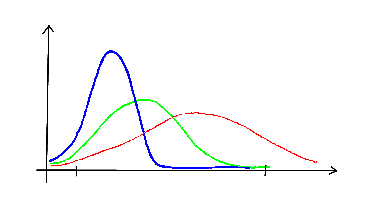
\includegraphics{zapfen.eps}}
\rput[t](1,0.3){400}
\rput[t](4.167,0.3){700}
\rput[t](5.5,0.5){$\lambda$}
\rput[bl](0.2,3){Empfindlichkeit -- $e_R(\lambda), e_G(\lambda), e_B(\lambda)$}
\end{pspicture}
\end{center}
Erregung der "`roten"' Zapfen bei einer Lichtquelle mit Intensitätsfunktion $f(\lambda)$
\[r = \int f(\lambda) \cdot e_R(\lambda)\ \mathrm{d} y \qquad f(\lambda)\]
analog "`grün"': $g = \int f(\lambda) \cdot e_G(\lambda)\ \mathrm{d} y$\\
analog "`blau"': $b = \int f(\lambda) \cdot e_B(\lambda)\ \mathrm{d} y$
\begin{itemize}
 \item Verschiedene Lichtquellen mit verschiednen spektraler Zusammensetzung erzeugen den gleichen Farbeindruck, wenn 	sie die gleichen $(r,g,b)$-Werte hervorbringen.
 \item Dreidimensionaler Farbraum, aber nicht alle $(r,g,b)$-Werte erreichbar\\
	(Wenn $g > 0 \Rightarrow r > 0$ oder $b > 0$, $(r,g,b) = (0,1,0)$ gibt es nicht)
 \item Wenn man $f(\lambda)$ mit einem Skalar $c > 0$ multipliziert, dann ändert sich nur die Helligkeit, nicht die
	Farbe. Entsprechend wird $(r,g,b)$ mit einem Skalar multipliziert.
 \item Normalisierung auf $r+b+g=1$ führt auf einen zweidimensionalen Farbraum, bei dem die Helligkeit konstant ist.
\end{itemize}
In der Computergrafik tut man so, als ob es nur \emph{drei} verschiedene Wellenlängen (Grundfarben) gibt: {\color{red}R}ot, {\color{green}G}rün und {\color{blue}B}lau
\begin{center}
\begin{pspicture}(0.5,0.5)(4,3)
	\psline[linecolor=red]{-*}(1,0)(1,2)\uput{2pt}[-90](1,0){\color{red}R}
	\psline[linecolor=green]{-*}(2,0)(2,2)\uput{2pt}[-90](2,0){\color{green}G}
	\psline[linecolor=blue]{-*}(3,0)(3,2)\uput{2pt}[-90](3,0){\color{blue}B}
	\psaxes[labels=none,ticks=none]{->}(0,0)(-0.1,-0.1)(4,2.5)
\end{pspicture}
\end{center}
\chapter{Rasterung von Strecken und Kreisen}
\section{Strecken}
\begin{itemize}
 \item Rendering pipeline wurde durchlaufen
 \item Koordinaten sind ganzzahlige Pixelkoordinaten
 \begin{center}
 \psset{unit=5mm}
 \begin{pspicture}(0,0)(6,8)
  \psgrid[gridlabels=0pt]
  \psframe*(1,1)(2,2)
  \psframe*(2,2)(3,3)
  \psframe*(3,3)(4,4)
  \psframe*(4,4)(5,5)
 \end{pspicture}
 \end{center}
\end{itemize}
 \paragraph*{Problemstellung} Gegeben sind zwei Punkte $p_1 = (x_1,y_1)$ und $p_2 = (x_2,y_2)$. Zeichne Strecke
	zwischen $p_1$ und $p_2$. $x_1, y_1, x_2, y_2$ sind ganzzahlig.
 \paragraph*{Vereinfachung} Strecken die durch den Nullpunkt gehen $(0,0), p_1 = (x_1, y_1)$
	\begin{itemize}
	\item Beschränkung auf Strecken im ersten Quadranten des Koordinatensystems. Alle anderen Strecken (im Quadranten
	II, III, IV) können durch Speigelung an $x$- oder $y$-Achse erzeugt werden
	\item Beschränkung aufersten Oktanten, alle anderen Strecken erhält man wie oben durch Vertauschen von $x$-
	 und $y$-Koordinate
	\end{itemize}
 \paragraph*{Vereinfachte Problemstellung}
	Gegeben ist ein Punkt $p_1 = (x_1,y_1)$ mit ganzzahligen Koordinaten. $x_1 \ge y_1, x_1 \ge 0, y_1 \ge 0$.
	Zeichne Strecke zwischen $(0,0)$ und $(x,y)$.
	\begin{align*}
	 \text{Geradengleichung: } g(x) &= \frac{y_1}{x_1} x & \text{Steigung: } m = \frac{y_1}{x_1}, 0 \le m \le 1
	\end{align*}
	 \begin{center}
	\psset{unit=5mm}
	\begin{pspicture}(-1,-1)(6,8)
		\psgrid[gridlabels=0pt]
		\psline[linecolor=red]{-}(0,0)(4,3)
		\psdot(0,0)
		\psdot(1,1)
		\psdot[dotstyle=o](2,1)
		\psdot(2,2)
		\psdot(3,2)
		\psdot[dotstyle=o](3,3)
		\psdot(4,3)
	\end{pspicture}
	\end{center}
\paragraph*{Idee} Werte für jeden Wert $i$ zwischen 0 und $x_1$ die Funktion $g$ aus. Runde das Ergebnis $g(i)$ und nimm
	diesen Wer als $j$-Wert
\begin{lstlisting}[mathescape=true]
double m = $y_1$/$x_1$;
for (i = 0; i <= $x_1$, i++) {
	j = round(i*m);	// auf- bzw. abrunden
	setPixel(i,j);
}
	\end{lstlisting}
	\begin{itemize}
	 \item erstetze \lstinline!j= round(i * m);! durch \lstinline!y=y+m_j; j = round(y);!
	 \item im $i$-ten Schritt $y_i = m \cdot i$
	 \item im $(i+1)$-ten Schritt $y_{i+1} = m \cdot (i+1)$
	 \item $y_{i+1} - y_i = m(i+1-1) = m$
	 \item $0 \le m \le 1 \Rightarrow y_{i+1} \le y_{i} + 1$
	 \item Wert von $j$ steigt pro Schleifendurchlauf um höchstens 1.
	\end{itemize}
	\begin{align*}
	 y_{i+1} &= y_i + m	& m &= \frac{y_1}{x_1}\\
	 j &= round(y_i)\\
	 y_i &= j + r_i & \text{Rest: } & -\frac{1}{2} \le r_i \le \frac{1}{2}\\
	 y_{i+1} &= y_i + m = j + \underbrace{r_i + m}_{r_{i+1}}
	\end{align*}
	\paragraph*{Algortithmus ohne Runden}
	\begin{lstlisting}[mathescape=true]
double m = $y_1$/$x_1$;
double r = 0;
int j = 0;
for (i = 0; i <= $x_1$; i+1) {
	r = r + m;	// y = y + m;
	if (r >= 1/2) {	// j = round(y)
		j = j+1,
		r = r - 1;
	}
	setPixel(i,j);
}
	\end{lstlisting}
z. B:
\begin{align*}
 y &= 0.6 & r_{alt} &= 0.6 \\
 y &= j_{alt} + r_{alt} & j_{neu} &= j_{alt} + 1\\
 y &= j_{neu} + r_{neu} & r_{neu} &= r_{alt} + 1 
\end{align*}
Immer noch ein Problem: \textbf{double}-Werte sind zu ungenau\\
Wir wissen, dass $x_1$ und $y_1$ ganzzahlig sind.\\
$\Rightarrow$ Multiplikation mit 2$x_1$ liefert \textbf{int}-Werte
\begin{lstlisting}[mathescape=true]
int m = 2*$y_i$;
int r = 0;
int j = 0;
setPixel(0,0);
for(int i = 1; i <= $x_1$; i++) {
	r = r + m;
	if (r >= $x_1$) {
		j = j+1;
		r = r - 2*$x_1$;
	}
	setPixel(i,j);
}
\end{lstlisting}
\[r_{i+1} + 2y_1 \ge x_1 \Leftrightarrow r \ge x_1 - 2 y_1\]
\begin{lstlisting}[mathescape=true]
int j = 0;
int m = 2*$y_1$;
int r = 2*$y_1$ - $x_1$;
int $c_1$ = m - 2*$x_1$;
int $c_2$ = m;
for (int i = 1; i <= $x_1$; i++) {
	if (r >= 0) {
		j++;
		r = r + $c_1$;
	} else {
		r = r + $c_2$;
	}
	setPixel(i,j);
}
\end{lstlisting}

\subsection{Bresenham-Algorithmus}
\begin{center}
 \psset{unit=3cm,arrows=-}
 % 6.1
 \begin{pspicture}(-0.5,-0,6)(1.5,1.5)
  \uput{2pt}[180](-0.5,0){$j_i$}
  \psline(-0.5,0)(1.5,0)
  \uput{2pt}[180](-0.5,1){$j_{i+1}$}
  \psline(-0.5,1)(1.5,1)
  \uput{2pt}[-90](0,-.5){$i$}
  \psline(0,-0.5)(0,1.5)
  \uput{2pt}[-90](1,-.5){$i+1$}
  \psline(1,-0.5)(1,1.5)
  \psframe[fillstyle=vlines](-0.1,-0.1)(0.1,0.1)
  \psline(-0.5,-0.25)(1.5,0.5)
  \psline[linecolor=red](-0.5,-0.375)(1.5,-0.1)
  \psline[linecolor=green](-0.5,0.25)(0.9,1.5)
  \psline(0.95,0.315)(1.05,0.315)
  \uput{3pt}[0](1.05,0.315){$q_{i+1}$}
  \psbrace[rot=180,ref=r,braceWidth=1pt](1,1)(1,0.315){$d_{i+1}''$}
  \psbrace[ref=l,braceWidth=1pt](1,0)(1,0.315){$d_{i+1}'$}
 \end{pspicture}
\end{center}
Wähle eine Spalte $i+1$ das Pixel, das am nächsten an $q_{i+1}$ liegt, also
\begin{align*}
 d_{i+1}' \le d_{i+1}'' &\Leftrightarrow \text{ wähle } j_{i+1} = j_i \\
 d_{i+1}'' < d_{i+1}' &\Leftrightarrow \text{ wähle } j_{i+1} = j_i + 1
\end{align*}
oder äquivalent
\begin{align*}
 d_{i+1}' - d_{i+1}''\le 0 &\Leftrightarrow j_{i+1} = j_i \\
 d_{i+1}' - d_{i+1}'' > 0 &\Leftrightarrow j_{i+1} = j_i + 1
\end{align*}
$y$-Koordinaten von $q_{i+1} \qquad \frac{y_1}{x_1} (i+1)$
\begin{align*}
 d_{i+1}' &= \frac{y_1}{x_1} (i+1)-j_i & d_{i+1}'' &= j_i + 1 - \frac{y_1}{x_1} (i+1)\\
 d_{i+1}' - d_{i+1}'' &= 2 \frac{y_1}{x_1} (i+1) - 2 j_i - 1 &&| \text{ multipliziere mit $x_1$}
\end{align*}
(ändert nichts an der Bedingung $\overset{<}{\underset{<}{=}}0$)\\
\hrulefill
Wir erhalten eine Fehler-/Entscheidungsvariable für $(i+1)$-te Spalte
\begin{align*}
 e_{i+1} &= x_i (d_{i+1}' - d_{i+1}'') = 2y_1(i+1) - 2 j_i x_1 - x_1\\
 e_{i+1} &\le 0\Leftrightarrow  j_{i+1}= j_i\\
 e_{i+1} &> 0 \Leftrightarrow  j_{i+1} = j_i +1
\end{align*}
Betrachte Differenz zwischen aufeinanderfolgenden Entscheidungsvariablen
\begin{align*}
 e_{i+1} - e_i &= \underline{2y_1(i+1)} - 2 j_i x_1 - \underline{x_1} - \underline{2y_1}i + 2j_{i-1}x_1
			+ \underline{x_1}\\
 e_{i+1} - e_i &= 2 y_1 - 2 x_1 \underbrace{(j_i - j_{i-1})}_{= \begin{cases}
                                                                 0, &\text{falls $e_i \le 0$}\\
								 1, & \text{falls $e_i > 0$}
                                                                \end{cases}
								}
\end{align*}
Also
\begin{align*}
 e_i > 0, j_i = j_{i-1} + 1 &\text{ und } e_{i+1} = e_i + 2y_1 - 2x_1 \\
 e_i \le 0, j_i = j_{i-1} &\text{ und } e_{i+1} = e_i + 2y_1
\end{align*}
Anfangswerte: $i=0, j_0 = 0,  e_1 = 2y_1 - x_1$

\pagebreak
\subsection{Midpoint Line Algorithmus}
\begin{center}
 \psset{unit=3cm,arrows=-}
 % 6.2
 \begin{pspicture}(-0.5,-0,6)(1.5,1.5)
  \uput{2pt}[180](-0.5,0){$j_i$}
  \psline(-0.5,0)(1.5,0)
  \uput{2pt}[180](-0.5,1){$j_{i+1}$}
  \psline(-0.5,1)(1.5,1)
  \uput{2pt}[-90](0,-.5){$i$}
  \psline(0,-0.5)(0,1.5)
  \uput{2pt}[-90](1,-.5){$i+1$}
  \psline(1,-0.5)(1,1.5)
  \psframe[fillstyle=vlines](-0.1,-0.1)(0.1,0.1)
  \psline(-0.5,-0.25)(1.5,0.5)
  \psline(0.95,0.5)(1.05,0.5)
  \uput{3pt}[180](0.95,0.5){$M_{i+1}$}
  \rput[l](2,0.5){$M_{i+1} = \vtwo{i+1}{j_i + \frac{1}{2}}$}
 \end{pspicture}
\end{center}
Wenn $M_{i+1}$ über der Strecke liegt $\Rightarrow$ wähle $j_{i+1} = j_i$
Wenn $M_{i+1}$ unter der Strecke liegt $\Rightarrow$ wähle $j_{i+1} = j_i +1$
\begin{align*}
 \text{Geradengleichung: } y = \frac{y_1}{x_1} x &\Leftrightarrow y_1x - x_1 y = 0 \\
 \text{$(x,y)$ liegt über der Geraden } \Leftrightarrow y > \frac{y_1}{x_1} x &\Leftrightarrow y_1x - x_1 y < 0 \\
 \text{$(x,y)$ liegt unter der Geraden } \Leftrightarrow  y < \frac{y_1}{x_1} x &\Leftrightarrow y_1x - x_1 y > 0 \\
\end{align*}
Setze $F(x,y) = x y_1 - x_1 y$, dann gilt also:
\begin{itemize}
 \item $(x,y)$ über Geraden $\Leftrightarrow F(x,y) < 0$
 \item $(x,y)$ auf Geraden $\Leftrightarrow F(x,y) = 0$
 \item $(x,y)$ unter Geraden $\Leftrightarrow F(x,y) > 0$
\end{itemize}
Entscheidungsvariable
\begin{align*}
 d_{i+1} = F(M_{i+1}) = (i+1)y_1-x_i\left(j_i + \frac{1}{2}\right) \le 0 &\Leftrightarrow j_{i+1} = j_i \\
 d_{i+1} = F(M_{i+1}) = (i+1)y_1-x_i\left(j_i + \frac{1}{2}\right) = 0 &\Leftrightarrow j_{i+1} = j_i + 1
\end{align*}
\begin{align*}
 d_{i+1} - d_i	&= y_1(i+1) - x_1\left(j_i + \frac{1}{2}\right)-y_1 i + x_1\left(j_{i+1}+\frac{1}{2}\right)\\
		&= y_1 - x_1 \underbrace{(j_i - j_{i-1})}_{= \begin{cases}
                                                                 0, &\text{falls $d_i \le 0$}\\
								 1, & \text{falls $d_i > 0$}
                                                                \end{cases}
								}\\
	d_1 &= y_1 - \frac{x_1}{2}
\end{align*}
Für Ganzzahligkeit multiplitziere mit 2
\begin{align*}
e_i = 2 d_i \Rightarrow e_{i+1} - e_i &= 2y_1 - 2x_1(j_i - j_{i-1})\\
		e_1 &= 2y_1 - x_1
\end{align*}

%% Rest s. Handybilder

\section{Kreise}
\begin{center}
	\psset{unit=0.5cm}
	\begin{pspicture}(0,0)(10,10)
		\psgrid[gridlabels=0pt]
		\psline[linecolor=gray,linestyle=dashed](8.5,5.5)(8.5,9.5)
		\psline[linecolor=gray,linestyle=dashed](7.5,6)(7.5,9.5)
		\psline[linecolor=gray,linestyle=dashed](6.5,6)(6.5,10)
		\psline[linecolor=gray,linestyle=dashed](6,6.5)(10,6.5)
		\psline[linecolor=gray,linestyle=dashed](5.5,8.5)(9,8.5)
		\psline[linecolor=gray,linestyle=dashed](5.5,7.5)(9.5,7.5)
		\psdot[linecolor=red](6.5,9.5)
		\psdot[linecolor=red](7.5,8.5)
		\psdot[linecolor=red](8.5,7.5)
		\psdot[linecolor=red](9.5,6.5)
		\psframe*[linecolor=red](0,3)(1,4)
		\psframe*[linecolor=red](0,4)(1,5)
		\psframe*[linecolor=red](1,2)(2,3)
		\psframe*[linecolor=red](2,1)(3,2)
		\pscircle(5,5){4.5}
		\psdot(5,5)
	\end{pspicture}
\end{center}

\paragraph*{Annahme}
	\begin{itemize}
	 \item	Radius $r$ ist ganzzahlig
	 \item	Mittelpunkt $(c_x,c_y)$ ist ein Gitterpunkt
	\end{itemize}	
	Kreisgleichung:
	\[(x-c_x)^2 + (y - c_y)^2 = r^2\]
	Betrachte den Fall, wo der Mittelpunkt (0,0) ist (anschließend alles um $(c_x,c_y)$ verschieben).
	Wir zeichnen den Bereich $x \ge 0, y \ge 0, y \ge x$ auf diesem Achtelkreis zeichnen wir auf jeder senkrechten
	Gittergeraden \emph{einen} Punkt.
	\begin{center}
	\psset{unit=0.3cm}
	\begin{pspicture}(-6,-6)(6,6)
		\rput[r](-12,5.5){Ausnutzung der Symmetrie:}
		\psgrid[gridlabels=0pt]
		\pscircle(0,0){6}
		\psdot(0,0)
		\psline(0,0)(5,5)
		\psline(0,0)(0,6)
		\psdot[linecolor=red](0,6)
		\psdot[linecolor=red](1,6)
		\psdot[linecolor=red](2,6)
		\psdot[linecolor=red](3,5)
		\psdot[linecolor=red](4,4)
		\psarc[linecolor=blue]{->}(0,0){6}{80}{90}
		\psarc[linecolor=blue]{<-}(0,0){6}{45}{60}
	\end{pspicture}
	\end{center}
	$x=i$ ist fest, Kreis verläuft zwischen $(i,j)$ und $(i,j+1)$.
	\begin{center}
	 \begin{pspicture}(0,0)(4,4)
		\psline(2,0)(2,4)
		\psline(1,0)(3,0)
		\psline(1,1)(3,1)
		\psline(1,2)(3,2)\uput{3pt}[0](3,2){$j$}
		\psline(1,3)(3,3)\uput{3pt}[0](3,3){$j+1$}
		\psline(1,4)(3,4)
		\psarc(0,-5){8}{60}{90}
	\end{pspicture}
	\end{center}
	Welchgen dieser beiden Punkte soll man auswählen?
	\begin{enumerate}
	 \renewcommand*\theenumi{(\arabic{enumi})}
	 \item	Wähle den Punkt, der kleineren \emph{Abstand} vom Kreis hat
	 \item	Berechne den Schnittpunkt mit der Geraden $x=i$ und $r$ und runde zum nächsten Gitterpunkt.
		\begin{itemize}
		 \item (Äquivalent: vergleiche den \emph{senkrechten Abstand} zum Kreis)
		 \item (Äquivalent: Liegt $(i, j+\frac{1}{2})$ über oder unter dem Kreisbogen?)
		\end{itemize}
	 \item	Wähle den Punkt der die \emph{Kreisgleichung} $x^2 + y^2 = r^2$ am besten erfüllt.
		\[|x^2 + y^2 - r^2| \to \mathrm{MIN}\]
	\end{enumerate}
	Für Geraden sind alle drei Bedingungen äquivalent\\
	Für (3). gibt es beliebig viele Varianten:
	\[\sqrt{x^2 + y^2} = r \Rightarrow |r - \sqrt{x^2 + y^2}| \to \mathrm{MIN} \text{ führt auf (1)}\]
	\[(x^2 + y^2)^2 = r^4 \Rightarrow |r^4 - (x^2 + y^2)^2| \to \mathrm{MIN} \text{ führt auf (1)}\]
	\begin{center}
	\begin{pspicture}(0,0)(4,4)
		\psdot(2,2.8)\pnode(2,2.8){i}
		\psline(0,1.5)(4,1.5)\psdot(2,1.5)\pnode(2,1.5){m}
		\psdot(2,0.2)\pnode(2,0.2){j}
		\psarc(0,0){3}{0}{90}
		\psline{<->}(2,0.2)(2.97,0.2)
		\nccurve[angleA=-60,angleB=60]{->}{i}{m}\naput{(2).}
		\nccurve[angleA=-120,angleB=120]{->}{m}{j}\nbput{(1).}
	\end{pspicture}
	\end{center}
\Satz	Wenn der Mittelpunkt $(c_x,c_y)$ und der Radius $r$ ganzzahlig sind, dann sind Bedingung (1),(2) und (3)
	äquivalent.\\
	\hrulefill
	Algebraische Formulierung von (1), (2), (3):
	\begin{itemize}
	 \item Punkt $(i,j+1)$ liegt außerhalb
		\[i^2 + (j + 1)^2 \ge r^2\]
	 \item Punkt $(i,j)$ liegt innerhalb
		\[i^2 + (j + 1)^2 < r^2\]
	\end{itemize}
	\newcommand{\glee}{\overset{>}{\underset{<}{=}}}
	\begin{enumerate}
	 \renewcommand*\theenumi{(\arabic{enumi})}
	 \item	$r-\sqrt{i^2+j^2} \glee \sqrt{i^2+(j+1)^2} - r$
	 \item	$i^2 + \left(j+\frac{1}{2}\right)^2 \glee r^2$
	 \item	$r^2 - (i^2 + j^2) \glee i^2+(j+1)^2 - r^2$
	\end{enumerate}
	\begin{align*}
	 (3) &\Longleftrightarrow 	& 2r^2	&\glee i^2 + j^2 + 2j + 1 + i^2 + j^2\\
		&		&	&= 2i^2 + 2j^2 + 2j + 1\\
	&\Longleftrightarrow	& i^2 + j^2 + j - r^2 + \frac{1}{2} &\glee 0 &&\Rightarrow\
		\text{"`="' kommt nicht vor für $i,j \in \mathbb{Z}$}\\
	 (2) &\Longleftrightarrow	& i^2 + j^2 + j + \frac{1}{4} - r^2 &\glee 0
	\end{align*}
	Für $i, j, r \in \mathbb{Z}$ sind (2) und (3) äquivalent:
	\begin{empheq}[box=\fbox]{align*}
		\overbrace{i^2 + j^2 + j - r^2}^{g(i,j+1),\ \text{s. Algorithmus}} &\ge 0 &&\Rightarrow\ \text{Zeichne $(i,j)$}\\
		 &\le -1 &&\Rightarrow\ \text{Zeichne $(i,j+1)$}
	\end{empheq}

	\paragraph*{Behauptung}
	\begin{enumerate}
	 \renewcommand*\theenumi{(\alph{enumi})}
	 \item $i^2 + \left(j + \frac{1}{2}\right)^2 \ge r^2 \Rightarrow \sqrt{i^2+(j+1)^2} - r > r - \sqrt{i^2+j^2}$
	 \item $i^2 + j^2 + j + \frac{1}{2} \le r^2 \Rightarrow \sqrt{i^2+(j+1)^2} - r < r - \sqrt{i^2+j^2}$
	\end{enumerate}
	Daraus folgt, dass Regel (1) mit den beiden anderen Regeln (2), (3) konsistent ist.\pagebreak
\Bew	(von (b).) Die Funktion $f(t) = \sqrt{t}$ ist fü $t > 0$ konkav
	\begin{center}
	\begin{pspicture}(0,-1)(4,4)
		\psarc(4,0){4}{90}{180}
		\psline{->}(0.5,0)(4,0)
		\psline(1,-0.1)(1,0.1)\uput{1pt}[-90](1,-0.1){$u$}
		\psline(2,-0.1)(2,0.1)\uput{1pt}[-90](2,-0.1){$\dfrac{u+v}{2}$}
		\psline(3,-0.1)(3,0.1)\uput{1pt}[-90](3,-0.1){$v$}
		\psline(1,0)(1,2.64)(3,3.87)(3,0)
		\psdot(1,2.64)\uput{1pt}[138.65](1,2.64){$f(u)$}
		\psdot(2,3.255)\rput[tl](4.5,2){$\dfrac{f(u)+f(v)}{2}$}
		\psline{->}(4.5,2)(2,3.255)
		\psdot(3,3.87)\uput{1pt}[104.49](3,3.87){$f(v)$}
	\end{pspicture}\\
	 (daraus folgt: $f\left(\dfrac{u+v}{2}\right) \ge \dfrac{f(u)+f(v)}{2}$)
	\end{center}
	Eine differenzierbare Funktion $f$ ist konkav $\Leftrightarrow$ $f'$ monoton fallen $\Leftrightarrow$ $f'' \le 0$
	\[f'(t) = \frac{1}{2 \sqrt{t}} \searrow\ \text{konkav}\]
	\begin{align*}
	 u &= i^2 + j^2\\
	 v &= i^2 + (j+1)^2 = i^2 + j^2 + 2j + 1\\
	 \frac{u+v}{2} &= i^2 + j^2 + j + \frac{1}{2}\\
	 r &\underset{\mathrm{N.V.}}{\ge} \sqrt{i^2 + j^2 + j + \frac{1}{2}} \ge \frac{1}{2} \left[\sqrt{i^2} + \sqrt{i^2+(j+1)^2}\right]\\
	 2r & \ge \sqrt{i^2+j^2} + \sqrt{i^2 + (j+1)^2}
	\end{align*}
\Bew	(von (a).) Funktion $h(y) = \sqrt{i^2 + y^2}$ ist \emph{konvex}
	\begin{align*}
	 h'(y) &= \frac{1 \cdot \cancel{2} y}{\cancel{2}\sqrt{i^2+y^2}} = \frac{1}{\sqrt{\frac{i^2}{y^2}+1}}
			\nearrow\text{ monoton wachsend}\\
	 g\left(\frac{u+v}{2}\right) &\le \frac{1}{2} (g(u) + g(v)) \qquad u = j, v = j+1\\
	 r^2 &\underset{\mathrm{N.V.}}{\le} \sqrt{i^2+\left(j+\frac{1}{2}\right)^2}
		\le \frac{1}{2}\left(\sqrt{i^2+j^2}+\sqrt{i^2 + (j+1)^2}\right)
	\end{align*}
\paragraph*{Algorithmus}
	beginnt mit $(0,r)$ und zeichnet Punkte von links nach rechts.
	\begin{itemize}
	 \item letzter gezeichneter Punkt $= (i-1,j)$
	 \item soll nächster $(i,j)$ oder $(i,j-1)$ gezeichnet werden?
		\begin{align*}
			g(i,j) &= i^2 + (j-1)^2 + (j-1) - r^2 = i^2 + j^2 - 2j \cancel{+ 1} + j \cancel{- 1} r^2\\
			g(i,j) &:= i^2 + j^2 - j - r^2 \begin{cases}
			                              \ge 0 &\Rightarrow\ \text{zeichne $(i, j-1)$}\\
			                              \le -1 & \Rightarrow\ \text{zeichne $(i, j)$}
			                             \end{cases}
		\end{align*}
		\begin{align*}
		 g(i+1,j) - g(i,j) &= (i+1)^2 - i^2 = 2i + 1\\
		 g(i,j-1) - g(i,j) &= (j-1)^2 - (j-1) - j^2 + j\\
				   &= j^2 - 2j + 1 - j + 1 - j^2 + j = -2j + 2
		\end{align*}
		\begin{center}
			\vspace{0.5cm}
			\begin{pspicture}(0,3)(3,6)
				\psgrid[gridlabels=0pt]
				\psline(0,3)(0,6)
				\rput[b](0,6){$(0,r)$}
				\rput[lb](2,5.5){$g(0,r) = -r$}
				\psline{->}(0,6)(1,6)
				\psline{->}(1,6)(1,5)
				\psline{->}(1,5)(2,5)
				\psline{->}(2,5)(2,4)
				\psdot[linecolor=red](0,6)
				\psdot[linecolor=red](1,6)
				\psdot[linecolor=red](1,5)
				\psdot[linecolor=red](2,5)
			\end{pspicture}
		\end{center}
	\end{itemize}
	\begin{lstlisting}[language=,keywords={loop,if,then, until},mathescape=true]
i := 0; j := r, g := -r; // Invariante: g = g(i,j)

loop
	SetPixel(i,j)
	g := g + 2i + 1; i := i + 1
	if g $\ge$ 0 then j := j - 1; g := g - 2j 
until j < i
	\end{lstlisting}

	\begin{lstlisting}[language=,mathescape=true]
SetPixel(c$_x$+i,$c_y$+j)
SetPixel(c$_x$+j,$c_y$+i)
SetPixel(c$_x$-i,$c_y$+j)
SetPixel(c$_x$-j,$c_y$+i)
SetPixel(c$_x$-i,$c_y$-j)
SetPixel(c$_x$-j,$c_y$-i)
SetPixel(c$_x$+i,$c_y$-j)
SetPixel(c$_x$+j,$c_y$-i)
	\end{lstlisting}
	Die Pixel in de n 4 Himmelsrichtungen werden doppelt gezeichnet.

\section{Schwachstellen der Rasterung (Aliasing)}
\begin{itemize}
 \item merkbare Sprünge bei fast achsenparallelen Geraden
	\begin{center}
	 \psset{unit=0.2cm}
	 \begin{pspicture}(0,0)(22,4)
	  \psgrid[gridlabels=0pt]
	  \psframe*(-2,1)(11,2)
	  \psframe*(11,2)(25,3)
	  \psline{->}(14,0)(11,2)
	  \rput[lt](14,0){deutlich sichtbarer Knick}
	 \end{pspicture}
	\end{center}
 \item unterschiedliche Helligkeitsverteilung in Abhängigkeit von der Steigung
	\begin{center}
	 \psset{unit=0.2cm}
	 \begin{pspicture}(0,0)(22,15)
	  \psgrid[gridlabels=0pt]
	  \psframe*(-2,13)(24,14)
	  \multirput(12,-1)(1,1){12}{
		\psframe*(0,0)(1,1)
	  }
	 \end{pspicture}
	\end{center}
	\begin{itemize}
	\item	horizontale/vertikale Linie hat 1 Pixel pro Längeneinheit
	\item	schräge Linie $(45^\circ)$ hat 1 Pixel pro $\sqrt{2}$ Längeneinheiten
	\end{itemize}
	$\Rightarrow$ schräge Linien erscheinen dünner
	\item	Buchstaben könne verschieden breit werden
	\begin{center}
		\psset{unit=0.5cm}
		\begin{pspicture}(0,0)(2,7)
			\rput[b](1,0){
				
\includegraphics[width=1cm,height=3.25cm]{bigi.eps}
			}
			\psgrid[gridlabels=0pt]
			\psdot(0,0)\psdot(0,4)
			\psdot(1,0)\psdot(1,1)\psdot(1,2)\psdot(1,3)\psdot(1,4)\psdot(1,6)
			\psdot(2,0)
		\end{pspicture}
		\hspace{2cm}
		\begin{pspicture}(0,0)(3,7)
			\rput[b](1.5,0){
				
\includegraphics[width=1cm,height=3.25cm]{bigi.eps}
			}
			\psgrid[gridlabels=0pt]
			\psdot(0,0)\psdot(0,4)
			\psdot(1,0)\psdot(1,1)\psdot(1,2)\psdot(1,3)\psdot(1,4)\psdot(1,6)
			\psdot(2,0)\psdot(2,1)\psdot(2,2)\psdot(2,3)\psdot(2,4)\psdot(2,6)
			\psdot(3,0)
		\end{pspicture}
	\end{center}

\end{itemize}
\paragraph*{Lösung (Antialiasing)}
	Verschiedene Graustufen für Pixel, statt nur schwarz und weiß



\section{Antialiasing}
verschiedene Ansätze:
\begin{enumerate}
 \item Betrachte den Bildpunkt als quadratische Fläche und nicht als Punkt, betrachte eine Kurve (1-dimensional) als Fläche (2-dimensional). z. B. Strecke als Rechtece
	\begin{center}
	 \psset{unit=0.5cm}
	 \begin{pspicture}(0,0)(5,5)
	  \psframe*(0,0)(5,5)
	  \rput{45}(2.5,2.5){
		\psframe*[linecolor=white](-2.5,-1.05)(2.5,-0.05)
	  }
	  \rput[r](-0.5,3){\rnode{49_l}{49\% weiß}}
	  \rput[l](5.5,2){\rnode{12_l}{12\% weiß}}
	  \psframe[fillstyle=hlines,hatchangle=60,linestyle=none,hatchsep=2pt](2,2)(3,3)
	  \pnode(2.5,2.4){49}
	  \psframe[fillstyle=hlines,hatchangle=60,linestyle=none,hatchsep=2pt](4,2)(5,3)
	  \pnode(4.2,2.8){12}
	  \psgrid[gridcolor=gray,gridlabels=0pt]
	  \ncline[linecolor=gray]{->}{49_l}{49}
	  \ncline[linecolor=gray]{->}{12_l}{12}
	 \end{pspicture}
	\end{center}
	Pixel wird entsprechend hell- oder dunkelgrau gefärbt. (im Allgemeinen als proportionale Mischung aller Farben,
	die im Pixelquadrat vorkommen).
	\begin{center}
		\psset{unit=0.5cm}
		\begin{pspicture}(0,0)(5,5)
			\rput{45}(2.5,2.5){
				\psframe*(-2.5,0)(2.5,1)
			}
			\rput{-45}(2.5,2.5){
				\psframe*[linecolor=red](-2.5,0)(2.5,-1)
			}
			\psframe[fillstyle=hlines,hatchangle=60,linestyle=none,hatchcolor=gray,hatchsep=2pt](2,2)(3,3)
			\psgrid[gridcolor=gray,gridlabels=0pt]
		\end{pspicture}
	\end{center}
	Aufwendig zu rechnen.
 \item Supersampling: Man rechnet mit einer höheren Pixeldichte als tatsächlich vorhanden.
	\begin{center}
		\psset{unit=0.75cm}
		\begin{pspicture}(0,0)(5,4)
			\rput{30}(2.2,2.5){
				\psframe*(-2.5,-1.1)(2.5,-0.1)
			}
			\psgrid[gridcolor=comment,gridlabels=0pt]
			\multirput(0,0)(0,1){4}{
				\multirput(0,0)(1,0){5}{
					\multirput(0.167,0.167)(0,0.333){3}{
						\multirput(0,0)(0.333,0){3}{
							\psdot[dotstyle=x,linecolor=gray]
						}
					}
				}
			}
			\pnode(3.5,1.5){1}
			\pnode(2.5,2.5){5}
			\rput[r](-0.5,3){\rnode{5l}{$\dfrac{5}{9}$ weiß}}
			\rput[l](5.5,2){\rnode{1l}{$\dfrac{1}{9}$ weiß}}
			\ncline[linecolor=gray]{->}{1l}{1}
			\ncline[linecolor=gray]{->}{5l}{5}
		\end{pspicture}
	\end{center}
	die verfeinerten Pixel werden "`binär"' zugeordnet (in Fläche und außerhalb) und entsprechend gesetzt.
	Die Werte der tatsächlichen Pixel ergeben sich als Mittelwert der in ihnen enthaltenen verfeinerten Pixel.
 \item Glättung:
	\paragraph*{Idee}
	\begin{center}
	 \begin{pspicture}(0,0)(10,1.4)
		\psset{linewidth=0.1mm}
		\multirput(0,1)(0.197,-0.034){10}{
			\pscircle(0,0){0.41}
			\pscircle(0,0){0.25}
			\pscircle(0,0){0.17}
			\pscircle(0,0){0.13}
			\pscircle(0,0){0.11}
			\psdot[dotsize=0.2cm](0,0)
		}
	 \end{pspicture}
	\end{center}
	Helligkeitswerte "`strahlen"' auf die Nachbarn ab.
	\begin{enumerate}
	\item berechne die Pixelweite zunächst ohne Antialiasing.
	\item Verteile die Helligkeit von jedem Pixel auf seinen Nachbarn nach einem festen Schema.
	\end{enumerate}
	\begin{center}
		\psset{unit=0.6cm,gridlabels=0pt}
		\begin{pspicture}(0,0)(3,3)
			\rput[r](-2,3){z. B.}
			\psgrid
			\rput(0.5,2.5){$\tfrac{1}{36}$}\rput(1.5,2.5){$\tfrac{4}{36}$}\rput(2.5,2.5){$\tfrac{1}{36}$}
			\rput(0.5,1.5){$\tfrac{4}{36}$}\rput(1.5,1.5){$\tfrac{16}{36}$}\rput(2.5,1.5){$\tfrac{4}{36}$}
			\rput(0.5,0.5){$\tfrac{1}{36}$}\rput(1.5,0.5){$\tfrac{4}{36}$}\rput(2.5,0.5){$\tfrac{1}{36}$}
		\end{pspicture}
	\end{center}
\end{enumerate}
3. lässt sich auch mit 2. kombinieren

\chapter{Helligkeit und Farbe in der Computergrafik}
\section{Helligkeit}
\Defi Helligkeit in der schwarz/weiß-Grafik bezeichnet einen Grauwert auf der Skala zwischen schwarz und weiß
	\begin{align}
	 \text{schwarz } &= 0, & \text{weiß } &= 1\\
	 \text{oder schwarz } &= 0, & \text{weiß } &= 25 \qquad \text{(8-Bit-Integer)}
	\end{align}
\paragraph*{Problem} tatsächliche Mischung 50\% weiß und 50\% schwarz $\rightarrow$ sehr hellesgrau
\paragraph*{Weber-Fechner'sches Gesetz} beschreibt die Nichtlinearität der Sinneswahrnehmungen (für Optik und
	Akustik gleichermaßen). Vergrößerung der Energie um einen \emph{konstanten Faktor} wird als Vergrößerung des Reizes in \emph{konstanten Schritten} wahrgenommen.
\Bsp	Eine Vergrößerung von 10 auf 12 Energieeinheiten wird genauso groß wahrgenommen wie eine Vergrößerung von
	5000 auf 6000.
\Bsp	Lautstärke wir in deziBel (dB) gemessen: Logarithmus aus der Schallenergie (oder Druck?). (Logarithmus aus
	konstanten Faktoren konstante Differenzen).
\Bsp	Eine Oktave in der Musik (z. B. Abstand zwischen tiefen C und hohen C) entspricht einer Verdoppelung der
	Schallfrequenz.
\begin{center}
	\begin{pspicture}(0,0)(5,3)
	 \psaxes{->}(0,0)(0,0)(5,3)
	 \psplot{0}{5}{2.7*x^3/125}
	 \rput(0,3.2){Intensität der Lichtbestrahlung}
	 \rput[l](5.2,0){Grauwert des Pixels}
	 \pstextpath[l](0,0){\psplot[linestyle=none]{1}{5}{2.7*x^3/125+0.1}}{Funktion der Form $y = x^\gamma$}
	\end{pspicture}
	% 8.7 
\end{center}
"`$\gamma$-Korrektur"', wird vom Bildschirm bzw. von der Grafikkarte automatisch durchgeführt.

\section{Additive Farbsysteme}
\subsection{Das RGB-Farbsystem}
In der Computergrafik geht man von einem 3-Komponenten-Modell aus: Farbe ist aus 3 Grundfarben zusammengemischt
\begin{center}
 {\color{red}rot (R)}, {\color{green}grün (G)}, {\color{blue}blau (B)}
\end{center}
(In Wirklichkeit: unendlich viele Grundfarben, für jede sichtbare Wellenlänge eine)
\begin{center}
 \psset{unit=0.25cm}
 \begin{pspicture}(0,0)(2.5,0.5)
  \multirput(0.25,0)(1.5,0){2}{
	\SpecialCoor
	\psdot[linecolor=red](0.36;-150)
	\psdot[linecolor=green](0.36;-30)
	\psdot[linecolor=blue](0.36;90)
	\pspolygon[linewidth=0.1mm](-0.75,-0.433)(0,0.866)(0.75,-0.433)
  }
  \multirput{180}(1,0.433)(1.5,0){2}{
	\SpecialCoor
	\psdot[linecolor=red](0.36;-150)
	\psdot[linecolor=green](0.36;-30)
	\psdot[linecolor=blue](0.36;90)
	\pspolygon[linewidth=0.1mm](-0.75,-0.433)(0,0.866)(0.75,-0.433)
  }
 \end{pspicture}
\end{center}
Auf einem Bildschirm sind Lichtpunkte (Phosphore) in drei Farben R, G, B nahe aneinander gitterförmig angeordnet,
Die Bildpunkte werden unabhängig von einander angesteuert.\\
Eine Farbe in der Computergrafik ist durch 3 RGB-Werte zwischen 0 und 1 (0,1, ..., 255) charakterisiert. 24 bit pro Pixel, $2^24 \approx 16$ Millionen Farben
\begin{center}
 \begin{tabular}{ll}
  \textbf{Farbe}	& $\boldsymbol{(r,g,b)}$\\
  rot			& (1,0,0)\\
  grün			& (0,1,0)\\
  blau			& (0,0,1)\\
  gelb (Y)		& (1,1,0)\\
  magenta (M)		& (1,0,1)\\
  cyan (C)		& (0,1,1)\\
  schwarz (K)		& (0,0,0)\\
  weiß			& (1,1,1)\\
  Grauwerte		& $(x,x,x)$ alle drei Werte sind gleich
 \end{tabular}\\
 \psset{unit=4cm,xMin=0,xMax=1.5,yMin=0,yMax=1.5,zMin=0,zMax=1.5,Alpha=60,Beta=20,linecolor=yellow,nameX=$r$,nameY=$g$,nameZ=$b$}
 \begin{pspicture}(-1,-0.5)(1,1.5)
  \pstThreeDCoor[linecolor=black]
  \pstThreeDBox(0,0,0)(1,0,0)(0,1,0)(0,0,1)
  \pstThreeDLine(0,0,0)(1,1,1)
  \pstThreeDPut(1,1,1){weiß}
  \pstThreeDPut(0.5,0.5,0.5){\rput{50}(0,0){Grauachse}}
  \pstThreeDPut(0,0,0){K}
  \pstThreeDPut(1,0,0){R}
  \pstThreeDPut(1,1,0){Y}
  \pstThreeDPut(1,0,1){M}
  \pstThreeDPut(0,1,0){G}
  \pstThreeDPut(0,1,1){C}
  \pstThreeDPut(0,0,1){B}
 \end{pspicture}\\
 Farbwürfel $[0,1]^3$
\end{center}
\begin{itemize}
 \item Das RGB-System ist für die intuitive Behandlung von Farben nicht geeignet
 \item die Grauwerte bilden die Grauachse $K$-Weiß im Farbwürfel.
 \item die übrigen Ecken bilden das Farbsechseck RYGCBM. Auf diesem Sechseck liegen die "`reinsten"'/"`stärksten"'
	Farben, alle anderen Farben kann man durch beimischen von Grau konstruieren.
\end{itemize}
\begin{center}
	\definecolor{this}{rgb}{0.25,0.75,0.25}
 \psset{unit=4cm,xMin=0,xMax=1.5,yMin=0,yMax=1.5,zMin=0,zMax=1.5,Alpha=60,linecolor=gray,Beta=20,nameX=$r$,nameY=$g$,nameZ=$b$}
 \begin{pspicture}(-1,-0.5)(1,1.5)
  \pstThreeDCoor[linecolor=black]
  \pstThreeDPut(0.5,0.5,0.75){$\vthree{\frac{1}{2}}{\frac{1}{2}}{\frac{1}{2}}$}
  \pstThreeDPut(0.25,0.75,0.5){$\vthree{\frac{1}{4}}{\frac{3}{4}}{\frac{1}{4}}$}
  \pstThreeDBox(0,0,0)(1,0,0)(0,1,0)(0,0,1)
  \pstThreeDLine(0,0,0)(1,1,1)
  \pstThreeDLine[linecolor=red](1,0,0)(1,1,0)(0,1,0)(0,1,1)(0,0,1)(1,0,1)(1,0,0) % HSV-Effekt?
  \pstThreeDPut(1,0.5,0){$\vthree{1}{g}{0}$}
  \pstThreeDPut(0,0.5,1){$\vthree{0}{g}{1}$}
  \pstThreeDPut(0.5,1,0){$\vthree{r}{1}{0}$}
  \pstThreeDPut(0.5,0,1){$\vthree{r}{0}{1}$}
  \pstThreeDPut(1.1,0,0.5){$\vthree{1}{0}{b}$}
  \pstThreeDPut(0,1.1,0.5){$\vthree{0}{1}{b}$}
  \pstThreeDPut(1,1,1){W}
  \pstThreeDPut(0,0,0){K}
  \pstThreeDPut(1,0,0){R}
  \pstThreeDPut(1,1,0){Y}
  \pstThreeDPut(1,0,1){M}
  \pstThreeDPut(0,1,0){G}
  \pstThreeDPut(0,1,1){C}
  \pstThreeDPut(0,0,1){B}
  \pstThreeDDot(0.5,0.5,0.5) % mit Koord beschriften
  \pstThreeDLine(0.5,0.5,0.5)(0,1,0) % mit Koord beschriften
  \pstThreeDPut(0,1,-0.25){$\vthree{0}{1}{0}$}
  \pstThreeDDot[linecolor=this](0.25,0.75,0.25) % mit Koord beschriften
 \end{pspicture}
\end{center}
Diese "`stärksten Farben"' sind die Farben din mindestens eine Komponente 0 und mindestens eine Komponente 1 haben
(Farben ohne Grau/Weiß/Schwarz-Anteil).

\subsection{Farbsechseck bzw. Farbkreis}
\begin{center}
 \begin{pspicture}(0,0)(4,4)
  \rput(2,2){
	\SpecialCoor
	\psline[linecolor=gray](1.85;40)(0,0)(2;90)
	\pspolygon(2;90)(2;30)(2;-30)(2;-90)(2;-150)(2;150)
	\psarc[linecolor=blue]{<-}(0,0){1.2}{100}{80} % HSV-Effekt?
	\psdot[linecolor=red](2;90)\uput{0.4cm}[-90](2;90){$0^\circ$}
	\psdot[linecolor=yellow](2;30)\uput{0.4cm}[-150](2;30){$60^\circ$}
	\psdot[linecolor=green](2;-30)\uput{0.4cm}[150](2;-30){$120^\circ$}
	\psdot[linecolor=cyan](2;-90)\uput{0.4cm}[90](2;-90){$180^\circ$}
	\psdot[linecolor=blue](2;-150)\uput{0.4cm}[30](2;-150){$240^\circ$}
	\psdot[linecolor=magenta](2;150)\uput{0.4cm}[-30](2;150){$300^\circ$}
	\rput(1;65){$40^\circ$}
  }
 \end{pspicture}
 \hspace{2cm}
 \begin{pspicture}(0,0)(4,4)
  \rput(2,2){
	\SpecialCoor
	\psline[linecolor=red](2;40)(0,0)(2;90)
	\pscircle(0,0){2}	% HSV-Effekt
	\psdot[linecolor=red](2;90)\uput{0.2cm}[90](2;90){$0^\circ$}
	\psdot[linecolor=yellow](2;30)\uput{0.2cm}[30](2;30){$60^\circ$}
	\psdot[linecolor=green](2;-30)\uput{0.2cm}[-30](2;-30){$120^\circ$}
	\psdot[linecolor=cyan](2;-90)\uput{0.2cm}[-90](2;-90){$180^\circ$}
	\psdot[linecolor=blue](2;-150)\uput{0.2cm}[-150](2;-150){$240^\circ$}
	\psdot[linecolor=magenta](2;150)\uput{0.2cm}[150](2;150){$300^\circ$}
	\rput(1;65){$40^\circ$}
  }
 \end{pspicture}
\end{center}
\begin{itemize}
 \item Die Punkte auf diesem Sechseck werden häufig durch einen Winkel ($0^\circ-360^\circ$) parametrisiert.
 \item Startpunkt willkürlich (R = $0^\circ$, Y = $60^\circ$, ...)
 \item Dieser Parameter heißt "`Farbton"', "`Unbuntart"' (engl. \textit{hue} (H)). 
\end{itemize}
\begin{align*}
 40^\circ\ \text{entspricht dann } & \frac{1}{3} \cdot \mathrm{R} + \frac{2}{3} \cdot \mathrm{Y} \left(\frac{1}{3} \cdot 0^\circ
	+ \frac{2}{3} \cdot 60^\circ\right)\\
	&= \frac{1}{3} \cdot (1,0,0) + \frac{2}{3} \cdot (1,1,0) = \left(1, \frac{2}{3}, 0\right)
\end{align*}
Wir erhalte ein neues Farbsystem HSV

\subsection{Andere Farbsysteme}
\subsubsection{HSV-System}
\begin{description}
 \item[hue] (Farbton) $0^\circ \le H \le 360^\circ$
 \item[saturation] (Sättigung) $0 \le S \le 1$
 \item[value] ($\approx$ Helligkeit) $0 \le B \le 1$
\end{description}
$V = 1$ sind die Farben auf den drei Deckseiten des Würfels: mindest einer der drei Werte ist 1
\[max(r,g,b) = 1\]
\begin{center}
	\definecolor{azure}{rgb}{0.25,0.75,0.25}
 \psset{unit=4cm,xMin=0,xMax=1.5,yMin=0,yMax=1.5,zMin=0,zMax=1.5,Alpha=60,linecolor=gray,Beta=20,nameX=$r$,nameY=$g$,nameZ=$b$}
 \begin{pspicture}(-1,-0.5)(1,1.5)
  \pstThreeDCoor[linecolor=black]
  \pstThreeDBox(0,0,0)(1,0,0)(0,1,0)(0,0,1)
  \pstThreeDLine(0,0,0)(1,1,1)
  \pstThreeDSquare[fillstyle=vlines](1,0,0)(0,0,1)(0,1,0)
  \pstThreeDSquare[fillstyle=vlines](0,0,1)(1,0,0)(0,1,0)
  \pstThreeDSquare[fillstyle=vlines](0,1,0)(0,0,1)(1,0,0)
  \pstThreeDPut(1,1,1){W}
  \pstThreeDPut(0,0,0){K}
  \pstThreeDPut(1,0,0){R}
  \pstThreeDPut(1,1,0){Y}
  \pstThreeDPut(1,0,1){M}
  \pstThreeDPut(0,1,0){G}
  \pstThreeDPut(0,1,1){C}
  \pstThreeDPut(0,0,1){B}
 \end{pspicture}
\end{center}
Umrechnung HSV $\to$ RGB:
\begin{align*}
 \vthree{r''}{g''}{b''} &\text{sei die reine Farbe, die $H$ entspricht.}\\
 \vthree{r'}{g'}{b'} &= S \vthree{r''}{g''}{b''} + (1-S) \vthree{1}{1}{1}\\
 \text{Ergebnis } \vthree{r}{g}{b} &= V \vthree{r'}{g'}{b'}
\end{align*}
Umrechnung RGB $\to$ HSV
\begin{center}
 \psset{unit=3cm,Alpha=80,Beta=15}
 \begin{pspicture}(-0.2,-0.4)(1,1)
  \pstThreeDBox(0,0,0)(1,0,0)(0,1,0)(0,0,1)
  \pstThreeDSquare[fillstyle=vlines,hatchangle=0,hatchsep=1pt,hatchcolor=gray](0.7,0,0)(0,0,0.3)(0,0.3,0)
  \pstThreeDSquare[fillstyle=vlines,hatchangle=-60,hatchsep=1pt,hatchcolor=gray](0.7,0,0.3)(0.3,0,0)(0,0.3,0)
  \pstThreeDSquare[fillstyle=vlines,hatchangle=-60,hatchsep=1pt,hatchcolor=gray](0.7,0.3,0)(0,0,0.3)(0.3,0,0)
  \pstThreeDPut(1.04,-0.04,-0.04){$K$}
  \pstThreeDPut(-0.04,1.04,1.04){$W$}
  \pstThreeDPut(0.7,0.15,0.4){$V=0{,}3$}
 \end{pspicture}
 \hspace{2cm}
 \begin{pspicture}(-0.2,-0.4)(1,1)
  \pstThreeDBox(0,0,0)(1,0,0)(0,1,0)(0,0,1)
  \pstThreeDLine[fillstyle=vlines](1,0,0)(0.5,0,1)(0,1,1)(1,0,0)
  \pstThreeDPut(1.04,-0.04,-0.04){$K$}
  \pstThreeDPut(-0.04,1.04,1.04){$W$}
  \pstThreeDPut(0.5,1.4,0.5){$H$ konst.}
 \end{pspicture}\\
 \psset{unit=3cm,Alpha=100,Beta=20}
 \begin{pspicture}(-0.2,-0.4)(1,1.2)
  \pstThreeDLine[linecolor=gray](0.2,0.8,1)(1,0,0)(0,1,0.8)
  \pstThreeDLine[linecolor=gray](0.2,1,0.8)(1,0,0)(0,0.8,1)
  \pstThreeDLine[linecolor=gray](0,0.8,0.8)(1,0,0)(0.2,1,1)
  \pstThreeDSquare[linecolor=gray](0,0.8,0.8)(0,0,0.2)(0,0.2,0)
  \pstThreeDBox(0,1,0)(1,0,0)(0,-1,0)(0,0,1)
  \pstThreeDSquare[linecolor=gray](0,0.8,1)(0.2,0,0)(0,0.2,0)
  \pstThreeDSquare[linecolor=gray](0,1,0.8)(0.2,0,0)(0,0,0.2)
  \pstThreeDPut(1.04,-0.04,-0.04){$K$}
  \pstThreeDPut(-0.04,1.04,1.04){$W$}
  \pstThreeDPut(0.5,1.4,0.5){$S = 0{,}2$}
 \end{pspicture}
\end{center}
\begin{align*}
 V &= \max(r,g,b)\\
 \vthree{r'}{g'}{b'} = \vthree{r}{g}{b} \cdot \frac{1}{V}\\
 S &= 1 - \min(r',g',b')\\
 \rnode{v''}{\vthree{r''}{g''}{b''}} &= \left[\vthree{r'}{g'}{b'}-(1-S)\vthree{1}{1}{1}\right] \cdot \frac{1}{S}
\end{align*}
\rnode{rF}{reine Farbe} $\rightarrow$ Umwandlung in $H$ \nccurve[angleA=45]{->}{rF}{v''}
\begin{center}
 \psset{unit=3cm,Alpha=100,Beta=20}
  \begin{pspicture}(-0.2,-0.4)(1,1.6)
  \pstThreeDBox(0,1,0)(1,0,0)(0,-1,0)(0,0,1)
  \pstThreeDLine(0,1,1)(0.5,0,1)
  \pstThreeDDot(0,1,1)
  \pstThreeDDot(0.25,0.5,1)
  \pstThreeDDot(0.5,0,1)
  \pstThreeDPut(1.04,-0.04,-0.04){$K$}
  \pstThreeDPut(-0.04,1.04,1.04){$W$}
  \pstThreeDPut(0.25,0.5,1.4){$\vthree{r'}{g'}{b'}$}
 \end{pspicture}
\end{center}
$\vthree{r''}{g''}{b''}$ ist tatsächlich eine reine Farben
\begin{enumerate}
 \item Wir wissen $\max(r',g',b') = 1$ z. B. $r' = 1$
	\[r'' = [1-(1-S)1] \cdot \frac{1}{S} = S \frac{1}{S} = 1\]
 \item Nehmen wir nun an $(r',g',b') = g' = 1-S$
	\[g'' = [g'-(1-S)1] \cdot \frac{1}{S} = [-1 + S + 1 - S] \frac{1}{S} = 0\]
\end{enumerate}
Für $V = 0$ setze $S, H$ beliebig.\\
Für $V \neq 0$, $S = 0$, setze $H$ beliebig.
\begin{center}
 \psset{xunit=1.5,yunit=4.5}
 \begin{pspicture}(0,0)(6,2)
 \rput(0,-1){
  \psframe*[linecolor=red](0.3,2)(0.7,2.8)
  \psframe*[linecolor=green](1.3,2)(1.7,2.2)
  \psframe*[linecolor=blue](2.3,2)(2.7,2.5)
  \psaxes[labels=y,ticks=y](0,2)(0,3)(3,2)
  \uput{5pt}[-90](0.5,2){$r$}
  \uput{5pt}[-90](1.5,2){$g$}
  \uput{5pt}[-90](2.5,2){$b$}
  
  \psline{|<->|}(4.75,2.2)(4.75,2.8)\uput{1mm}[0](4.75,2.5){$S \cdot V$}
  \psline{|<->|}(4.75,2)(4.75,2.2)\uput{1mm}[0](4.75,2.1){$(1-S) \cdot V$}
  
  \psline[linestyle=dashed](3,2)(4.6,2)
  \psline[linestyle=dashed](3.7,2.8)(4.6,2.8)
  \psline[linestyle=dashed]{->}(0,2.8)(3.5,2.8)\uput*{1mm}[0](3.5,2.8){$\max \to V$}
  \psline[linestyle=dashed](3.7,2.2)(4.6,2.2)
  \psline[linestyle=dashed]{->}(0,2.2)(3.5,2.2)\uput*{1mm}[0](3.5,2.2){$\min$}
  \psline{|<->|}(-0.1,2.2)(-0.1,2.8)
  \pnode(-0.1,2.5){H_arrow}
  
  \psbrace(6,2.8)(6,3){schwarz = $1 - V$}
  \psbrace(6,2.2)(6,2.8){reine Farbe}
  \psbrace(6,2)(6,2.2){weiß = $V \cdot (1 - S)$}
 }
 \psset{yunit=0.6}
 \pnode(-0.3,0.95){H}
 \psaxes[labels=y,ticks=y](0,0)(0,0)(3,1)
 \psframe*[linecolor=red](0.3,0)(0.7,1)
 \psframe*[linecolor=green](1.3,0)(1.7,0)
 \psframe*[linecolor=blue](2.3,0)(2.7,0.5)
 
 \rput(4,0.8){\rnode{H_label}{\LARGE $H$}}
 \pnode(1.5,0.5){H_middle}
 
 \nccurve[angleA=-140,angleB=140]{->}{H_arrow}{H}
 
 \nccurve[angleA=-160,angleB=20]{->}{H_label}{H_middle}
 \end{pspicture}
\end{center}
Nachteil:
\begin{description}
 \item $\mathrm{R} = (1,0,0)$
 \item $\mathrm{Y} = (1,1,0)$
 \item $\mathrm{W} = (1,1,1)$
\end{description}
haben denselben $V$-Wert.

\subsubsection{HSL-System}
\begin{description}
 \item[hue] (Farbton) $0^\circ \le H \le 360^\circ$
 \item[saturation] (Sättigung) $0 \le S \le 1$
 \item[lightness] (oder "`luminance"') $L = \tfrac{1}{2}$ enthält das reine Farbensechseck und den Graupunkt
	$\left(\tfrac{1}{2},\tfrac{1}{2},\tfrac{1}{2}\right)$
\end{description}
\begin{center}
 \psset{Alpha=150,Beta=20}
 \begin{pspicture}(0,-1)(2,4)
  \pstThreeDLine[linewidth=2pt](0,0,2)(2,0,2)(2,0,0)(2,2,0)(0,2,0)(0,2,2)(0,0,2)
  \pstThreeDDot(1,1,1)
  \pstThreeDLine(1,1,1)(0,0,2)
  \pstThreeDLine(1,1,1)(2,0,2)
  \pstThreeDLine(1,1,1)(2,0,0)
  \pstThreeDLine(1,1,1)(2,2,0)
  \pstThreeDLine(1,1,1)(0,2,0)
  \pstThreeDLine(1,1,1)(0,2,2)
 \end{pspicture} \hspace{2cm}
 \begin{pspicture}(0,-1)(2,4)
  \pstThreeDLine[linewidth=2pt](1.5,0,0)(3,1.25,1.2)(3,3.75,0.8)(1.5,5,2)(0,3.75,0.8)(0,1.25,1.2)(1.5,0,0)
  \pstThreeDDot(1.5,2.5,1)
  \pstThreeDLine(1.5,2.5,1)(1.5,0,0)
  \pstThreeDLine(1.5,2.5,1)(3,1.25,1.2)
  \pstThreeDLine(1.5,2.5,1)(3,3.75,0.8)
  \pstThreeDLine(1.5,2.5,1)(1.5,5,2)
  \pstThreeDLine(1.5,2.5,1)(0,3.75,0.8)
  \pstThreeDLine(1.5,2.5,1)(0,1.25,1.2)
 \end{pspicture} \hspace{4cm}
 \begin{pspicture}(-1,-2)(1,2)
  \psset{linecolor=gray}
  \pspolygon(0,2)(-1,0)(0,-2)(1,0)
  \psellipse(0,0)(1,0.5)
  \psline(0,2)(0,-2)
  \psdot(0,0)
  \uput{3pt}[45](0,0){$\left(\tfrac{1}{2},\tfrac{1}{2},\tfrac{1}{2}\right)$}
  \uput{3pt}[180](-1,0){$L=\frac{1}{2}$}
  \uput{3pt}[180](0,2){$L=1$}
  \uput{3pt}[180](0,-2){$L=-1$}
 \end{pspicture}
\end{center}
Umrechnung HSL $\to$ RGB:
\begin{align*}
 \vthree{r''}{g''}{b''} &\text{sei die reine Farbe, die $H$ entspricht.}\\
 \vthree{r'}{g'}{b'} &= S \vthree{r''}{g''}{b''} + (1-S) \vthree{1}{1}{1}\\
 \text{Für } 0 \le L \le \frac{1}{2}: \vthree{r}{g}{b} &= \vthree{r'}{g'}{b'} \cdot 2L\\
 \text{Für } \frac{1}{2} \le L \le 1: \vthree{r}{g}{b} &= \vthree{r'}{g'}{b'} \cdot (2-2L) +
			\vthree{1}{1}{1} \cdot (2L - 1)
\end{align*}
\begin{center}
 \psset{unit=3cm,Alpha=200,Beta=10}
  \begin{pspicture}(-0.2,-0.2)(1,1.4)
  \pstThreeDLine[fillstyle=solid,fillcolor=gray](0.15,0.15,0.15)(0.3,0,0)(0.3,0.3,0)(0.15,0.15,0.15)
  \pstThreeDLine[fillstyle=solid,fillcolor=gray](0.15,0.15,0.15)(0.3,0.3,0)(0,0.3,0)(0.15,0.15,0.15)
  \pstThreeDLine[fillstyle=solid,fillcolor=gray](0.15,0.15,0.15)(0,0.3,0)(0,0.3,0.3)(0.15,0.15,0.15)
  \pstThreeDLine[fillstyle=solid,fillcolor=gray](0.15,0.15,0.15)(0,0.3,0.3)(0,0,0.3)(0.15,0.15,0.15)
  \pstThreeDLine[fillstyle=solid,fillcolor=gray](0.15,0.15,0.15)(0,0,0.3)(0.3,0,0.3)(0.15,0.15,0.15)
  \pstThreeDLine[fillstyle=solid,fillcolor=gray](0.15,0.15,0.15)(0.3,0,0.3)(0.3,0,0)(0.15,0.15,0.15)
  \pstThreeDDot(0.15,0.15,0.15)
  \pstThreeDBox(1,1,0)(-1,0,0)(0,-1,0)(0,0,1)
  \pstThreeDPut(-0.1,-0.1,-0.1){$K$}
  \pstThreeDPut(1.1,1.1,1.1){$W$}
 \end{pspicture}
 \hspace{2cm}
 \begin{pspicture}(-0.2,-0.2)(1,1.4)
  \pstThreeDLine[linecolor=gray](0.6,0.4,0.4)(0.6,0.6,0.4)(0.4,0.6,0.4)(0.4,0.6,0.6)(0.4,0.4,0.6)(0.6,0.4,0.6)(0.6,0.4,0.4)
  \pstThreeDLine[linecolor=gray](0,0,0)(0.6,0.4,0.4)(1,1,1)(0.4,0.6,0.6)(0,0,0)
  \pstThreeDLine[linecolor=gray](0,0,0)(0.6,0.6,0.4)(1,1,1)(0.4,0.4,0.6)(0,0,0)
  \pstThreeDLine[linecolor=gray](0,0,0)(0.4,0.6,0.4)(1,1,1)(0.6,0.4,0.6)(0,0,0)
  \pstThreeDBox(1,1,0)(-1,0,0)(0,-1,0)(0,0,1)
  \pstThreeDPut(-0.1,-0.1,-0.1){$K$}
  \pstThreeDPut(1.1,1.1,1.1){$W$}
  \pstThreeDPut(1.6,0,0.5){$S = 0{,}2$ in HSL}
 \end{pspicture}
\end{center}
$S = 1$ Farben auf allen 6 Seitenflächen des Würfels



\section{Subtraktive Farbmischung (z. B. beim Drucken)}
3 Grundfarben
\begin{description}
 \item $C = $ cyan, $B, G$ wird durchgelassen, $R$ wird absorbiert
 \item $M = $ magenta, $B, R$ wird durchgelassen, $G$ wird absorbiert
 \item $Y = $ gelb, $R, G$ wird durchgelassen, $B$ wird absorbiert
\end{description}
$C + M$ nur Blau bleibt übrig\\
$C + M + Y = $ schwarz

\subsection{CMY-System}
$0 \le C, M, Y \le 1$
\begin{align*}
 C &:= 1 - R\\
 M &:= 1 - G\\
 Y &:= 1 - B
\end{align*}
\begin{center}
  \psset{xunit=1.5,yunit=3}
 \begin{pspicture}(0,0)(3,1)
  \psframe*[linecolor=red](0.3,0)(0.7,0.6)
  \psframe*[linecolor=green](1.3,0)(1.7,0.8)
  \psframe*[linecolor=blue](2.3,0)(2.7,0.5)
  \psaxes[labels=y,ticks=y](0,0)(0,1)(3,0)
  \uput{5pt}[-90](0.5,0){$R$}
  \uput{5pt}[-90](1.5,0){$G$}
  \uput{5pt}[-90](2.5,0){$B$}  
 \end{pspicture}
 \hspace{2cm}
 \begin{pspicture}(0,0)(3,1)
  \psframe*[linecolor=cyan](0.3,0)(0.7,0.4)
  \psframe*[linecolor=magenta](1.3,0)(1.7,0.2)
  \psframe*[linecolor=yellow](2.3,0)(2.7,0.5)
  \psaxes[labels=y,ticks=y](0,0)(0,1)(3,0)
  \uput{5pt}[-90](0.5,0){$C$}
  \uput{5pt}[-90](1.5,0){$M$}
  \uput{5pt}[-90](2.5,0){$Y$}  
 \end{pspicture}
\end{center}

\subsection{CMYK-System (Vierfarbdruck)}
Zusätzlich $K = $schwarz. (Das Schwarz von $K$ wird dunkler als von $C + M + Y$ oder um Druckfarbe zu sparen.)
\begin{align*}
 K' &:= \min(C, M, Y)\\
 C' &:= C - K'\\
 M' &:= M - K'\\
 Y' &:= Y - K'
\end{align*}
(möglichst viel Farbe durch $K$ ersetzen)

\section{Gängige Farbdarstellung heutzutage}
\begin{itemize}
 \item 8 Bit pro Farbkanal $(r,g,b)$ ... 24 Bit pro Bildpunkt\\
	$\Rightarrow 2^{24} = 16\ \text{Mio. Farben}$ (True Color)
 \item 4-Kanal-Darstellung $(r, g, b, \alpha)$
	$\alpha$ ist für Transparenz:
	\begin{itemize}
	 \item $\alpha = 0...$ durchsichtig; Farbe wird vom Hintergrund genommen,
	 \item $\alpha = 1...$ Farbe wird von $(r, g, b)$ bestimmt
	 \item $0 < \alpha < 1...$ teilweise transparent
	\end{itemize}
	$\rightarrow$ 32 bit pro Pixel
\end{itemize}

\subsection{Farbpaletten}
Es wird nicht für jeden Pildpunkt eine unabhängige Farbe gespeichert (24 Bit) sonder ein Index in einer Tabelle (8 Bit,
= Farbpaletten).
\begin{center}
 \psset{unit=0.75cm}
 \begin{pspicture}(0,-0)(8,6)
  \psgrid[gridlabels=0pt,subgriddiv=10,gridcolor=lgray,gridwidth=0.1pt,subgridwidth=0.1pt]
  \fnode[framesize=0.1 0.1](6.25,4.35){pix}
  \uput{3pt}[180](0,3){600}
  \uput{3pt}[-90](4,0){800}
 \end{pspicture}\hspace{2cm}
 \begin{tabular}{|r|l|}
  \hline
  \tiny 0 & \\
  \tiny 1 & \\
  & \\
  & \\
  \hline
  \Rnode[vref=2pt]{tab}{} & Farbe 24 Bit \\
  \hline
  & \\
  & \\
  & \\
  & \\
  \hline
  \tiny 255 & \\
  \hline
 \end{tabular}
 \nccurve[angleA=0,angleB=180]{->}{pix}{tab}
 \vspace{3pt}
\end{center}
Animation ganz einfach und schnell möglich.
\begin{center}
 \begin{pspicture}(0,0)(2.25,1)
  \psframe(0,0)(2.25,1)
  \pspolygon(0,0)(0.25,0)(0.5,0.5)(0.25,1)(0,1)
  \pspolygon(0.25,0)(0.5,0.5)(0.25,1)(0.75,1)(1,0.5)(0.75,0)
  \pspolygon(0.75,0)(1,0.5)(0.75,1)(1.25,1)(1.5,0.5)(1.25,0)
  \pspolygon(1.25,0)(1.5,0.5)(1.25,1)(1.75,1)(2,0.5)(1.75,0)
  \pspolygon(1.75,0)(2.25,0)(2.25,1)(1.75,1)(2,0.5)
  \rput(0.25,0.5){\small 0}
  \rput(0.75,0.5){\small 1}
  \rput(1.25,0.5){\small 2}
  \rput(1.75,0.5){\small 3}
  \rput(2.125,0.5){\small 4}
 \end{pspicture}\\[1em]
 \begin{tabular}{r|l|}
	\tiny 0	& \texttt{\textcolor{red}{\#FF0000}}\\
		& \texttt{\#000000}\\
		& \texttt{\#000000}\\
		& \texttt{\#000000}\\
	\tiny 4	& \texttt{\#000000}
 \end{tabular}
 \hspace{2cm}
 \begin{tabular}{r|l|}
	\tiny 0	& \texttt{\textcolor{red}{\#FF0000}}\\
		& \texttt{\textcolor{red}{\#FF0000}}\\
		& \texttt{\#000000}\\
		& \texttt{\#000000}\\
	\tiny 4	& \texttt{\#000000}
 \end{tabular}
\end{center}
Heutzutage eher historisch.

\chapter{Beleuchtung}
Standardfall:
\begin{center}
 \psset{Alpha=50}
 \begin{pspicture}(-3,-0.4)(3,3)
  % http://commons.wikimedia.org/wiki/File:Bulbgraph.svg
  \pstThreeDPut(3,-3,3){
\includegraphics[height=1cm]{bulb.eps}}
  \pstThreeDSquare(-1,-2,0)(2,0,0)(0,3,0)
  \pstThreeDLine[linecolor=yellow]{->}(3,-3,3)(0,0,0)
  \pstThreeDBox[linestyle=dotted](1,-2,1)(1,0,0)(0,1,0)(0,0,1)
  \pstThreeDPut(2.3,-2,0.5){Schatten}
  \pstThreeDLine[linecolor=yellow]{->}(0,0,0)(-3,3,3)
  \pstThreeDBox[linestyle=dotted](-1.5,1.5,1.5)(1,0,0)(0,1,0)(0,0,1)
  \rput[l](3,1){Verdeckung durch Hindernis}
  \rput[l](1.6,0){Fläche (Oberfläche eines Objekts)}
  \pstThreeDDot(-3,3,3)
  \pstThreeDPut(-3,3.6,3){Auge}
 \end{pspicture}

\end{center}

In Wirklichkeit sehr komplex, in der Computergrafik aber eher selten angewandt:
\begin{center}
 \psset{Alpha=50}
 \begin{pspicture}(-3,-0.4)(3,4)
  % http://commons.wikimedia.org/wiki/File:Bulbgraph.svg
  \pstThreeDPut(3,-3,3){
\includegraphics[height=1cm]{bulb.eps}}
  \pstThreeDSquare(-1,-2,0)(2,0,0)(0,3,0)
  \pstThreeDSquare(-2,-3,0.5)(0,3,0)(0,0,2)
  \pstThreeDLine[linecolor=yellow]{->}(3,-3,3)(0,0,0)
  \pstThreeDLine[linecolor=yellow]{->}(3,-3,3)(-2,-1.5,1.5)
  \pstThreeDLine[linecolor=yellow]{->}(3,-3,3)(2,-1.5,1.5)
  \pstThreeDLine[linecolor=yellow]{->}(2,-1.4,1.5)(-2,-1.4,1.5)
  \pstThreeDLine[linecolor=yellow]{->}(-2,-1.6,1.5)(2,-1.6,1.5)
  \pstThreeDLine[linecolor=yellow]{->}(0,0,0)(-3,3,3)
  \pstThreeDLine[linecolor=yellow]{->}(-2,-1.5,1.5)(0,0,0)
  \pstThreeDLine[linecolor=yellow]{->}(0,0,0)(2,-1.5,1.5)
  \pstThreeDSquare(2,-3,0.5)(0,3,0)(0,0,2)
  \pstThreeDDot(-3,3,3)
  \pstThreeDPut(-3,3.6,3){Auge}
 \end{pspicture}
\end{center}

Beleuchtung ist wichtig um einen räumlichen Eindruck zu erzeugen
\begin{center}
 \definecolor{darkgreen}{rgb}{0,0.75,0}
 \definecolor{darkergreen}{rgb}{0,0.5,0}
 \begin{pspicture}(7,3)
  \pspolygon[fillstyle=solid, fillcolor=green,linestyle=none](0,0.5)(1.5,0)(1.5,2)(0,2.5)
  \psline[fillstyle=solid, fillcolor=darkergreen,linestyle=none](1.5,0)(3,0.5)(3,2.5)(1.5,2)
  \psline[fillstyle=solid, fillcolor=darkgreen,linestyle=none](1.5,3)(0,2.5)(1.5,2)(3,2.5)

  \rput[bl](4,0){
	\pspolygon[fillstyle=solid, fillcolor=green,linestyle=none](0,0.5)(1.5,0)(3,0.5)(3,2.5)(1.5,3)(0,2.5)
  }
 \end{pspicture}
\end{center}
Flächenbeschaffenheit:\\
\begin{tabular}{rlr}
 1) & diffuse Reflexion; "`sieht aus allen Richtungen gleich aus"' &\Rnode[vref=10pt]{dR}{}\\
 \\
 2) & spiegelndes Reflexion;&\pnode{sR}
\end{tabular}
\psbrace(sR)(dR){treten auch kombiniert auf}

\section{Diffuse Reflexion}\label{sec:diffuse_refl}
	$L, N, A$ sind Einheitsvektoren:
	\begin{align*}
	 N... &\text{Normalvektor der Fläche}\\
	 L... &\text{Vektor zur Lichtquelle}\\
	 A... &\text{Vektor zum Auge}\\
	 \theta... &\text{Einfallswinkel (zwischen $L$ und $N$)}
	\end{align*}
	\begin{center}
	 \psset{Alpha=50,unit=2,Beta=10}
	 \begin{pspicture}(-2,-0.5)(2,1.2)
	  \pstThreeDSquare(-1,-1,0)(2,0,0)(0,2,0)
	  \pstThreeDSquare(-0.15,-0.15,0)(0.3,0,0)(0,0.3,0)
	  \pstThreeDLine{->}(0,0,0)(0,0,1)
	  \pstThreeDPut(0,0,1.11){$N$}
	  \pstThreeDLine{->}(0,0,0)(0,-0.707,0.707)
	  \pstThreeDPut(0,-0.8,0.8){$L$}
	  \pstThreeDLine{->}(0,0,0)(0,0.707,0.707)
	  \pstThreeDPut(0,0.8,0.8){$A$}
	  \pstThreeDCircle[beginAngle=0,endAngle=-45,arrows=<->](0,0,0)(0,0,0.5)(0,0.5,0)
	  \pstThreeDPut(0,-0.17,0.34){$\theta$}
	 \end{pspicture}
	\end{center}
	Wie erscheint ein Punkt (Flächenstück) für das Auge?
	\[I = \text{Intensität}\]
	zusätzliche Daten:
	\begin{align*}
	 r_L... &\text{Abstand zur Lichtquelle}\\
	 I_L... &\text{Intensiät der Lichtquelle}\\
	 K_D... &\text{diffuser Reflexionskoeffizient der Fläche}
	\end{align*}
	\begin{center}
	\begin{minipage}{0.95\linewidth}
	Abhängigkeit von $\theta$ (\textbf{Lampert'sches Gesetz})\label{lambert}
	\[I = \cos \theta \cdot (\dots) \qquad \cos \theta \langle N, L \rangle\]
	\begin{center}
		\psset{unit=2}
		 \begin{pspicture}(0,0.5)(2,4)
		 \psdot(0.75,4)
		 \psline[linecolor=yellow](0.25,2.5)(0.75,4)(1.25,2.5)
		 \psline(0,2.7)(1.5,2.7)
		 \psdot(0.75,2.7)
		 \psline{->}(0.75,2.7)(1.2,2.7)
		 \uput{3pt}[-90](0.975,2.7){$r$}
		 \psframe(0,0.5)(1.5,2)
		 \pscircle[linecolor=yellow](0.75,1.25){0.45}
		 \psline{->}(0.75,1.25)(1.2,1.25)
		 \uput{3pt}[-90](0.975,1.25){$r$}
		 \psdot(0.75,1.25)
		 \end{pspicture}
		 \hspace{2cm}
		 \begin{pspicture}(0,0.5)(2,4)
		 \psdot(0.75,4)
		 \psline[linecolor=yellow](0.25,2.5)(0.75,4)(1.25,2.5)
		 \psline(0,2.5)(1.5,3)
		 \psdot(0.75,2.75)
		 \psline[linestyle=dotted](0.75,2.75)(1.15,2.75)
		 \psline{->}(0.75,2.75)(1.135,2.875)
		 \uput{3pt}[-90](0.975,2.7){$r$}
		 \psframe(0,0.5)(1.5,2)
		 \psellipse[linecolor=yellow](0.75,1.25)(0.55,0.45)
		 \psline{->}(0.75,1.25)(0.75,1.7)
		 \uput{3pt}[180](0.75,1.475){$r$}
		 \psline{->}(0.75,1.25)(1.3,1.25)
		 \uput{3pt}[-90](1.025,1.25){$\frac{r}{\cos \theta}$}
		 \psdot(0.75,1.25)
		 \end{pspicture}
		 \hspace{1cm}
		 \psset{unit=0.4}
		 \begin{pspicture}(0,0)(4,3)
		  \rput[bl](0,6){
			\psline(0,0)(4,3)(4,0)
			\uput{4pt}[126.87](2,1.5){$\dfrac{r}{\cos \theta}$}
			\psline[linestyle=dotted](0,0)(4,0)
			\uput{4pt}[-90](2,0){$r$}
			\psline(3.5,0)(3.5,0.5)(4,0.5)
			\dotnode[dotsize=2px](3.75,0.25){T}
			\psarc(0,0){1.5}{0}{36.87}
			\SpecialCoor
			\rput(1;18.435){$\theta$}
			\rput[r](4,-0.75){\rnode{S}{annähernd $90^\circ$}}
			\ncline{->}{S}{T}
		  }
		 \end{pspicture}
	\end{center}
	\textbf{Begründung:}
	Die Menge an Lichtenergie, die auf eine Fläche auftrifft, hängt vom räumlichen Winkel ab, unter dem die Fläche von der
	Lichtquelle aus erscheint.
	\begin{center}
	 \psset{unit=2cm}
	 \begin{pspicture}(0,-0.4)(1.570796327,1)
	  \psaxes[xunit=1.570796327,trigLabels,showorigin=false,labels=y](0,0)(0,0)(1.2,1)
	  \psplot{0}{1.570796327}{cos(x)}
	  \rput[t](1.570796327,-0.12){$\dfrac{\pi}{2}$}
	 \end{pspicture}
	\end{center}
	Die gleiche Menge an Licht, die vorher auf eine Fläche von $r^2 \pi$ gefallen ist, fällt jetzt auf eine
	Fläche von $r \cdot r \dfrac{1}{\cos \theta} \cdot \pi ...$, pro Flächeneinheit kommt um den Faktor
	$\cos \theta$ beim Auge weniger an.
	\end{minipage}
	\end{center}
	$\Rightarrow$ $I$ hängt \emph{nicht von $A$} ab. (Das ist spezifisch für die diffuse Reflexion)\\
	Abstand zur Lichtquelle: Physikalisch $\dfrac{1}{r_L^2}$ (liefert in der Praxis zu starke
	Kontraste)
	\begin{center}
		\psset{Alpha=50}
		\begin{pspicture}(-3,-0.4)(1,4)
			% http://commons.wikimedia.org/wiki/File:Bulbgraph.svg
			\pstThreeDSquare(2,-4.5,4.5)(2,0,0)(0,0,-2)
			\pstThreeDPut(3,-3,3){
\includegraphics[height=1cm]{bulb.eps}}
			\pstThreeDSquare(-1,-2,0)(2,0,0)(0,3,0)
			\pstThreeDLine[linecolor=yellow]{->}(3,-3,3)(0,0,0)
			\pstThreeDLine[linecolor=yellow]{->}(3,-3,3)(3,-4.5,3.5)
			\pstThreeDPut(3,-3.75,3.25){5 cm}
			\pstThreeDPut(1.5,-1.5,1.5){2 m}
		\end{pspicture}
	\end{center}
	Mit der Formel $\dfrac{1}{r_L^2}$ würde das einen Faktor 400 bedeuten.
	Man nimmt stattdessen eine Formel der Gestalt:
	\[\frac{1}{C_1 + C_2 r_L^2 + C_3 r_L^2} \qquad \text{für passende Konstanten $C_1, C_2, C_3$}\]
	\begin{itemize}
	 \item Formel für diffuse Reflexion
		\[\boxed{I = I_L \frac{1}{C_1 + C_2 r_L + C_3 r_L^2} \cos \theta \cdot K_D} \qquad \left(0 \le \theta \le \frac{\pi}{2}\right)\]
	 \item Diese Formel wird für jede Farbkomponente {\color{red}R}, {\color{green}G}, {\color{blue}B} angewandt
		\begin{align*}
		I^{\color{red}R} &= I^{\color{red}R}_L \frac{1}{C_1 + C_2 r_L + C_3 r_L^2} \cos \theta \cdot K^{\color{red}R}_D\\
		I^{\color{green}G} &= I^{\color{green}G}_L \frac{1}{C_1 + C_2 r_L + C_3 r_L^2} \cos \theta \cdot K^{\color{green}G}_D\\
		I^{\color{blue}B} &= I^{\color{blue}B}_L \frac{1}{C_1 + C_2 r_L + C_3 r_L^2} \cos \theta \cdot K^{\color{blue}B}_D
		\end{align*}
	 \item In Wirklichkeit müsste man das für jede Wellenlänge $\lambda$ getrennt ausrechnen.
		\[\cos \theta \text{ durch } \max(0,\langle N, L \rangle)\]
	 \item Für unendlich ferne \emph{Lichtquellen} lässt man den Term $\dfrac{1}{C_1 + C_2 r_L + C_3 r_L^2}$ weg.
		$I_L$ hat eine andere Bedeutung. $L$ ist dann konstant.

	 \item Man betrachtet auch Umgebungslicht. Es kommt aus allen Richtungen gleich stark.
		\[ I = I_{L,E} \cdot K_E \qquad \text{für $R,G,B$ getrennt}\]
	 \item Um die Helligkeit eines Flächenstücks (in $R$, $G$, $B$) zu berechnen, werden die Ergebnisse der verschiedenen
		Lichtquellen und der diffusen Beleuchtung aufsummiert.
	\end{itemize}





\section{Spiegelnde Reflexion}
\begin{center}
 \psset{Alpha=175,Beta=10}
 \begin{pspicture}(-2,0)(4,4)
  \pstThreeDSquare(0,0,0)(4,0,0)(0,4,0)
  \pstThreeDPut(3,2,3){\rnode{A}{Auge}}
  \pstThreeDPut(-1,2,3){
\includegraphics[width=0.6cm]{bulb.eps}}
  \pstThreeDNode(2,2,0){mitte}
  \ncline[linestyle=dashed]{mitte}{A}
  \pstThreeDLine{->}(2,2,0)(1,2,1)\pstThreeDPut(0.8,2,1.2){$L$}
  \pstThreeDLine[linestyle=dashed]{->}(2,2,0)(3,2,1)\pstThreeDPut(3.2,2,1.2){$L'$}
  \pstThreeDLine{->}(2,2,0)(2.447,2,1.342)\pstThreeDPut(2.3,2,1.6){$A$}
  \pstThreeDLine{->}(2,2,0)(2,2,1.414)\pstThreeDPut(2,2,1.6){$N$}
  \pstThreeDCircle[beginAngle=0,endAngle=-45](2,2,0)(0,0,0.8)(1.2,0,0)
  \pstThreeDPut(1.8,2,0.5){$\theta$}
  \pstThreeDCircle[beginAngle=0,endAngle=45](2,2,0)(0,0,0.8)(2.8,0,0)
  \pstThreeDPut(2.2,2,0.5){$\theta$}
  \pstThreeDCircle[beginAngle=18.43,endAngle=45](2,2,0)(0,0,1)(3,0,0)
  \pstThreeDPut(2.7,2,1.1){$\alpha$}
 \end{pspicture}
\end{center}

$L'$ ist der an $N$ gespiegelte Vektor, die der "`idealen Spiegelung"'
\[\alpha = \measuredangle(A,L')\]
Modell von \textsc{Bui-Tong Phong}: Intensität ist proportional zu $\cos^n \alpha$
\begin{center}
 \psset{xunit=4.712,yunit=3,showorigin=false,algebraic=false,labels=none}
 \begin{pspicture}(-1.1,-0.1)(1.1,1.2)
  \psaxes{<->}(0,0)(-1.1,-0.1)(1.1,1.2)
  \psplot[unit=3,linecolor=red]{-1.57}{1.57}{x 180 mul 3.141592654 div cos}
  \psplot[unit=3,linecolor=red]{-1.57}{1.57}{x 180 mul 3.141592654 div cos 10 exp}
  \psplot[unit=3,plotpoints=500,linecolor=red]{-1.57}{1.57}{x 180 mul 3.141592654 div cos 50 exp}
  \psplot[unit=3,plotpoints=500,linecolor=red]{-1.57}{1.57}{x 180 mul 3.141592654 div cos 1000 exp}
  \rput[bl](0.1,1.1){$\cos^n \alpha$}
  \rput[tc](1,-0.2){$\frac{\pi}{2}$}
  \rput[tc](-1,-0.2){$-\frac{\pi}{2}$}
  \psset{unit=3}
  \uput{5pt}[45](0.785,0.707){$n = 1$}
  \uput{5pt}[28.05](0.393,0.452){$n = 10$}
  \uput{5pt}[28.05](0.2,0.3){$n = 50$}
  \uput{5pt}[20](0.05,0.1){$n = \infty$}
 \end{pspicture}
\end{center}
\begin{center}
 \psset{Alpha=170,Beta=20}
 \begin{pspicture}(-2,-3)(4,4.5)
  \pstThreeDPut(-1,2,-3){\rput{180}{
\includegraphics[width=0.6cm]{bulb.eps}}}
  \pstThreeDLine[linecolor=yellow](-1,2,-3)(2,2,0)
  \pstThreeDSquare(0,0,0)(4,0,0)(0,4,0)
  \pstThreeDPut(5,2,3){\rnode{A}{Auge}}
  \pstThreeDPut(-1,2,3){
\includegraphics[width=0.6cm]{bulb.eps}}
  \pstThreeDLine[linecolor=yellow](-1,2,3)(2,2,0)
  \pstThreeDNode(2,2,0){mittig}
  \pstThreeDNode(2.433,2.25,0){30}
  \pstThreeDNode(2.433,1.75,0){90}
  \pstThreeDNode(2,2.5,0){150}
  \pstThreeDNode(1.567,2.25,0){210}
  \pstThreeDNode(1.567,1.75,0){270}
  \pstThreeDNode(2,1.5,0){330}
  \ncline[linecolor=red]{A}{mittig}
  \pstThreeDDot(2,2,0)
  \ncline[linewidth=0.2px]{A}{30}
  \ncline[linewidth=0.2px]{A}{90}
  \ncline[linewidth=0.2px]{A}{150}
  \ncline[linewidth=0.2px]{A}{210}
  \ncline[linewidth=0.2px]{A}{270}
  \ncline[linewidth=0.2px]{A}{330}
  \rput(5,0){\rnode{a0}{$\alpha = 0$}}
  \pstThreeDNode(2.5,2,0.5){a0_a}
  \ncline{->}{a0}{a0_a}
  \rput(2,2){$\alpha > 0$}
 \end{pspicture}
 \hspace{2cm}
 \begin{pspicture}(0,0)(4,4.5)
  \rput(2,4.25){Bild aus Sicht des Auges}
  \psframe(0,0)(4,4)
  \rput{180}(2,2){
\includegraphics[width=0.35cm]{bulb.eps}}
  \pspolygon(0.5,1)(1.5,2.5)(2.5,2.5)(3.5,1)
 \end{pspicture}

\end{center}
Formel für spiegelnde Reflexion:
\[I^X = I^X_L \cdot \frac{1}{C_0 + C_1 r + C_2 r^2} \cdot K_S \cdot \cos^n \alpha,\qquad X = R, G, \text{ oder } B\]
\begin{align*}
	I_L...\ & \text{Intensität der Lichtquelle $(I_L^R, I_L^G, I_L^B)$}\\
	\frac{1}{C_0 + C_1 r + C_2 r^2}...\ & \text{Abhängigkeit von der Entfernung der Lichtquelle}\\
	K_S...\ & \text{spiegelnde Reflexionskoeffizient \emph{unabhängig von der Farbe!}}\\
	n...\ & \text{Exponent: gibt an wie glatt die Spiegelung ist}\\
	\frac{1}{C_0 + C_1 r + C_2 r^2}...\ & \text{Abhängigkeit von der Entfernung der Lichtquelle}\\
	I^R, I^G, I^B...\ & \text{Ergebnis-Intensität aus Sicht des Auges}\\
\end{align*}
\begin{center}
 \begin{pspicture}(0,0)(3,2.5)
  \rput[l](3,2){$\|L\| = \|N\| = \|A\| = 1$}
  \psline{->}(1.5,0)(1.5,2)
  \uput{3pt}[90](1.5,2){$N$}
  \psline{->}(1.5,0)(3.232,1)
  \uput{3pt}[30](3.232,1){$L'$}
  \psline{->}(1.5,0)(-0.232,1)
  \uput{3pt}[150](-0.232,1){$L$}
  \psline[linestyle=dashed](-0.232,1)(3.232,1)
  \psline{->}(1.5,0)(-0.232,1)
  \uput{3pt}[0](1.5,0.5){$L_0$}
  \psline{->}(1.45,1.1)(-0.232,1.1)
  \psline{->}(1.55,1.1)(3.232,1.1)
 \end{pspicture}
\end{center}
\begin{align*}
 L_0&...\ \text{Projektion von $L$ auf $N$}\\
    &= \langle L, N \rangle \cdot N\\
 L' &= -(L-L_0) + L_0 = 2L_0 - L, \|L'\|=1\\
 \cos \alpha &= \langle A, L' \rangle =  \langle A, 2L_0 \rangle -  \langle A, L \rangle\\
  &= 2  \langle L, N \rangle \langle N, A \rangle -  \langle A, L \rangle\\
	&= \cos \alpha
\end{align*}
\paragraph*{Näherungsmodell} (einfacher zu rechnen)\\
$H$ der Vektor, der symmetrisch zwischen $A$ und $L$ liegt.
\begin{align*}
 H_0 &= A + L & H &= \frac{H_0}{\|H_0\|} 
\end{align*}
Statt $\cos \alpha$ nimmt man $\cos \beta, \beta = \measuredangle(H,N)$
\[\cos \beta = \langle H, B \rangle \qquad \beta = 0 \Leftrightarrow \alpha = 0\]
\begin{center}
 \psset{unit=3cm}
 \begin{pspicture}(-1,0)(1,1.1)
  \psline(-1,0)(1,0)
  \SpecialCoor
  \psline{->}(0,0)(1;90)
  \uput{3pt}[90](1;90){$N$}
  \psline{->}(0,0)(1;160)
  \uput{3pt}[160](1;160){$L$}
  \psline[linestyle=dashed]{->}(0,0)(1;20)
  \uput{3pt}[20](1;20){$L'$}
  \psline{->}(0,0)(1;60)
  \uput{3pt}[60](1;60){$A$}
  \psline{->}(0,0)(1;110)
  \uput{3pt}[110](1;110){$H$}
  \psline(0.25;135)(0.35;135)
  \psarc(0,0){0.3}{110}{160}
  \psline(0.2;85)(0.3;85)
  \psarc(0,0){0.25}{60}{110}
  \psarc(0,0){0.8}{90}{110}
  \uput{3pt}[100](0.8;100){$\beta$}
  \psarc(0,0){0.8}{20}{60}
  \uput{3pt}[40](0.8;40){$\alpha$}
 \end{pspicture}
\end{center}
$\beta = \frac{\alpha}{2}$, wenn $L, N, A$ in einer Ebene liegen. Im Raum ist das nicht immer der Fall.

\section{Gesamtbeleuchtung}
\begin{itemize}
 \item mehrere Lichtquellen an bestimmten Orten (bzw. aus bestimmten Richtungen) mit Intensität $I_L^R, I_L^G, I_L^B$
 \item eine diffuse Lichtquelle mit Intensität $I_D^R, I_D^G, I_D^B$
\end{itemize}
Für jede Fläche:
\begin{itemize}
 \item diffuse Reflexionskoeffizienten $K_D^R, K_D^G, K_D^B$
 \item spiegelnde Reflexionskoeffizienten $K_S$, Exponent $n$
 \item möglicherweise eine Eigenleuchtintensität $I_E^R, I_E^G, I_E^B$ (z. B. Leuchtschirm, glühendes Ofenrohr,
									flächig leuchtende Lichtquelle)
\end{itemize}
Für jedes Flächenstück addiert man alle Beleuchtungskomponennten zusammen (falls die Fäche sichtbar vom Auge ist).
\begin{align*}
 I^R &= \sum \text{diffuse Reflexionen von allen Lichtquellen, die das Flächenstück beleuchten.} \\
	& \qquad + I_D^R \cdot K^R \\
	& \qquad + \text{spiegelnde Reflexionen von allen Lichtquellen, die das Flächenstück beleuchten.} \\
	& \qquad + I_E^R
\end{align*}
analog für $I^G, I^B$
\begin{center}
 \psset{Alpha=170,Beta=20}
 \begin{pspicture}(0,0)(4,3)
  \pstThreeDSquare(0,0,0)(4,0,0)(0,4,0)
  \pstThreeDDot(0,2,2)
  \pstThreeDSquare(1,0.2,0)(0.2,0,0)(0,0.2,0)
  \pstThreeDSquare(1.4,1.5,0)(0.2,0,0)(0,0.2,0)
  \pstThreeDSquare(2,3,0)(0.2,0,0)(0,0.2,0)
  \pstThreeDSquare(3,2,0)(0.2,0,0)(0,0.2,0)
  \pstThreeDLine(0,2,2)(1.1,0.3,0)
  \pstThreeDLine(0,2,2)(1.5,1.6,0)
  \pstThreeDLine(0,2,2)(2.1,3.1,0)
  \pstThreeDLine(0,2,2)(3.1,2.1,0)
 \end{pspicture}
\end{center}
eigentlich liefert die Rechnung in jedem Punkt der Fläche ein anderes Ergebnis.
\paragraph*{Problem} Die Intensität kan in einzelnen Punkten des Bildes $> 1$ werden.
2 Möglichkeiten
\begin{enumerate}
 \item herunterskalieren aller Werte\\
	z. B. $(r;g;b) = (3;1;0{,}5) \to \left(1,\frac{1}{3},\frac{1}{6}\right)$
 \item zu große Werte werden auf 1 gesetzt (dadurch können auch Farben verfälscht werden)\\
	z. B. $(r;g;b) = \underset{\text{(sehr rotes orange)}}{(3;1;0{,}5)} \to \underset{\text{(helles gelb)}}{(1,1,0{,}5)}$
\end{enumerate}

\section{Schattierung (Shading)}
Alle folgenden Rechnungen in Weltkoordinaten
\Defi Unter \emph{Shading} versteht man die Anwendung der Beleuchtungsregeln auf jeden Punkt einer Fläche, sodass
	sich eine abgestufte Farbverteilung ergibt, die realistisch aussieht.
	\begin{center}
	\begin{pspicture}(0,0)(8,3)
	\rput(1.5,1.5){
\includegraphics[height=3cm]{polysphere.eps}}
	%http://web.gin.cz/trahern/glTest-wire.gif
	\rput(4,1.5){$\stackrel{?}\Longrightarrow$}
	\rput(6.5,1.5){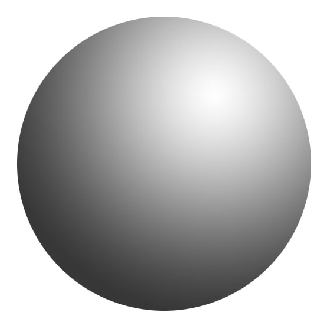
\includegraphics[height=3cm]{sphere.eps}}
	% http://www.keetee.com/downloads/sphere.jpg
	\end{pspicture}
	\end{center}
	\begin{itemize}
	 \item Gekrümmte Flächen können durch ein genügend feines \emph{Dreiecks}netz (oder Vierecksnetz) approximiert werden.
	 \item Große flache Flächen können in kleinere Dreicke zerlegt werden. 
	\end{itemize}
	\textsc{Gouraud}-Schattierung für ein Dreiecksnetz:
	\begin{itemize}
	 \item Berechne die Beleuchtung für jede Ecke eines Dreiecks , mit einem Normalvektor, der für jede Ecke fest
		ist (unabhängig von dem Dreieck zu dem es gehört). z. B. der Normalvektor der glatten Fläche, die durch
		das Dreiecksnetz approximiert wird.
		\begin{center}
		 \begin{pspicture}(0,0)(2.5,2.5)
		  \psdot(0.75,0)
		  \psdot(0,1.25)
		  \psdot(1.5,1.5)
		  \pspolygon(0.75,0)(0,1.25)(1.5,1.5)
		  \psline(2,2.25)(1.5,1.5)(2.5,1.75)
		  \psline{->}(2,0.5)(1,2.5)
		 \end{pspicture}
		\end{center}
	 \item Interpoliere die Beleuchtung linear auf jedem Dreieck
		\begin{center}
		 \begin{pspicture}(0,0)(2,2)
		  \psaxes[labels=none,ticks=none]{->}(0,0)(0,0)(2,2)
		  \psdot(0.5,0.5)\uput{3pt}[-150](0.5,0.5){5}
		  \psdot(1.5,0.5)\uput{3pt}[-30](1.5,0.5){2}
		  \psdot(1,1.5)\uput{3pt}[90](1,1.5){7}
		  \pspolygon(0.5,0.5)(1.5,0.5)(1,1.5)
		 \end{pspicture}
		\end{center}
		\[f(x,y) = ax + by + c\]
	\end{itemize}
	Die Gouraud-Schattierung, versagt z. B. bei Glanzlichtern (können verschwinden oder unnatürlich vergrößert
	werden) und sehr großen Flächen:
	\begin{center}
		\psset{Alpha=170,Beta=20}
		\begin{pspicture}(0,0)(4,3)
			\pstThreeDSquare[fillstyle=solid,fillcolor=gray](0,0,0)(4,0,0)(0,4,0)
			\pstThreeDCircle[fillstyle=solid,fillcolor=lgray,linestyle=none](2,2,0)(0.5,0,0)(0,0.5,0)
			\pstThreeDLine(4,0,0)(0,4,0)
			\pstThreeDPut(2,2,2.5){\rput{180}{
\includegraphics[width=0.6cm]{bulb.eps}}}
			\pstThreeDPut(2.5,2.5,0.1){hell?}
			\pstThreeDPut(4,0,-0.3){dunkel}
			\pstThreeDPut(0,0,-0.3){dunkel}
			\pstThreeDPut(0,4,0.3){dunkel}
			\pstThreeDPut(4,4,0.3){dunkel}
			\pstThreeDLine[linecolor=red]{->}(4,0,0)(4,2,0)
			\pstThreeDLine[linecolor=red]{->}(4,0,0)(2,0,0)
			\pstThreeDLine[linecolor=red]{->}(4,0,0)(2,2,0)
			\pstThreeDLine[linecolor=red]{->}(4,4,0)(4,2,0)
			\pstThreeDLine[linecolor=red]{->}(4,4,0)(2,4,0)
			\pstThreeDLine[linecolor=red]{->}(0,4,0)(2,2,0)
			\pstThreeDLine[linecolor=red]{->}(0,0,0)(2,0,0)
			\pstThreeDLine[linecolor=red]{->}(0,0,0)(0,2,0)
			\pstThreeDLine[linecolor=red]{->}(0,4,0)(0,2,0)
			\pstThreeDLine[linecolor=red]{->}(0,4,0)(2,4,0)
			\pstThreeDDot(0,0,0)
			\pstThreeDDot(4,0,0)
			\pstThreeDDot(0,4,0)
			\pstThreeDDot(4,4,0)
		\end{pspicture}
	\end{center}
	\textsc{Phong}-Schattierung:\\
	$\cancel{\text{diffuse Lichtquelle}}$ \emph{Umgebungslicht} (ambient light)







	\begin{itemize}
	 \item An den Ecken werden die Normalen genommen. Dazwischen werden die Normalenrichtungen angenähert
		interpoliert und mit diesen Normalen in jedem Punkt die Beleuchtungsrechnung durchgeführt
	\end{itemize}
	\begin{center}
	 \begin{pspicture}(0,0)(5,2.5)
		\psline(0,0)(1.25,1.25)(3.75,1.25)(5,0)
		\psdot(1.25,1.25)\uput{3pt}[-45](1.25,1.25){$P_1$}
		\rput(1.25,1.25){
			\psline{->}(0,0)(-0.5,0.866)\uput{3pt}[120](-0.5,0.866){$N_1$}
		}
		\psdot(3.75,1.25)\uput{3pt}[-135](3.75,1.25){$P_2$}
		\rput(3.75,1.25){
			\psline{->}(0,0)(0.5,0.866)\uput{3pt}[60](0.5,0.866){$N_2$}
		}
		\pnode(1.875,1.25){P2d}
		\rput(1.875,1.25){
			\psline[linecolor=gray]{->}(0,0)(-0.277358, 0.960767)
			\psline{->}(0,0)(-0.25,0.866)
		}
		\psline[linestyle=dashed](0.75,2.116)(4.25,2.116)
	 \end{pspicture}
	 \hspace{2cm}
	 \begin{pspicture}(0,0)(2,2.5)
		\rput(1,0.5){
			\psset{unit=1.5}
			\psdot(0,0)
			\psline{->}(0,0)(0.5,0.866)\uput{3pt}[60](0.5,0.866){$N_2$}
			\psline{->}(0,0)(-0.5,0.866)\uput{3pt}[120](-0.5,0.866){$N_1$}
			\psline[linestyle=dashed](-0.5,0.866)(0.5,0.866)
			\psline[linecolor=gray]{->}(0,0)(-0.277358, 0.960767)
			\psline{->}(0,0)(-0.25,0.866)
		}
	 \end{pspicture}
	\end{center}
	Am Punkt $\rnode{P2dformel}{P} = \lambda P_2 + (1-\lambda)P_1$ wird der folgende Normalvektor genommen:
	\nccurve[angleA=20,angleB=-90]{->}{P2dformel}{P2d}
	\[N = \frac{\lambda N_2 + (1-\lambda)N_1}{\|\lambda N_2 + (1-\lambda)N_1\|}\]
	\begin{center}
	 \psset{Alpha=190,Beta=70}
	 \begin{pspicture}(0,-0.4)(3,3.4)
	  \pstThreeDLine(2,0,0)(0,1,0)(1.5,2,0)(2,0,0)
	  \pstThreeDPut(2,0,0){
		 \pstThreeDDot(0,0,0)
		 \pstThreeDLine{->}(0,0,0)(0.416025, -0.27735, 0.866)
		 \pstThreeDPut(0.6, -0.37, 1){$N_2$}
	  }
	  \pstThreeDPut(0,1,0){
		 \pstThreeDDot(0,0,0)
		 \pstThreeDLine{->}(0,0,0)(-0.485063, -0.1213, 0.866)
		  \pstThreeDPut(-0.7, -0.2, 1){$N_1$}
	  }
	  \pstThreeDPut(1.5,2,0){
		 \pstThreeDDot(0,0,0)
		 \pstThreeDLine{->}(0,0,0)(0.223645, 0.447194, 0.866)
		 \pstThreeDPut(0.4, 0.54, 1){$N_3$}
	  }
	  \pstThreeDPut(1.16667, 1, 0){
		 \pstThreeDNode(0,0,0){P3d}
		 \pstThreeDDot(0,0,0)
		 \pstThreeDLine{->}(0,0,0)(0.0595448, 0.0188238, 0.998048)
		 \pstThreeDPut(0.16, 0.12, 1.2){$N$}
	  }
	 \end{pspicture}
	\end{center}
	\[\rnode{P3dformel}{P} = \lambda_1 P_1 + \lambda_2 P_2 + \lambda_3 P_3
		\rightarrow N = \frac{\lambda_1 N_1 + \lambda_2 N_2 + \lambda_3 N_3}
			{\|\lambda_1 N_1 + \lambda_2 N_2 + \lambda_3 N_3\|},
			\qquad (\lambda_1+\lambda_2+\lambda_3 = 1)
	\]\nccurve[angleA=20,angleB=-90]{->}{P3dformel}{P3d}
	Aufwendiger zu rechnen als Gouraud-Schattierung

	\subsection{Ausfüllen einer gerasterten Fläche}\label{sec:fill}
	\paragraph*{Annahme} Fläche ist ein Dreieck
		\[y_1 \le y_2 \le y_3\]
		$P_2$ links von $P_1P_3$
		\begin{center}
		 \vspace{5mm}
		 \begin{pspicture}(0,0)(4,5)
		  \psgrid[gridlabels=0pt,subgriddiv=2,griddots=0,gridcolor=lgray,subgridcolor=lgray,gridwidth=0.5pt,subgridwidth=0.5pt]
		  \pspolygon(0.25,3.75)(3.8,4.3)(1.73,0.2)
		  \psdot(0.25,3.75)\uput{3pt}[160](0.25,3.75){$P_2(x_2,y_2)$}
		  \psdot(3.8,4.3)\uput{3pt}[20](3.8,4.3){$P_3(x_3,y_3)$}
		  \psdot(1.73,0.2)\uput{3pt}[-90](1.73,0.2){$P_1(x_1,y_1)$}
		  \psdot[dotsize=2pt,unit=0.5](3,2)
		  \psdot[dotsize=2pt,unit=0.5](4,2)
		  \psdot[dotsize=2pt,unit=0.5](3,3)
		  \psdot[dotsize=2pt,unit=0.5](4,3)
		  \psdot[dotsize=2pt,unit=0.5](2,4)
		  \psdot[dotsize=2pt,unit=0.5](3,4)
		  \psdot[dotsize=2pt,unit=0.5](4,4)
		  \psdot[dotsize=2pt,unit=0.5](5,4)
		  \dotnode[dotsize=2pt,unit=0.5](2,5){25}
		  \dotnode[dotsize=2pt,unit=0.5](3,5){35}
		  \dotnode[dotsize=2pt,unit=0.5](4,5){45}
		  \dotnode[dotsize=2pt,unit=0.5](5,5){55}
		  \psdot[dotsize=2pt,unit=0.5](2,6)
		  \psdot[dotsize=2pt,unit=0.5](3,6)
		  \psdot[dotsize=2pt,unit=0.5](4,6)
		  \psdot[dotsize=2pt,unit=0.5](5,6)
		  \psdot[dotsize=2pt,unit=0.5](6,6)
		  \psdot[dotsize=2pt,unit=0.5](1,7)
		  \psdot[dotsize=2pt,unit=0.5](2,7)
		  \psdot[dotsize=2pt,unit=0.5](3,7)
		  \psdot[dotsize=2pt,unit=0.5](4,7)
		  \psdot[dotsize=2pt,unit=0.5](5,7)
		  \psdot[dotsize=2pt,unit=0.5](6,7)
		  \psdot[dotsize=2pt,unit=0.5](4,8)
		  \psdot[dotsize=2pt,unit=0.5](5,8)
		  \psdot[dotsize=2pt,unit=0.5](6,8)
		  \psdot[dotsize=2pt,unit=0.5](7,8)
		  \psset{unit=0.5}
		  \dotnode[dotstyle=x](1.55,5){x_l}\uput{3pt}[-160](1.55,5){$x_{\mathrm{links}}$}
		  \dotnode[dotstyle=x](5.8,5){x_r}\uput{3pt}[-20](5.8,5){$x_{\mathrm{rechts}}$}
		  \psset{angleA=40,angleB=140}
		  \nccurve{->}{x_l}{25}
		  \nccurve{->}{25}{35}
		  \nccurve{->}{35}{45}
		  \nccurve{->}{45}{55}
		  \nccurve{->}{55}{x_r}
		 \end{pspicture}
		 \vspace{5mm}
		\end{center}
		in $P_1, P_2, P_3$ sind Intensitätswerte $I_1, I_2, I_3$ berechnet worden, diese sollen linear
		interpoliert werden. (z. B. bei Gouraud-Schattierung) eigentlich sollte man die Interpolation
		in Weltkoordinten machen, und für $R, G, B$ getrennt.
		\begin{center}
		\texttt{Setpixel(\rnode{x}{$x$},\rnode{$y$}{y},$I$)}\\[1em]
		\rnode{gz}{\textrm{ganzzahlig}}
		\ncline{->}{gz}{x}
		\ncline{->}{gz}{y}
		\end{center}
		Wir füllen das Dreieck zeilenweise
		\begin{lstlisting}[mathescape=true]
FuelleZeile($x_{\mathrm{links}}$, $x_{\mathrm{rechts}}$,$y$,$I_{\mathrm{links}}$,$\Delta I$)
				// $\Delta I = I(x+1,y) - I(x,y)$ = unabhaengig von $x$ und $y$,
				// weil $I$ eine lineare Funktion ist
	$x := \lceil x_{\mathrm{links}}\rceil$
	$I := I_{\mathrm{links}} + \Delta I \cdot (x-x_{\mathrm{links}})$
	while $x \le x_{\mathrm{rechts}}$
			Setpixel($x$,$y$,$I$)
			$x := x+1$
			$I := I + \Delta I$
		\end{lstlisting}
		äußere Schleife:
		\begin{enumerate}
		 \item untere Hälfte
			\begin{align*}
			 \Delta x_{\mathrm{links}} &= \frac{x_2-x_1}{y_2-y_1} &
				\text{Ziel: auf der Geraden $P_1P_2$ gilt $x = y_1 + (y-y_1)\cdot \Delta x_{\mathrm{links}}$}\\
			 \Delta x_{\mathrm{links}} &= \frac{x_3-x_1}{y_3-y_1}\\
			 \Delta I_{\mathrm{links}} &= \frac{I_2-I_1}{y_2-y_1} &
				\text{Ziel: auf der Geraden $P_1P_2$ gilt $I = I_1 + (y-y_1)\cdot \Delta I_{\mathrm{links}}$}\\
			 \Delta I &= \frac{
					(I_1 + \Delta I_{\mathrm{rechts}})-(I_1 + \Delta I_{\mathrm{links}})
					}{
					(x_1 + \Delta x_{\mathrm{rechts}})-(x_1 + \Delta x_{\mathrm{links}})
					}\\
				  &= \boxed{\frac{\Delta I_{\mathrm{rechts}}-\Delta I_{\mathrm{links}}}
					{\Delta x_{\mathrm{rechts}}-\Delta x_{\mathrm{links}}}} &
						\text{mit $\Delta I_{\mathrm{rechts}} = \frac{I_3 - I_1}{y_3 - y_1}$}
			\end{align*}
			\begin{lstlisting}[mathescape=true]
$y = \lceil y_1 \rceil$;	$x_{\mathrm{links}}$	$:= x_1 + (y-y_1) \cdot \Delta x_{\mathrm{links}}$
	 $x_{\mathrm{rechts}}$	$:= x_1 + (y-y_1) \cdot \Delta x_{\mathrm{rechts}}$
	 $I_{\mathrm{links}}$	$:= I_1 + (y-y_1) \cdot \Delta I_{\mathrm{links}}$
while $y \le y_2$
	FuelleZeile($x_{\mathrm{links}}$, $x_{\mathrm{rechts}}$, $y$, $I_{\mathrm{links}}$, $\Delta I$)
	$y := y + 1$
	$x_{\mathrm{links}} := x_{\mathrm{links}} + \Delta x_{\mathrm{links}}$
	$x_{\mathrm{rechts}} := x_{\mathrm{rechts}} + \Delta x_{\mathrm{rechts}}$
	$I_{\mathrm{links}} := I_{\mathrm{links}} + \Delta I_{\mathrm{links}}$
			\end{lstlisting}
		 \item obere Hälfte
			\begin{lstlisting}[mathescape=true]
$\Delta x_{\mathrm{links}} := \frac{x_3 - x_2}{y_3 - y_2}$; $\Delta I_{\mathrm{links}} := \frac{I_3 - I_2}{y_3 - y_2}$
$y := y + 1$; $x_{\mathrm{rechts}} := x_{\mathrm{rechts}} + \Delta_{\mathrm{links}}$
$x_{\mathrm{links}} := x_2 + (y-y_2) \cdot \Delta x_{\mathrm{links}}$
$I_{\mathrm{links}} := I_2 + (y-y_2) \cdot \Delta I_{\mathrm{links}}$

while $y \le y_3$
	FuelleZeile($x_{\mathrm{links}}$, $x_{\mathrm{rechts}}$, $y$, $I_{\mathrm{links}}$, $\Delta I$)
	$y := y + 1$
	$x_{\mathrm{links}} := x_{\mathrm{links}} + \Delta x_{\mathrm{links}}$
	$x_{\mathrm{rechts}} := x_{\mathrm{rechts}} + \Delta x_{\mathrm{rechts}}$
	$I_{\mathrm{links}} := I_{\mathrm{links}} + \Delta I_{\mathrm{links}}$
			\end{lstlisting}
		\end{enumerate}
	\section{Entfernen verdeckter und teilweise verdeckter Flächen}
	\begin{enumerate}
	 \item Painter's Algorithmus
	 \item Tiefenpuffer
	 \item Überstreichen (swap)
	\end{enumerate}
	\begin{center}
	\begin{pspicture}(-2,-1)(2.5,2)
	 \rput{-30}{
		\psframe[fillstyle=solid](-2,0)(2,0.5)
	 }
	 \rput(2,-1){1.}
	 \rput{-5}{
		\psframe[fillstyle=solid](-1,0)(2.5,1.2)
	 }
	 \rput(3,0){2.}
	 \rput{45}(-0.5,-0.5){
		\psframe[fillstyle=solid](-1,0)(2.5,1.2)
	 }
	 \rput(1,2){3.}
	\end{pspicture}
	\end{center}

	\subsection{Painter's Algorithmus}
	Finde eine Reihenfolge der Flächen nach vorn, "`male"' die Flächen in dieser Reihenfolge.
	\paragraph*{Problem} zyklische Abhängigkeiten:
	\begin{center}
	 \begin{pspicture}(0,0)(4,3)
	 \rput{-5}(2,0.2){
		\psline[fillstyle=solid](0,0.5)(2,0.5)(2,0)(0,0)
	 }
	 \rput{-70}(2.5,1.5){
		\psframe[fillstyle=solid](-2,0)(2,1)
	 }
	 \rput{45}(1.5,1.5){
		\psframe[fillstyle=solid](-2,0)(2,0.4)
	 }
	 \rput{-5}(2,0.2){
		\psline[fillstyle=solid](0,0.5)(-2,0.5)(-2,0)(0,0)
	 }
	 \rput(5,1.5){
		\LARGE ?
	 }
	\end{pspicture}
	\end{center}
	\paragraph{Lösung} Flächen in kleinere Flächen zerlegen
	\begin{center}
	 \begin{pspicture}(0,0)(4,3)
	 \rput{-5}(2,0.2){
		\psline[fillstyle=solid](0,0.5)(2,0.5)(2,0)(0,0)
	 }
	 \rput{-70}(2.5,1.5){
		\psframe[fillstyle=solid](-2,0)(2,1)
	 }
	 \rput{45}(1.5,1.5){
		\psframe[fillstyle=solid](-2,0)(2,0.4)
	 }
	 \rput{-5}(2,0.2){
		\psline[fillstyle=solid](0,0.5)(-2,0.5)(-2,0)(0,0)
	 }
	 \rput{-5}(2,0.2){
		\psline[linestyle=dashed](0,1)(0,-0.5)
	 }
	 \rput(4.3,0.25){1.}
	 \rput(2.8,2){2.}
	 \rput(1,1.8){3.}
	 \rput(1,0){4.}
	\end{pspicture}
	\end{center}

	\subsection{Tiefenpuffer (z-Puffer)}
	Jeder Bildpunkt speichert zusätzlich einen $z$-Wert (größere Werte sind weiter hinten)
	\begin{center}
		\texttt{Setpixel($x$,$y$,$z$,$I$)} bzw. \texttt{Setpixel($x$,$y$,$z$,$I^R$,$I^G$,$I^B$)}
	\end{center}
	Vergleiche $z$ mit dem für $(x,y)$ gespeicherten $z$-Wert, wenn kleiner, dann überschreibe $z, I$, andernfalls
	ignoriere.
	
	Beim Zeichnen eines ebenen Flächenstückes ist $z$ linear von $x$ und $y$ abhängig. $z$ interpoliert zwischen
	den 3 Ecken $P_i(x_i,y_i,z_i), i = 1, 2, 3$
	\paragraph{Nachteil} (von beiden Verfahren) Aufwand ist proportional zu gezeichneten Gesamtfläche und nicht
 	zur sichtbaren Fläche (nicht sichtbare Flächen werden auch gezeichnet bzw. zu zeichnen versucht).




\section{Darstellung einer Szene durch Überstreichen (Scanline-Algorithmus)}
\paragraph*{Vereinfachte Annahme} Szene besteht auzs Dreiecken.
\begin{itemize}
 \item Der Algorithums beruht auf der gleichen Idee wie der Algorithmus zum Ausfüllen gerasterter Flächen
	(s. Abschnitt \ref{sec:fill})
	\begin{itemize}
	 \item Überstreiche Szenee mit horizontalen Geraden (von unten nach oben, mit steigendem $y$)
		\begin{itemize}
		 \item Für jede Rasterzeile gehe Pixel von links nach rechts durch (mit steigendem $x$)
		\end{itemize}
	\end{itemize}
 \item Prinzip: Der Algorithmus aus Abschnitt \ref{sec:fill} wird für alle Dreiecke parallel angewendet
\end{itemize}
\begin{center}
 \begin{pspicture}(0,0)(5,4)
  \psframe(0,0)(5,4)
  \rput[l](0,0.2){\psline(0,0)(5,0)}
  \rput[l](0,0.4){\psline(0,0)(5,0)}
  \rput[l](0,0.6){\psline(0,0)(5,0)}
  \rput[l](0,0.8){\psline(0,0)(5,0)}
  \rput[l](0,2.7){\psline(0,0)(5,0)}
  \pspolygon(3.5,0.6)(4,3)(1,1)
  \pspolygon(0.5,1.4)(1,3.2)(4.5,0.9)
 \end{pspicture}
\end{center}
\begin{description}
\item[Vorverarbeitung] Wir erstellen eine Kantenliste (Edge List, EL), sortiert nach den Koordinaten des unteren Endpunktes der Kante,
	zuerst nach der $y$-Koordinate sortiert, bei gleicher $y$-Koordinate nach $x$-Koordinate
	(horizontal Kanten brauchen nicht gespeichert werden).
\item[Bearbeitung einer Zeile] Wir benötigen zur Abarbeitung einer Zeile die Menge der von der Zeile
	geschnittenen Dreiecke und für diese dann die nötigen Parameter, wie sie für die Fülle-Zeile-Funktion aus
	Abschnitt \ref{sec:fill} benutzt wurden.

	Wir verwalten die Daten in einer \emph{"`Aktive-Kanten-Liste"'} (AEL). Darin enthalten sind alle Kanten, die
	die aktuelle Scanline schneiden. Sie sind sortiert nach der $x$-Koordinate des Schnittpunktes mit der Scanline.
	Zu jeder Kante speichern wir die Informationen, die wir benötigen. Um das Dreieck für diese Zeile zu rastern und
	die entsprechenden Werte für die Zeile auszurechnen.

	z. B.
	\begin{itemize}
	\item zugehöriges Dreieck
	\item linke oder rechte Begrenzung
	\item $y$-Koordinate des oberen Endpunktes (um die Kante au der AEL entfernen zu können)
	\item $x$-Koordinate Schnittpunktes mit der Scanline (entspricht $x_{\mathrm{links}}$ bzw. $x_{\mathrm{rechts}}$)
	\item $\Delta x$ (entspricht $\Delta x_{\mathrm{links}}$ bzw. $\Delta x_{\mathrm{rechts}}$)
	\end{itemize}
	die folgenden Daten brauchen nur in einer linken Begrenzung gespeichert werden:
	\begin{itemize}
	 \item $z_{\mathrm{links}}, I_{\mathrm{links}}, \Delta z_{\mathrm{links}}, \Delta I_{\mathrm{links}}, \Delta z,
		\Delta I$ (Notation s. Abschnitt \ref{sec:fill})
	\end{itemize}
	und entsprechende Werte für andere zu interpolierende Daten.
\item[Änderung der AEL beim Übergang von $\boldsymbol{y}$ auf $\boldsymbol{y+1}$] wie bei der äußeren Schleife in
	Abschnitt \ref{sec:fill}.
	\begin{itemize}
	 \item inkrementiere $x, z_{\mathrm{links}}, I_{\mathrm{links}}$ um $\Delta x, \Delta z_{\mathrm{links}},
		\Delta I_{\mathrm{links}}$
	\end{itemize}
	Außerdem kann es nötig sein Kanten aus der Liste zu löschen (Kante endet zwischen $y$ und $y+1$),
	neue Kanten aufzunehmen (Kante beginnt zwischen $y$ und $y+1$) oder die Reihenfolge der Kanten zu ändern
	(Kanten schneiden sich zwischen $y$ und $y+1$)
	\begin{enumerate}
	 \newcommand{\bs}{\boldsymbol}
	 \item \textbf{Kante endet zwischen $\bs y$ und $\bs{y+1}$}\\
		Vergleiche $y$-Koordinate des oberen Endpunktes einer Kante in der AEL mit der aktuellen
		Scanline-Koordinate
	 \item \textbf{Kante beginnt zwischen $\bs y$ und $\bs{y+1}$}\\
		Vergleiche $y$-Koordinate des unteren Endpunktes der ersten noch nicht verwendeten Kante in der EL
		mit aktuellen Scanline-Koordinaten.
	 \item \textbf{Kanten schneiden sich zwischen $\bs y$ und $\bs{y+1}$}\\
		prinzipiell vergleiche die neuen $x$-Werte zweier Kanten die in der alten AEL benachbart waren
		\paragraph*{Problem} Die Scanline wird nicht Kontinierlich
		\begin{center}
		 \begin{pspicture}(0,0)(5,1)
		  \psline(0,0)(5,0)\uput{3pt}[180](0,0){$y$}
		  \psline(0,1)(5,1)\uput{3pt}[180](0,1){$y+1$}
		  \psline(1,1)(4,0)
		  \psline(1.2,0)(2.5,1)
		  \psline(1.4,0)(1.2,1)
		  \psline(1.5,0)(1.8,1)
		  \psline(2.3,0)(2,1)
		  \psline(2.7,0)(2.3,1)
		  \psline(2.9,0)(2.87,1)
		  \psline(3.1,0)(3.13,1)
		  \psline(3.2,1)(4.2,0)
		  \psline(1.4,0)(2.7,1)
		  \psline(1.6,0)(2.9,1)
		  \psline(1.9,0)(2.9,1)
		  \psline(2.1,0)(3.4,1)
		 \end{pspicture}
		\end{center}
		Es können sich auch nichtbenachbarte Kanzen zwischen $y$ und $y+1$ schneiden, wenn die dazwischen
		liegenden Kanten ebenfalls geschnitten werden. Wir müssen also nicht nur bei $y$ benachbarte Kanten
		vergleichen, sondern auch die nache einer Kreuzung entstehenden neuen Nachbarn.

		Dieser Ansatz läuft auf ein Buble-Sort- oder Insertion-Sort-Prinzip hinaus. Dann ist Neusortieren
		mit effizienten Sortierverfahren.
	\end{enumerate}
\item[Füllen einer Zeile] Zeile wird von links nach rechts durchlaufen. Beachten wir dabei die Tiefeninformation
	entspricht dies einem Überstreichen einer Ebene $y = \mathbf{const}$ mit einer Geraden $x = \mathbf{const}$
	\begin{center}
	 \psset{unit=1.5}
	 \begin{pspicture}(0,-0.2)(4,2.2)
	  \psaxes[ticks=none]{->}(0,0)(0,0)(4,2)
	  \uput{3pt}[135](0,2){$z$}
	  \uput{3pt}[-45](4,0){$x$}
	  \psline{*-*}(1,1.75)(3,0.5)
	  \uput{3pt}[90](1,1.75){Kante $AB$}
	  \uput{3pt}[-45](3,0.5){Kante $AC$}
	  \rput[tr](2,1.125){
		\begin{minipage}{2.7cm}
			Schnitt mit dem Dreieck $ABC$
		\end{minipage}
	   }
	  \psline{*-*}(2.5,1.125)(3.5,2)
	  \uput{3pt}[-45](2.5,1.125){Kante $DE$}
	  \uput{3pt}[90](3.5,2){Kante $DF$}
	  \rput[tl](3,1.5025){Schnitt mit dem Dreieck $DEF$}
	 \end{pspicture}
	\end{center}
	in dieser Ebene haben wir Kante, die den Schnitten von Dreiecken mit der Ebene entsprechen. Der Dreiecksschnitt,
	dessen $z$-Koordinate für ein gegebenes $x$ am kleinsten ist, bestimmt die Färbung des Pixels.

	Analog zur AEL legen wir eine aktive Dreiecksliste (ATL, auch active span list) an, om der die von der aktiven
	Geraden $x = \mathbf{const}$ geschnittenen Dreiecksschnitte nach $z$-Koordinate sortiert sind und die zugehörigen
	Werte für die Interpolation gespeichert sind. Das sind $z, I$ und $\Delta z$, sowie $\Delta I$ und $x_{\mathrm{rechts}}$.

	Modifizierung der ATL beim Übergang von $x$ auf $x+1$
	\begin{enumerate}
	 \item Dreieck einfügen: $x_{\mathrm{links}}$ liegt zwischen $x$ und $x+1$ für eine linke
		Kante in der AEL
	 \item Dreieck löschen: $x_{\mathrm{rechts}}$ liegt zwischen $x$ und $x+1$
	 \item Zwei Dreiecke schneiden sich ($z$-Werte tauschen Reihenfolge)
	\end{enumerate}
	zu zeichnen ist die aktuelle Farbe des Dreiecks, das in der ATL aktuell an der ersten Stelle steht.
\end{description}
\subsubsection{Varianten, Sonderfälle, ...}
\begin{enumerate}
 \item Es ist häufig sinnvoll, sobald zwei Kanten in der AEL benachbart werden, den Schnittpunkt zu berecnhen und
	diesen, falls er existiert, in einem \emph{Event-Schedule} einzufügen. Dieser verwaltet die "`Zeit"'-punkte,
	an denen sich die Reihenfolge der Kanten ändert in einer Prioritätswarteschlange.
 \item Vereinfachungen bei sich nicht schneidenden Dreiecken
 \item Kombination mit dem Tiefenpuffer\\
	z. B. tiefenpuffer für eine Zeile des Bildes
	\begin{itemize}
	 \item Überstreiche Szene zeilenweise
	 \item Vor jedem Wechsel in eine neue Zeile leere Tiefenpuffer
	 \item für jede Zeile: Zeichne alle Dreiecke in der aktuellen AEL (in beliebiger Reihenfolge) nach dem
		Tiefenpuffer-Prinzip
	\end{itemize}
	Analog: Tiefenpuffer für ein Pixel
	\begin{center}
	 \begin{tabular}{p{.45\linewidth}|p{.45\linewidth}}
	  Größe des Tiefenpuffers & Struktur des Algorithmus\\
	  \hline\hline
		Breite $\times$ Höhe $\times$ Genauigkeit &
		\begin{minipage}{\linewidth}
		 \vspace{1em}
		 \begin{verbatim}
Für alle Dreiecke
    Für alle Zeilen
        Für alle Spalten
		 \end{verbatim}
		\end{minipage}\\
		\hline
		Breite $\times$ Genauigkeit &
		\begin{minipage}{\linewidth}
		 \vspace{1em}
		 \begin{verbatim}
Für alle Zeilen
    Für alle Dreiecke
        Für alle Spalten
		 \end{verbatim}
		\end{minipage}\\
		\hline
		Genauigkeit &
		\begin{minipage}{\linewidth}
		 \vspace{1em}
		 \begin{verbatim}
Für alle Zeilen
    Für alle Spalten
        Für alle Dreiecke
		 \end{verbatim}
		\end{minipage}\\
	 \end{tabular}
	\end{center}
\end{enumerate}





\section{Anzeigen von benachbarten Flächenstücken (Dreiecken)}
\begin{center}
 \psset{unit=0.5,gridcolor=gray,gridlabels=0pt}
 \begin{pspicture}(0,0)(7,9)
  \psgrid
  \pspolygon(6.6,8.7)(0.3,3.4)(5.8,5.4)
  \pspolygon(2.3,-0.1)(0.3,3.4)(5.8,5.4)
  \pspolygon(2.3,-0.1)(5.8,5.4)(7,2.3)
  \psline[linewidth=0.5pt]{->}(5,4)(5.5,4)
  \psdot(3,4)\psdot(4,4)\psdot[dotstyle=o](5,4)\uput{3pt}[-45](5,4){?}
  \psdot(2,3)\psdot(3,3)\psdot(4,3)
  \psline[linewidth=0.5pt]{->}(6,5)(7,5)
  \psdot(6,5)
 \end{pspicture}
\end{center}
Gehört der Rand eines Dreiecks zum Dreieck?\\
Zu welchem Dreieck?
\paragraph*{Gesucht} Eine konsistente Regel, die bei mehreren aneienanderstoßenden Flächen feslegt, zu welcher Fläche
jeder Bildpunkt gehört.
\paragraph*{Eine Möglichkeit} Ein Pixel, das auf dem Rand liegt wird (in Gedanken) horizontal nach rechts verschoben.
	Es gehört zu der Fläche, wo es dann landet. Wenn es dabei auf einer horizontalen Kante liegt, dann wird es zur
	oberen Fläche gerechnet.
\begin{center}
 \psset{unit=0.5}
 \begin{pspicture}(0,0)(11,7)
  \psline[linewidth=1.7pt](1,7)(0,5)(1,3)(4,3)
  \psline(4,3)(5,5)
  \psline[linewidth=1.7pt](5,5)(7,3)(4,0)(9,0)
  \psline(9,0)(9,4)(9,4)(11,7)(1,7)
  \psline[linewidth=0.5pt]{->}(0.5,4)(1.5,4)
  \psline[linewidth=0.5pt]{->}(4.5,4)(5.2,4)
  \psline[linewidth=0.5pt]{->}(9,2)(10,2)
  \psline[linewidth=0.5pt]{->}(10,5.5)(11,5.5)
 \end{pspicture}
\end{center}
\paragraph*{Vorraussetzung} Exakte Arithmetik

\section{Lineare Interpolation in Weltkoordinaten}
Interpolation von Helligkeitswerden (Gouraud-Schattierung), von Normalenrichtungen (Phong-Schattierung), bei Texturen
immer in \emph{Weltkoordinaten}! Nicht NDC.
\paragraph{Gegeben} Eine Strecke $P_1P_2$ in NDC (oder Bildschirmkoordinaten) als Bild einer Strecke $P_1P_2$
	in Weltkoordinaten.

	An den Endpunkten sind Werte $I_1, I_2$ gegeben

	(Intensitätswerte $I_1^R, I_1^G, I_1^B,...$, oder
	Normalenrichtungen $N_1^x, N_1^y, N_1^z,...$)

	Wir wollen diese Werte für die dazwischen liegenden Punkte der Strecke in Weltkoordinaten interpolieren.

	\hrulefill

	Wir kennen die Transformationsmatrix $M = M^{\mathrm{Welt, NDC}}$:
	\[ M \vfour{x_{\mathrm{Welt}}}{y_{\mathrm{Welt}}}{z_{\mathrm{Welt}}}{w_{\mathrm{Welt}}}
		= \vfour{x_{\mathrm{NDC}}}{y_{\mathrm{NDC}}}{z_{\mathrm{NDC}}}{w_{\mathrm{NDC}}}
	\qquad\qquad P_1 = \vfour{x_1^{\mathrm{NDC}}}{y_1^{\mathrm{NDC}}}{z_1^{\mathrm{NDC}}}{1}
	\qquad P_2 = \vfour{x_2^{\mathrm{NDC}}}{y_2^{\mathrm{NDC}}}{z_2^{\mathrm{NDC}}}{1}\]
	\[P_1\text{ in homogenen Weltkoordinaten} = M^{-1} \vfour{x_1^{\mathrm{NDC}}}{y_1^{\mathrm{NDC}}}{z_1^{\mathrm{NDC}}}{1}
	 = \vfour{x_1^{\mathrm{Welt}}}{y_1^{\mathrm{Welt}}}{z_1^{\mathrm{Welt}}}{w_1^{\mathrm{Welt}}}
	 \hat = \vthree{x_1^{\mathrm{Welt}}/w_1^{\mathrm{Welt}}}{y_1^{\mathrm{Welt}}/w_1^{\mathrm{Welt}}}
		{z_1^{\mathrm{Welt}}/w_1^{\mathrm{Welt}}}\text{ in kartesischen Weltkoordinaten}
	\]
\paragraph{Annahme:} $I: \mathbb{R}^3 \to \mathbb{R}$ linear $I(P_1) = I_1 \qquad I(P_2) = I_2$

\hrulefill

Betrachte eine "`homogene Erweiterung"': $\hat I: \mathbb{R}^4 \to \mathbb{R}$ von I
\[\hat I\left(\vfour{\lambda x}{\lambda y}{\lambda z}{\lambda w}\right) =
	\lambda \cdot \hat I\left(\vfour{x}{y}{z}{w}\right)
	\qquad
	\hat I\left(\vfour{x}{y}{z}{1}\right) = I\left(\vthree{x}{y}{z}\right)\]
\begin{enumerate}
 \item Die Funktion $\hat I$ ist linear;
 \item Aus $\hat I$ kann man $I$ ausrechnen:
	\[I\left(\text{Punkt $\vfour{x}{y}{z}{w}$ in homogenen Koordinaten}\right) = \frac{1}{w} \cdot
		\hat I\left(\vfour{x}{y}{z}{w}\right)\]
\end{enumerate}
\begin{align*}
 I\left(\text{Punkt in homogenen Koordinaten }\vfour{x}{y}{z}{w}\right) &= \\
 I\left(\text{Punkt in homogenen Koordinaten }\vfour{x/w}{y/w}{z/w}{1}\right) &=
	\hat I \left(\vfour{x/w}{y/w}{z/w}{1}\right) = \frac{1}{w} \cdot \hat I\left(\vfour{x}{y}{z}{w}\right)\\
 I\left(\text{Punkt in karthesischen Koordinaten }\vthree{x/w}{y/w}{z/w}\right) &=
\end{align*}

\begin{enumerate}
 \item Berechne $P_1$ und $P_2$ in homogenen Weltkoordinaten:
	\[\vfour{x_1^{\mathrm{Welt}}}{y_1^{\mathrm{Welt}}}{z_1^{\mathrm{Welt}}}{w_1^{\mathrm{Welt}}}
	= M^{-1} \cdot \vfour{x_1^{\mathrm{NDC}}}{y_1^{\mathrm{NDC}}}{z_1^{\mathrm{NDC}}}{1}
	\text{ und } \vfour{x_2^{\mathrm{Welt}}}{y_2^{\mathrm{Welt}}}{z_2^{\mathrm{Welt}}}{w_2^{\mathrm{Welt}}}
	= M^{-1} \cdot \vfour{x_2^{\mathrm{NDC}}}{y_2^{\mathrm{NDC}}}{z_2^{\mathrm{NDC}}}{1}\]
 \item Berechne $\hat I_1$ und $\hat I_2$ an diesem Punkt in $\mathbb{R}^4$
	\begin{align*}
	 I(P_1) =\ &I_1 = \frac{1}{w} \cdot \hat I_1\\
		&\boxed{\hat I_1 = w_1^{\mathrm{Welt}} \cdot I_1,\ \hat I_2 = w_2^{\mathrm{Welt}} \cdot I_2}
	\end{align*}
 \item Lineare Interpolation $P(\lambda) = \lambda_2 + (1 - \lambda) P_1$ in NDC
	\paragraph{Gesucht} $I(\lambda) = I(P(\lambda))$
		\[\vfour{x(\lambda)}{y(\lambda)}{z(\lambda)}{1} = \lambda \vfour{x_2}{y_2}{z_2}{1}
			+ (1-\lambda) \vfour{x_1}{y_1}{z_1}{1} \]
		\[\boxed{\hat I = \lambda \cdot \hat I_2 + (1-\lambda) \hat I_1}\]
		\[\boxed{w^{\mathrm{Welt}}(\lambda) = \lambda \cdot w^{\mathrm{Welt}}_2 + (1-\lambda) w^{\mathrm{Welt}}_1}
		\qquad I(\lambda) = \frac{\hat I(\lambda)}{w^{\mathrm{Welt}}(\lambda)}\]
\end{enumerate}
\paragraph*{Zusammenfassung} $w_1^{\mathrm{Welt}}, w_2^{\mathrm{Welt}} = $ letzte Komponente von $M^{-1} \vthree{\ }{\cdots}{\ }$
	\[\boxed{I(\lambda)} = \frac{\overbrace{w_2^{\mathrm{Welt}} \cdot I_2}^{\hat I_2} \cdot \lambda
		+ \overbrace{w_1^{\mathrm{Welt}} \cdot I_1}^{\hat I_1} \cdot (1-\lambda)}
					{w_2^{\mathrm{Welt}} \lambda + w_1^{\mathrm{Welt}} (1 - \lambda )}\]

\paragraph{Einbau in Füllalgorithmus}
 \rnode{zus}{zusätzlich}

\begin{lstlisting}[mathescape=true,backgroundcolor=\color{white}]
FuelleGerade($x_1$, $x_2$,$y$,$z_1$,$z_2$,$\rnode{w1}{w_1}$,$\rnode{w2}{w_2}$,$I_1$,$I_2$)
	$\hat I_1 = w_1 I_1$
	$\hat I_2 = w_2 I_2$
	$\Delta \hat I = ...$
	$\Delta w = ...$
	$\vdots$
	while $x < x_2$
			Setpixel($x$,$y$,...,$I$)
			$x := x+1$
			$z := z + \Delta z$
			$\hat I := \hat I + \Delta I$	// Zaehler
			$w := w + \Delta w$		// Nenner
			$I = \tfrac{\hat I}{w}$
\end{lstlisting}
\ncline{->}{zus}{w1}
\ncline{->}{zus}{w2}
analog für mehrere Größen $I^R, I^G, I^B$ nimmt man $\hat I^R$, $\hat I^G$, $\hat I^B$, 
$w$ und $\Delta w$ braucht man nur einmal.

\paragraph{Bemerkung} Die $z$-Koordinate kann man direkt in NDC interpolieren

\section{Transformation von Normalvektoren bei affinen Transformationen}
z. B. Objektkoordinaten auf Weltkoordinaten
\begin{center}
 \psset{Alpha=170,Beta=20}
 \begin{pspicture}(-1,-3)(7,5)
  \rput[tl](0,3.5){
		\pspolygon(-1,0)(1,0)(0,1)
		\psline{*->}(0.5,0.5)(1.207,1.207)
		\psline[linewidth=0.3pt](0,0)(0,1)
  }
  \rput[tl](0,0){
	\psline[linestyle=dashed](-1.5,3)(1.5,3)
	\pstThreeDLine(-1,-1,0)(1,-1,0)(1,1,0)(-1,1,0)(-1,-1,0)
	\pstThreeDLine(-1,-1,0)(0,0,1)(1,1,0)
	\pstThreeDLine[linewidth=0.3pt](0,0,0)(0,0,1)
	\pstThreeDLine(-1,1,0)(0,0,1)(1,-1,0)
	\pstThreeDLine{*->}(0.5,0,0.5)(1.207,0,1.207)
	\pstThreeDPut(2.9,0,1.907){
		\begin{minipage}{6cm}
		\centering
		$\left(\pm\dfrac{1}{\sqrt{2}},0,\dfrac{1}{\sqrt{2}}\right)$ bzw.
		$\left(0, \pm\dfrac{1}{\sqrt{2}},\dfrac{1}{\sqrt{2}}\right)$ \\
		(Normalenrichtungen)
		\end{minipage}}
	\pstThreeDPut(0,0,1.2){$(0,0,1)$}
	\pstThreeDPut(2,1,0){$(\pm 1,\pm 1,0)$}
  }
  \rput[tl](3.5,0.2){
	\pspolygon(0,0)(1,0)(1,-0.2)(1.5,0.3)(1,0.8)(1,0.6)(0,0.6)
  }
  \rput[tl](7.5,-2){
	\pstThreeDBox(-0.5,0.5,0)(1,0,0)(0,-1,0)(0,0,2)
	\pstThreeDLine(-0.5,-0.5,2)(0,0,4)(0.5,0.5,2)
	\pstThreeDLine[linestyle=dashed](-0.5,0.5,2)(0,0,4)
	\pstThreeDLine(0.5,-0.5,2)(0,0,4)
	\pstThreeDPut(0,-1,2){$b$}
	\pstThreeDPut(0,0,2.3){$G$}
	\pstThreeDDot(0,0,2)
	\pstThreeDLine{<->}(-0.65,-0.15,2)(-0.65,-0.15,4)
	\pstThreeDPut(-0.8,-0.5,3){$h$}
  }
 \end{pspicture}
\end{center}
\[T = \begin{pmatrix}
       \nicefrac{b}{2} & 0 & 0 & g_x\\
       0 & \nicefrac{b}{2} & 0 & g_y\\
       0 & 0 & h & g_z\\
       0 & 0 & 0 & 1
      \end{pmatrix}
\]
\[T = \begin{pmatrix}
       A & \vline & b\\
       \hline
       0 & \vline & 1
      \end{pmatrix} \qquad
      \vthree{x}{y}{z} \mapsto \underbrace{A \vthree{x}{y}{z} + b}
\]
\paragraph*{Ebene im Urbildraum}
\begin{align*}
 E &= \left\{\left.\vec x = \vthree{x}{y}{z}\ \right|\ \vec n^T \cdot \vec x = c\right\}
 \qquad \vec n... \text{Normalenvektor, } c \in \mathbb{R}\\
 T(E) &= \{\underbrace{A \cdot \vec x + b}_{= \bar x}\ |\ \vec n^T \cdot \vec x = c\}
\end{align*}
\[Ax + b = \bar x \qquad x = A^{-1}(\bar x - b)\]
\begin{align*}
 T(E) 	&= \left\{\bar x\ \left|\ n^T A^{-1} \left(\bar x - b\right) = c\right.\right\}\\
	&= \left\{\bar x\ \left|\ n^T A^{-1} \bar x = c + n^T A^{-1} b\right.\right\}\\
	&= \Big\{\bar x\ \Big|\ \underbrace{\left(\left(A^{-1}\right)^Tn\right)^T}_{\text{Normalvektor der Ebene} T(E)} \bar x = \bar c\Big\}
\end{align*}

Bei einer Affinen Transformation mit $3 \times 3$-Transformationsmatrix $A$ muss man Nornalvektoren nicht
mit $A$, sondern von links nach rechts mit $(A^{-1})^T$ multiplizieren und anschließend \emph{normieren}.
(Vektoren als Spalten betrachten)

Falls $A$ orthogonal ist, dann ist $A^T = A^{-1}$, $(A^{-1})^T = A$
\begin{center}
 \begin{pspicture}(-2,-0.4)(1,2)
	\pspolygon(-1,0)(1,0)(0,1)
	\psline{*->}(0.5,0.5)(1.207,1.207)
	\psline[linewidth=0.3pt](0,-0.4)(0,1.4)
	\uput{3pt}[45](1.207,1.207){$\vec n$}
	\psline[linewidth=0.3pt](-2,0)(-0.5,1.5)
	\psline[linewidth=0.3pt](-1.8,0)(-0.3,1.5)
	\psline[linewidth=0.3pt](-1.6,0)(-0.1,1.5)
	\psline{->}(0,1)(1,2)
 \end{pspicture}
 \hspace{2cm}
 \begin{pspicture}(-2,-0.4)(1,2)
	\pspolygon(-0.25,0)(0.25,0)(0,1)
	\psline{->}(0.125,0.5)(0.302,1.207)
	\uput{3pt}[75.96](0.302,1.207){$A \cdot \vec n$}
	\psline[linewidth=0.3pt](-0.5,0)(-0.125,1.5)
	\psline[linewidth=0.3pt](-0.45,0)(-0.075,1.5)
	\psline[linewidth=0.3pt](-0.4,0)(-0.025,1.5)
 \end{pspicture}
\end{center}





\chapter{Texturen}
\emph{(Abbildungen folgen später)}\\
Aufbringen eines Musters auf eine Fläche.\\[1em]
% 15.1
Das Muster -- die Textur -- ist als zweidimensionales \emph{Bild} gegeben (Pixelarray), und eine Abbildung
von diesem Bild auf eine Fläche im Raum.\\[1em]
% 15.2
Die Bildfläche muss nicht unbedingt flach sein:
\begin{enumerate}
 \item gekrümmt % 15.3
 \item Dreiecksgitter % 15.4
	Dann muss man das Bild in ein Dreicksgitter mit derselben kombinatorischen Struktur zerlegen.
	Die Abbildung erfolgt dann durch lineare Interpolation auf jedem Dreieck.
\end{enumerate}
Bei beiden Lösungen existiert das Problem der Verzerrung.\\[1em]
Einfaches Modell für Architektur: Fassade wird auf die Hasuwand aufgeklebt.
% 15.5
\paragraph*{Problem} Schatten sind möglicherweise nicht richtig.

Bei der Darstellung benötigt man die Umkehrabbildung von der Fläche in Weltkoordinaten
(bzw. von der projezierten Fläche in NDC) auf die Textur.

Bei der linearen Interpolation von \emph{Dreiecken} verwendet man gerne \emph{baryzenztische Koordinaten}
\begin{center}
 % 15.6
\end{center}
\[(\lambda_1, \lambda_2, \lambda_3) \text{ mit } \lambda_1 + \lambda_2 + \lambda_3 = 1\]
stellt den Punkt $\lambda_1 A_1 + \lambda_2 A_2 + \lambda_3 A_3$ dar.
\[\lambda_1, \lambda_2, \lambda_3 \ge 0 \Leftrightarrow \text{ Punkt im Dreieck}\]
\begin{center}
 % 15.7
\end{center}
Die Ecken des Dreiecks auf dem Objekt haben barizentrische Koordinaten
\[(\lambda_1, \lambda_2, \lambda_3) = (1,0,0), (0,1,0), (0,0,1)\]
dazwischen wird linear \emph{interpoliert} (in Weltkoordinaten). Dann nimmt man in der Textur den Punkt an der
Stelle $\lambda_1 B_1 + \lambda_2 B_2 + \lambda_3 B_3$.
\begin{center}
 % 15.8+9
\end{center}
Möglcihe Probleme dadurch, das Auflösung des erzeugten bilder nicht mit der Auflösung der Textur übereinstimmt.
\begin{enumerate}[a)]
 \item Auflösung der Textur zu klein\\
	$\Rightarrow$ Bild wirkt grob gepixelt (mögliche Lösung: Interpolation)
 \item Auflösung der Textur ist größer\\
	$\Rightarrow$ Es kann zu Aliasing-Effekten kommen. (mögliche Auswege s. Abschnitt \ref{sec:antialiasing})
\end{enumerate}

\chapter{Schatten}
\begin{center}
 %13.10
\end{center}
Für die Berecnhung von chatten kann man die gleichen Methoden verwenden, wie zur Bestimmung sichtbarer Flächen:
\begin{itemize}
 \item von der Lichtquelle aus "`sichtbar"' $\Rightarrow$ beleuchtet.
 \item von der Lichtquelle aus "`verdeckt"' $\Rightarrow$ Schatten.
\end{itemize}
\begin{enumerate}
 \item Berechne (für jede Lichtquelle unabhängig) in einem getrennten Puffer das "`Bild"', dass von der Lichtquelle aus
	"`gesehen"' wird.\\
	z. B. mit dem Tiefenpuffer \lstinline[mathescape=true]!PutPixel($x$,$y$,$z$,$\rnode{I}{I}$)!
	\begin{center}
	 \rnode{Index}{Index} (Nummer) der Fläche, die gerade dargestellt wird.
	 \ncangle[angleA=90,angleB=-90]{->}{Index}{I}\\
	 % 13.11
	\end{center}
 \item Erzeuge das Bild, dass vom Auge aus sichtbar ist Pixel für Pixel.
	\begin{center}
	 % 13.12
	\end{center}
	$P$ sei der Punkt (in Weltkoordinaten), der gerade dargestellt wird. Er gehört zum Objekt mit Nummer $n$.
	Bestimme das Bild von $P$ im Bildpuffer, der zur Lichtquelle gehört und vergleiche den Index, der dort
	gespeichert ist.

	Wenn $= n \Rightarrow $ Punkt $P$ ist von dieser Lichtquelle beleuchtet.
\end{enumerate}
\chapter{Clipping}
Eine Strecke auf ein Rechteck zurechtstutzen.
\begin{center}
 % 15.13
\end{center}
\section{Algorithmus von Cohen-Sutherland}
$\mathbb{R}^2 \to \{0,1\}^4 \qquad$ (4 Bits)
\begin{align*}
 x &< x_\mathrm{min} \\
 x &> x_\mathrm{max} \\
 y &< y_\mathrm{min} \\
 y &< y_\mathrm{max} \\
\end{align*}
\begin{enumerate}
 \item Wenn $A_1$ und $A_2$ ein gemeinsames 1-Bit haben.\\
	$\Rightarrow$ Strecke $A_1A_2$ schneidet Rechteck nicht.
 \item Wenn beide Codes 0000 sind.\\
	$\Rightarrow$ Strecke liegt zur Gänze im Inneren.
 \item Bestimme eine Stelle, wo sich beide Codes unterscheiden,
 \item Schneide die Gerade mit der entsprechenden horizontalen oder vertikalen Geraden.
 \item Ersetze den Endpunkt mit dem 1-Bit durch den Schnittpunkt.
 \item Wiederhole
\end{enumerate}





\end{document}
